\documentclass[twoside,english,headsepline=on,DIV=12]{scrartcl}

\usepackage{shellesc}
\usepackage{amsmath}
\usepackage{fontspec}
\usepackage{unicode-math}
\setmainfont{TeX Gyre Pagella}
%\setsansfont{DejaVu Sans}
%\setmonofont{Inconsolata}
\setmathfont{TeX Gyre Pagella Math}
%\addtokomafont{disposition}{\normalfont\sffamily}
%\usepackage[utf8]{inputenc}
%\usepackage[T1]{fontenc}
%\usepackage{stix}
%\usepackage{color}
%\usepackage{enumitem}
\usepackage[english]{babel}
\usepackage{icomma}
\usepackage{graphicx}
\numberwithin{equation}{section}
\usepackage{siunitx}
\usepackage{physics}

%%\usepackage{titlesec}
\usepackage{tikz}
\usetikzlibrary{external}
\tikzexternalize
\tikzsetexternalprefix{figures/}
\usepackage{gnuplot-lua-tikz}
%\usetkzobj{all}
%\usepackage{adjustbox}
\usepackage{multirow}
\usepackage{url}
%\urlstyle{same}
\usepackage{wrapfig}
\usepackage[font=small, labelfont=bf]{caption}
\usepackage{subcaption}
\usepackage{booktabs} 
%\usepackage[]{geometry}
\usepackage[section]{placeins}
\usepackage{pdflscape}
%\usepackage{showframe}
%\usepackage{MnSymbol}
%\usepackage[disable]{todonotes}
\usepackage{extarrows}
\usepackage[
	backend=biber 
]{biblatex}
\addbibresource{plasmons.bib}
\usepackage{csquotes} 
\usepackage{import}
%\usepackage{fancyhdr}
\pagestyle{headings}

\begin{document}
\titlehead{{\Large Universität Stuttgart
\hfill SS 19\\}
Physikalisches Praktikum II}
\subject{Laboratory Report}
\title{Surface Plasmons}
\author{David Hoffmann, Marius Tochtermann \\
Group B30}
\publishers{}
\date{15.04.2019}
\maketitle
\begin{abstract}
\end{abstract}
\tableofcontents
\newpage
\section{Theory}
In order to describe surface plasmons the Maxwell equations are needed, as they are the theoretical fundament of electrodynamics. The four Maxwell equations lead to four boundary conditions at the transition area between two optical mediums, from which two apply to the electric field and two apply to the magnetic field. 

The first maxwell equation
\begin{align}
\vec{\nabla} \cdot \vec{D} = \vec{\nabla} \cdot \vec{E}\cdot \epsilon_0 \cdot \epsilon_\text{r} =  \rho_\text{frei} \label{eq:Maxwell1}
\end{align}
leads to the condition that the electric flux density needs to be steady in the direction perpendicular to the transition surface, as the density of electrical charges $\rho_\text{frei}$ equals zero inside the transition area. Due to the fact that the $\epsilon_\text{r}$ of the two media are not the same, the electric field is not steady.

Like the first Maxwell equation describes the electric flux density, the second Maxwell equation is about the magnetic flux density. Thus that no magnetic monopoles exist, the right side of the second Maxwell equation
\begin{align}
\vec{\nabla} \cdot \vec{B} = \vec{\nabla} \cdot \vec{H}\cdot \mu_0 \cdot \mu_\text{r} =  0 \label{eq:Maxwell2}
\end{align}
always equals zero. Like the electric flux density, the magnetic flux density needs to be steady in the direction perpendicular to the transit area. In most cases, the magnetic permeability is close to one. As a result the magnetic field can be assumed as steady too.

The third Maxwell equation 
\begin{align}
\vec{\nabla} \times \vec{E} = -\frac{\partial \vec{B}}{\partial t} \label{eq:Maxwell3}
\end{align}
can be used to describe the electric field parallel to the transition area. In consequence of the second Maxwell equation the magnetic flux density is steady. This leads, coupled with the third Maxwell equation, to a steadiness of the electric field parallel to the transition area.

The last Maxwell equation 
\begin{align}
\vec{\nabla} \times \vec{H} = \vec{j_\text{frei}} + \frac{\partial \vec{D}}{\partial t} \label{eq:Maxwell4}
\end{align}
is about the magnetic field. The absence of free charges leads to an absence of a current density ($\overrightarrow{j_\text{frei}} = 0$). With the steadiness of the electric flux density resulting from the first Maxwell equation, the magnetic field parallel to the transit area is steady too.

In absence of free electrical charges, the third and fourth Maxwell equation can be combined to the wave equation:
\begin{align}
\vec{\nabla}^2 \vec{E} = \epsilon_0 \epsilon_\text{r} \mu_0 \mu_\text{r} \frac{\partial^2}{\partial t^2} \vec{E} \label{eq:Waveequation}
\end{align} 
The wave equation can be solved with the approach of a plane wave. With linear combinations of plane waves, every other wave form can be build. A plane electromagnetical wave is described as
\begin{align}
\vec{E} = \vec{E_0} exp(\vec{k}\vec{r} - \omega t)
\end{align}
The approach for the magnetic field is identical. With those approaches the Maxwell equations can be written as:
\begin{align}
\vec{k} \cdot \vec{D} &= 0 \label{eq:Maxwell1alt} \\
\vec{k} \cdot \vec{B} &= 0 \label{eq:Maxwell2alt} \\
\vec{k} \times \vec{E} &= \omega \vec{B} \label{eq:Maxwell3alt} \\
\vec{k} \times \vec{H} &= -\omega \epsilon_0 \epsilon_r \vec{E} \label{eq:Maxwell4alt}
\end{align}
For further considerations the dispersion relation is very important. The dispersion relation describes the correlation between the absolut amount of the wavevector $k$ and the angular velocity $\omega$. The dispersion relation can be used to calculate the phase velocity $\frac{\omega}{k}$ and the group velocity $\frac{d\omega}{dk}$. 

In order to obtain the dispersion relation the cross product of the wave vector $k$ and equation \ref{eq:Maxwell3alt} is calculated. The result is
\begin{align}
\vec{k}^2 = \epsilon_\text{r} \frac{\omega^2}{c^2} \label{eq:Dispersionrelation}
\end{align}
It is important to mention that $\epsilon_\text{r}$ is dependent on $\omega$ and $c=\frac{1}{\sqrt{\epsilon_0 \cdot \mu_0}}$.

A closer look at the equations \ref{eq:WavevectorZ} and \ref{eq:WavevectorI} reveals, that the both dielectric functions need to have opposite signs. What seems to be impossible in the first place can be explained with the Drude model, which applies to media with free electrons such as metals. 

In the Drude model the dielectric function is not a real but a complex function. The Drude model is based on diffential equation with three forces. The inertia force of the electron, a damping force (electrical resistance etc.) depending on the drift velocity of the electron and the force of the electric field of the incoming electromagnetic wave on the electron:
\begin{align}
m \frac{\partial v}{\partial t} + m \frac{v_\text{d}}{\tau} &= -e E \label{eq:Drude1} \\
m \frac{d^2 r}{dt^2} + m \Gamma \frac{dr}{dt} &= -e E_0 exp(-i \omega t) \label{eq:Drude2} \ \ \ \ \ \Gamma = \frac{1}{\tau}
\end{align}
The solution of equation \ref{eq:Drude2} is an oscillating function:
\begin{align}
r(t) = r_0 exp(-i \omega t) = \frac{e E_0}{m(\omega(\omega - i \Gamma))} exp(-i \omega t) \label{eq:DrudeSolution}
\end{align}

The dielectric function is dependent on the polarizability of the medium. The polarizibility can be calculated as the Polarisation divided by the electric field:
\begin{align}
P_0 &= -n \cdot e \cdot r_0 = \frac{-n \cdot e^2 \cdot E_0}{m(\omega(\omega - i \Gamma))} \label{eq:Polarisation} \\
\epsilon (\omega) &= 1 + \frac{P_0}{\epsilon_0 \cdot E_0} = 1 - \frac{n \cdot e^2}{\epsilon_0 \cdot m(\omega(\omega - i \Gamma))} = 1 - \frac{\omega_\text{p}^2}{\omega(\omega - i \Gamma)} \label{eq:DielectricFunction} \\
\text{mit} \ \ \omega_\text{p}& = \sqrt{\frac{n \cdot e^2}{\epsilon_0 \cdot m}} \label{eq:PlasmaFrequency}
\end{align}



\begin{figure}
	\begin{subfigure}{.48\textwidth}
		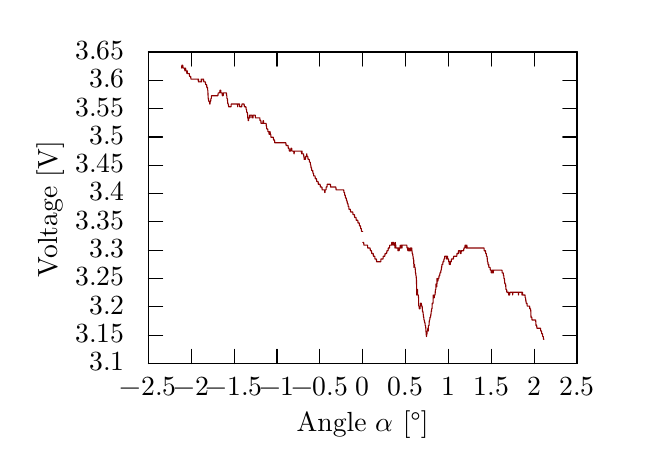
\begin{tikzpicture}[gnuplot]
%% generated with GNUPLOT 5.2p5a (Gentoo revision r0) (Lua 5.1; terminal rev. 99 , script rev. 107)
%% Mi 01 Mai 2019 12:59:13 CEST
\path (0.000,0.000) rectangle (7.500,5.250);
\gpcolor{color=gp lt color border}
\gpsetlinetype{gp lt border}
\gpsetdashtype{gp dt solid}
\gpsetlinewidth{1.00}
\draw[gp path] (1.504,0.985)--(1.684,0.985);
\draw[gp path] (6.947,0.985)--(6.767,0.985);
\node[gp node right] at (1.320,0.985) {$3.1$};
\draw[gp path] (1.504,1.345)--(1.684,1.345);
\draw[gp path] (6.947,1.345)--(6.767,1.345);
\node[gp node right] at (1.320,1.345) {$3.15$};
\draw[gp path] (1.504,1.704)--(1.684,1.704);
\draw[gp path] (6.947,1.704)--(6.767,1.704);
\node[gp node right] at (1.320,1.704) {$3.2$};
\draw[gp path] (1.504,2.064)--(1.684,2.064);
\draw[gp path] (6.947,2.064)--(6.767,2.064);
\node[gp node right] at (1.320,2.064) {$3.25$};
\draw[gp path] (1.504,2.424)--(1.684,2.424);
\draw[gp path] (6.947,2.424)--(6.767,2.424);
\node[gp node right] at (1.320,2.424) {$3.3$};
\draw[gp path] (1.504,2.783)--(1.684,2.783);
\draw[gp path] (6.947,2.783)--(6.767,2.783);
\node[gp node right] at (1.320,2.783) {$3.35$};
\draw[gp path] (1.504,3.143)--(1.684,3.143);
\draw[gp path] (6.947,3.143)--(6.767,3.143);
\node[gp node right] at (1.320,3.143) {$3.4$};
\draw[gp path] (1.504,3.502)--(1.684,3.502);
\draw[gp path] (6.947,3.502)--(6.767,3.502);
\node[gp node right] at (1.320,3.502) {$3.45$};
\draw[gp path] (1.504,3.862)--(1.684,3.862);
\draw[gp path] (6.947,3.862)--(6.767,3.862);
\node[gp node right] at (1.320,3.862) {$3.5$};
\draw[gp path] (1.504,4.222)--(1.684,4.222);
\draw[gp path] (6.947,4.222)--(6.767,4.222);
\node[gp node right] at (1.320,4.222) {$3.55$};
\draw[gp path] (1.504,4.581)--(1.684,4.581);
\draw[gp path] (6.947,4.581)--(6.767,4.581);
\node[gp node right] at (1.320,4.581) {$3.6$};
\draw[gp path] (1.504,4.941)--(1.684,4.941);
\draw[gp path] (6.947,4.941)--(6.767,4.941);
\node[gp node right] at (1.320,4.941) {$3.65$};
\draw[gp path] (1.504,0.985)--(1.504,1.165);
\draw[gp path] (1.504,4.941)--(1.504,4.761);
\node[gp node center] at (1.504,0.677) {$-2.5$};
\draw[gp path] (2.048,0.985)--(2.048,1.165);
\draw[gp path] (2.048,4.941)--(2.048,4.761);
\node[gp node center] at (2.048,0.677) {$-2$};
\draw[gp path] (2.593,0.985)--(2.593,1.165);
\draw[gp path] (2.593,4.941)--(2.593,4.761);
\node[gp node center] at (2.593,0.677) {$-1.5$};
\draw[gp path] (3.137,0.985)--(3.137,1.165);
\draw[gp path] (3.137,4.941)--(3.137,4.761);
\node[gp node center] at (3.137,0.677) {$-1$};
\draw[gp path] (3.681,0.985)--(3.681,1.165);
\draw[gp path] (3.681,4.941)--(3.681,4.761);
\node[gp node center] at (3.681,0.677) {$-0.5$};
\draw[gp path] (4.226,0.985)--(4.226,1.165);
\draw[gp path] (4.226,4.941)--(4.226,4.761);
\node[gp node center] at (4.226,0.677) {$0$};
\draw[gp path] (4.770,0.985)--(4.770,1.165);
\draw[gp path] (4.770,4.941)--(4.770,4.761);
\node[gp node center] at (4.770,0.677) {$0.5$};
\draw[gp path] (5.314,0.985)--(5.314,1.165);
\draw[gp path] (5.314,4.941)--(5.314,4.761);
\node[gp node center] at (5.314,0.677) {$1$};
\draw[gp path] (5.858,0.985)--(5.858,1.165);
\draw[gp path] (5.858,4.941)--(5.858,4.761);
\node[gp node center] at (5.858,0.677) {$1.5$};
\draw[gp path] (6.403,0.985)--(6.403,1.165);
\draw[gp path] (6.403,4.941)--(6.403,4.761);
\node[gp node center] at (6.403,0.677) {$2$};
\draw[gp path] (6.947,0.985)--(6.947,1.165);
\draw[gp path] (6.947,4.941)--(6.947,4.761);
\node[gp node center] at (6.947,0.677) {$2.5$};
\draw[gp path] (1.504,4.941)--(1.504,0.985)--(6.947,0.985)--(6.947,4.941)--cycle;
\node[gp node center,rotate=-270] at (0.276,2.963) {Voltage [V]};
\node[gp node center] at (4.225,0.215) {Angle $\alpha$ [°]};
\gpcolor{rgb color={0.545,0.000,0.000}}
\draw[gp path] (4.226,2.523)--(4.228,2.523)--(4.231,2.523)--(4.233,2.523)--(4.236,2.523)%
  --(4.238,2.523)--(4.241,2.488)--(4.243,2.488)--(4.246,2.488)--(4.249,2.488)--(4.251,2.488)%
  --(4.254,2.488)--(4.256,2.488)--(4.259,2.488)--(4.261,2.488)--(4.264,2.488)--(4.266,2.488)%
  --(4.269,2.488)--(4.272,2.488)--(4.274,2.488)--(4.277,2.488)--(4.279,2.488)--(4.282,2.488)%
  --(4.284,2.488)--(4.287,2.488)--(4.290,2.452)--(4.292,2.452)--(4.295,2.452)--(4.297,2.452)%
  --(4.300,2.452)--(4.302,2.452)--(4.305,2.452)--(4.307,2.452)--(4.310,2.452)--(4.313,2.452)%
  --(4.315,2.452)--(4.318,2.452)--(4.320,2.452)--(4.323,2.417)--(4.325,2.417)--(4.328,2.417)%
  --(4.330,2.417)--(4.333,2.417)--(4.336,2.417)--(4.338,2.417)--(4.341,2.382)--(4.343,2.382)%
  --(4.346,2.382)--(4.348,2.382)--(4.351,2.382)--(4.354,2.382)--(4.356,2.382)--(4.359,2.382)%
  --(4.361,2.347)--(4.364,2.347)--(4.366,2.347)--(4.369,2.347)--(4.371,2.347)--(4.374,2.347)%
  --(4.377,2.347)--(4.379,2.347)--(4.382,2.312)--(4.384,2.312)--(4.387,2.312)--(4.389,2.312)%
  --(4.392,2.312)--(4.394,2.312)--(4.397,2.312)--(4.400,2.312)--(4.402,2.277)--(4.405,2.277)%
  --(4.407,2.277)--(4.410,2.277)--(4.412,2.277)--(4.415,2.277)--(4.418,2.277)--(4.420,2.277)%
  --(4.423,2.277)--(4.425,2.277)--(4.428,2.277)--(4.430,2.277)--(4.433,2.277)--(4.435,2.277)%
  --(4.438,2.277)--(4.441,2.277)--(4.443,2.277)--(4.446,2.277)--(4.448,2.277)--(4.451,2.277)%
  --(4.453,2.277)--(4.456,2.277)--(4.458,2.312)--(4.461,2.312)--(4.464,2.312)--(4.466,2.312)%
  --(4.469,2.312)--(4.471,2.312)--(4.474,2.312)--(4.476,2.312)--(4.479,2.312)--(4.482,2.312)%
  --(4.484,2.312)--(4.487,2.347)--(4.489,2.347)--(4.492,2.347)--(4.494,2.347)--(4.497,2.347)%
  --(4.499,2.347)--(4.502,2.347)--(4.505,2.347)--(4.507,2.347)--(4.510,2.382)--(4.512,2.382)%
  --(4.515,2.382)--(4.517,2.382)--(4.520,2.382)--(4.523,2.382)--(4.525,2.382)--(4.528,2.382)%
  --(4.530,2.382)--(4.533,2.417)--(4.535,2.417)--(4.538,2.417)--(4.540,2.417)--(4.543,2.417)%
  --(4.546,2.417)--(4.548,2.417)--(4.551,2.452)--(4.553,2.452)--(4.556,2.452)--(4.558,2.452)%
  --(4.561,2.452)--(4.563,2.452)--(4.566,2.452)--(4.569,2.488)--(4.571,2.488)--(4.574,2.488)%
  --(4.576,2.488)--(4.579,2.488)--(4.581,2.488)--(4.584,2.488)--(4.587,2.488)--(4.589,2.488)%
  --(4.592,2.488)--(4.594,2.523)--(4.597,2.523)--(4.599,2.523)--(4.602,2.523)--(4.604,2.523)%
  --(4.607,2.523)--(4.610,2.488)--(4.612,2.523)--(4.615,2.523)--(4.617,2.523)--(4.620,2.523)%
  --(4.622,2.488)--(4.625,2.488)--(4.627,2.488)--(4.630,2.488)--(4.633,2.488)--(4.635,2.452)%
  --(4.638,2.452)--(4.640,2.523)--(4.643,2.488)--(4.645,2.488)--(4.648,2.452)--(4.651,2.452)%
  --(4.653,2.452)--(4.656,2.452)--(4.658,2.452)--(4.661,2.452)--(4.663,2.452)--(4.666,2.452)%
  --(4.668,2.452)--(4.671,2.452)--(4.674,2.417)--(4.676,2.452)--(4.679,2.452)--(4.681,2.452)%
  --(4.684,2.452)--(4.686,2.417)--(4.689,2.417)--(4.691,2.452)--(4.694,2.452)--(4.697,2.452)%
  --(4.699,2.452)--(4.702,2.488)--(4.704,2.452)--(4.707,2.452)--(4.709,2.452)--(4.712,2.452)%
  --(4.715,2.488)--(4.717,2.488)--(4.720,2.488)--(4.722,2.488)--(4.725,2.452)--(4.727,2.488)%
  --(4.730,2.488)--(4.732,2.488)--(4.735,2.488)--(4.738,2.488)--(4.740,2.488)--(4.743,2.488)%
  --(4.745,2.488)--(4.748,2.488)--(4.750,2.488)--(4.753,2.488)--(4.756,2.488)--(4.758,2.488)%
  --(4.761,2.488)--(4.763,2.488)--(4.766,2.488)--(4.768,2.488)--(4.771,2.488)--(4.773,2.488)%
  --(4.776,2.488)--(4.779,2.488)--(4.781,2.488)--(4.784,2.488)--(4.786,2.488)--(4.789,2.452)%
  --(4.791,2.452)--(4.794,2.452)--(4.796,2.452)--(4.799,2.417)--(4.802,2.452)--(4.804,2.452)%
  --(4.807,2.417)--(4.809,2.417)--(4.812,2.452)--(4.814,2.417)--(4.817,2.417)--(4.820,2.417)%
  --(4.822,2.417)--(4.825,2.417)--(4.827,2.417)--(4.830,2.452)--(4.832,2.417)--(4.835,2.417)%
  --(4.837,2.452)--(4.840,2.452)--(4.843,2.417)--(4.845,2.417)--(4.848,2.452)--(4.850,2.417)%
  --(4.853,2.417)--(4.855,2.382)--(4.858,2.382)--(4.860,2.382)--(4.863,2.347)--(4.866,2.347)%
  --(4.868,2.312)--(4.871,2.312)--(4.873,2.312)--(4.876,2.206)--(4.878,2.206)--(4.881,2.242)%
  --(4.884,2.242)--(4.886,2.206)--(4.889,2.206)--(4.891,2.206)--(4.894,2.171)--(4.896,2.136)%
  --(4.899,2.136)--(4.901,2.101)--(4.904,2.101)--(4.907,2.065)--(4.909,2.031)--(4.912,1.855)%
  --(4.914,1.925)--(4.917,1.925)--(4.919,1.925)--(4.922,1.925)--(4.924,1.855)--(4.927,1.855)%
  --(4.930,1.855)--(4.932,1.855)--(4.935,1.819)--(4.937,1.714)--(4.940,1.714)--(4.942,1.714)%
  --(4.945,1.679)--(4.948,1.679)--(4.950,1.679)--(4.953,1.679)--(4.955,1.714)--(4.958,1.714)%
  --(4.960,1.750)--(4.963,1.750)--(4.965,1.750)--(4.968,1.750)--(4.971,1.750)--(4.973,1.714)%
  --(4.976,1.714)--(4.978,1.714)--(4.981,1.714)--(4.983,1.679)--(4.986,1.644)--(4.988,1.644)%
  --(4.991,1.644)--(4.994,1.609)--(4.996,1.609)--(4.999,1.573)--(5.001,1.573)--(5.004,1.538)%
  --(5.006,1.538)--(5.009,1.538)--(5.012,1.503)--(5.014,1.503)--(5.017,1.503)--(5.019,1.468)%
  --(5.022,1.468)--(5.024,1.468)--(5.027,1.433)--(5.029,1.398)--(5.032,1.363)--(5.035,1.327)%
  --(5.037,1.327)--(5.040,1.363)--(5.042,1.363)--(5.045,1.398)--(5.047,1.398)--(5.050,1.398)%
  --(5.053,1.433)--(5.055,1.433)--(5.058,1.398)--(5.060,1.468)--(5.063,1.468)--(5.065,1.468)%
  --(5.068,1.468)--(5.070,1.503)--(5.073,1.538)--(5.076,1.538)--(5.078,1.538)--(5.081,1.573)%
  --(5.083,1.573)--(5.086,1.573)--(5.088,1.573)--(5.091,1.609)--(5.093,1.609)--(5.096,1.644)%
  --(5.099,1.644)--(5.101,1.679)--(5.104,1.679)--(5.106,1.679)--(5.109,1.750)--(5.111,1.750)%
  --(5.114,1.750)--(5.117,1.750)--(5.119,1.750)--(5.122,1.855)--(5.124,1.819)--(5.127,1.819)%
  --(5.129,1.819)--(5.132,1.819)--(5.134,1.819)--(5.137,1.855)--(5.140,1.855)--(5.142,1.855)%
  --(5.145,1.855)--(5.147,1.890)--(5.150,1.925)--(5.152,1.925)--(5.155,1.925)--(5.157,1.996)%
  --(5.160,1.960)--(5.163,1.960)--(5.165,1.960)--(5.168,1.960)--(5.170,2.065)--(5.173,2.065)%
  --(5.175,2.031)--(5.178,2.031)--(5.181,2.031)--(5.183,2.065)--(5.186,2.065)--(5.188,2.065)%
  --(5.191,2.065)--(5.193,2.065)--(5.196,2.101)--(5.198,2.101)--(5.201,2.101)--(5.204,2.101)%
  --(5.206,2.136)--(5.209,2.136)--(5.211,2.136)--(5.214,2.136)--(5.216,2.136)--(5.219,2.171)%
  --(5.221,2.171)--(5.224,2.171)--(5.227,2.206)--(5.229,2.206)--(5.232,2.242)--(5.234,2.242)%
  --(5.237,2.242)--(5.239,2.242)--(5.242,2.242)--(5.245,2.277)--(5.247,2.277)--(5.250,2.277)%
  --(5.252,2.277)--(5.255,2.277)--(5.257,2.312)--(5.260,2.312)--(5.262,2.312)--(5.265,2.312)%
  --(5.268,2.347)--(5.270,2.347)--(5.273,2.347)--(5.275,2.347)--(5.278,2.347)--(5.280,2.347)%
  --(5.283,2.347)--(5.286,2.347)--(5.288,2.347)--(5.291,2.312)--(5.293,2.347)--(5.296,2.312)%
  --(5.298,2.312)--(5.301,2.347)--(5.303,2.347)--(5.306,2.312)--(5.309,2.312)--(5.311,2.312)%
  --(5.314,2.312)--(5.316,2.312)--(5.319,2.277)--(5.321,2.277)--(5.324,2.277)--(5.326,2.242)%
  --(5.329,2.277)--(5.332,2.277)--(5.334,2.277)--(5.337,2.242)--(5.339,2.277)--(5.342,2.277)%
  --(5.344,2.277)--(5.347,2.277)--(5.350,2.277)--(5.352,2.312)--(5.355,2.312)--(5.357,2.312)%
  --(5.360,2.312)--(5.362,2.312)--(5.365,2.312)--(5.367,2.312)--(5.370,2.312)--(5.373,2.312)%
  --(5.375,2.312)--(5.378,2.312)--(5.380,2.347)--(5.383,2.347)--(5.385,2.347)--(5.388,2.347)%
  --(5.390,2.347)--(5.393,2.347)--(5.396,2.347)--(5.398,2.347)--(5.401,2.347)--(5.403,2.347)%
  --(5.406,2.347)--(5.408,2.347)--(5.411,2.347)--(5.414,2.347)--(5.416,2.347)--(5.419,2.347)%
  --(5.421,2.347)--(5.424,2.382)--(5.426,2.382)--(5.429,2.382)--(5.431,2.382)--(5.434,2.382)%
  --(5.437,2.382)--(5.439,2.382)--(5.442,2.417)--(5.444,2.382)--(5.447,2.417)--(5.449,2.417)%
  --(5.452,2.417)--(5.454,2.417)--(5.457,2.417)--(5.460,2.417)--(5.462,2.417)--(5.465,2.417)%
  --(5.467,2.382)--(5.470,2.382)--(5.472,2.382)--(5.475,2.382)--(5.478,2.417)--(5.480,2.417)%
  --(5.483,2.417)--(5.485,2.417)--(5.488,2.417)--(5.490,2.417)--(5.493,2.417)--(5.495,2.417)%
  --(5.498,2.417)--(5.501,2.417)--(5.503,2.417)--(5.506,2.417)--(5.508,2.417)--(5.511,2.452)%
  --(5.513,2.452)--(5.516,2.452)--(5.518,2.452)--(5.521,2.452)--(5.524,2.452)--(5.526,2.488)%
  --(5.529,2.488)--(5.531,2.488)--(5.534,2.488)--(5.536,2.488)--(5.539,2.452)--(5.542,2.452)%
  --(5.544,2.452)--(5.547,2.452)--(5.549,2.488)--(5.552,2.452)--(5.554,2.452)--(5.557,2.452)%
  --(5.559,2.452)--(5.562,2.452)--(5.565,2.452)--(5.567,2.452)--(5.570,2.452)--(5.572,2.452)%
  --(5.575,2.452)--(5.577,2.452)--(5.580,2.452)--(5.583,2.452)--(5.585,2.452)--(5.588,2.452)%
  --(5.590,2.452)--(5.593,2.452)--(5.595,2.452)--(5.598,2.452)--(5.600,2.452)--(5.603,2.452)%
  --(5.606,2.452)--(5.608,2.452)--(5.611,2.452)--(5.613,2.452)--(5.616,2.452)--(5.618,2.452)%
  --(5.621,2.452)--(5.623,2.452)--(5.626,2.452)--(5.629,2.452)--(5.631,2.452)--(5.634,2.452)%
  --(5.636,2.452)--(5.639,2.452)--(5.641,2.452)--(5.644,2.452)--(5.647,2.452)--(5.649,2.452)%
  --(5.652,2.452)--(5.654,2.452)--(5.657,2.452)--(5.659,2.452)--(5.662,2.452)--(5.664,2.452)%
  --(5.667,2.452)--(5.670,2.452)--(5.672,2.452)--(5.675,2.452)--(5.677,2.452)--(5.680,2.452)%
  --(5.682,2.452)--(5.685,2.452)--(5.687,2.452)--(5.690,2.452)--(5.693,2.452)--(5.695,2.452)%
  --(5.698,2.452)--(5.700,2.452)--(5.703,2.452)--(5.705,2.452)--(5.708,2.452)--(5.711,2.452)%
  --(5.713,2.452)--(5.716,2.452)--(5.718,2.452)--(5.721,2.452)--(5.723,2.452)--(5.726,2.452)%
  --(5.728,2.452)--(5.731,2.452)--(5.734,2.452)--(5.736,2.452)--(5.739,2.452)--(5.741,2.452)%
  --(5.744,2.452)--(5.746,2.452)--(5.749,2.452)--(5.751,2.452)--(5.754,2.452)--(5.757,2.452)%
  --(5.759,2.452)--(5.762,2.452)--(5.764,2.452)--(5.767,2.452)--(5.769,2.417)--(5.772,2.417)%
  --(5.775,2.417)--(5.777,2.417)--(5.780,2.417)--(5.782,2.417)--(5.785,2.417)--(5.787,2.382)%
  --(5.790,2.382)--(5.792,2.382)--(5.795,2.382)--(5.798,2.347)--(5.800,2.347)--(5.803,2.347)%
  --(5.805,2.347)--(5.808,2.312)--(5.810,2.277)--(5.813,2.277)--(5.816,2.277)--(5.818,2.242)%
  --(5.821,2.242)--(5.823,2.242)--(5.826,2.242)--(5.828,2.206)--(5.831,2.206)--(5.833,2.206)%
  --(5.836,2.206)--(5.839,2.206)--(5.841,2.206)--(5.844,2.206)--(5.846,2.171)--(5.849,2.171)%
  --(5.851,2.171)--(5.854,2.171)--(5.856,2.171)--(5.859,2.136)--(5.862,2.136)--(5.864,2.136)%
  --(5.867,2.136)--(5.869,2.171)--(5.872,2.136)--(5.874,2.136)--(5.877,2.136)--(5.880,2.171)%
  --(5.882,2.171)--(5.885,2.136)--(5.887,2.171)--(5.890,2.171)--(5.892,2.171)--(5.895,2.171)%
  --(5.897,2.171)--(5.900,2.171)--(5.903,2.171)--(5.905,2.171)--(5.908,2.171)--(5.910,2.171)%
  --(5.913,2.171)--(5.915,2.171)--(5.918,2.171)--(5.920,2.171)--(5.923,2.171)--(5.926,2.171)%
  --(5.928,2.171)--(5.931,2.171)--(5.933,2.171)--(5.936,2.171)--(5.938,2.171)--(5.941,2.171)%
  --(5.944,2.171)--(5.946,2.171)--(5.949,2.171)--(5.951,2.171)--(5.954,2.171)--(5.956,2.171)%
  --(5.959,2.171)--(5.961,2.171)--(5.964,2.171)--(5.967,2.171)--(5.969,2.171)--(5.972,2.171)%
  --(5.974,2.171)--(5.977,2.171)--(5.979,2.171)--(5.982,2.171)--(5.984,2.171)--(5.987,2.171)%
  --(5.990,2.171)--(5.992,2.171)--(5.995,2.171)--(5.997,2.136)--(6.000,2.136)--(6.002,2.136)%
  --(6.005,2.136)--(6.008,2.136)--(6.010,2.136)--(6.013,2.101)--(6.015,2.101)--(6.018,2.101)%
  --(6.020,2.065)--(6.023,2.065)--(6.025,2.065)--(6.028,2.031)--(6.031,1.996)--(6.033,1.996)%
  --(6.036,1.996)--(6.038,1.996)--(6.041,1.996)--(6.043,1.960)--(6.046,1.925)--(6.048,1.925)%
  --(6.051,1.925)--(6.054,1.925)--(6.056,1.890)--(6.059,1.890)--(6.061,1.890)--(6.064,1.890)%
  --(6.066,1.890)--(6.069,1.890)--(6.072,1.890)--(6.074,1.890)--(6.077,1.890)--(6.079,1.855)%
  --(6.082,1.855)--(6.084,1.855)--(6.087,1.855)--(6.089,1.855)--(6.092,1.855)--(6.095,1.890)%
  --(6.097,1.890)--(6.100,1.890)--(6.102,1.890)--(6.105,1.890)--(6.107,1.890)--(6.110,1.890)%
  --(6.113,1.890)--(6.115,1.890)--(6.118,1.890)--(6.120,1.890)--(6.123,1.890)--(6.125,1.890)%
  --(6.128,1.890)--(6.130,1.855)--(6.133,1.890)--(6.136,1.890)--(6.138,1.890)--(6.141,1.890)%
  --(6.143,1.890)--(6.146,1.890)--(6.148,1.890)--(6.151,1.890)--(6.153,1.890)--(6.156,1.890)%
  --(6.159,1.890)--(6.161,1.890)--(6.164,1.890)--(6.166,1.890)--(6.169,1.890)--(6.171,1.890)%
  --(6.174,1.890)--(6.177,1.890)--(6.179,1.890)--(6.182,1.890)--(6.184,1.890)--(6.187,1.890)%
  --(6.189,1.890)--(6.192,1.890)--(6.194,1.890)--(6.197,1.890)--(6.200,1.890)--(6.202,1.890)%
  --(6.205,1.855)--(6.207,1.890)--(6.210,1.890)--(6.212,1.890)--(6.215,1.890)--(6.217,1.890)%
  --(6.220,1.890)--(6.223,1.890)--(6.225,1.890)--(6.228,1.890)--(6.230,1.890)--(6.233,1.890)%
  --(6.235,1.890)--(6.238,1.890)--(6.241,1.890)--(6.243,1.890)--(6.246,1.890)--(6.248,1.855)%
  --(6.251,1.855)--(6.253,1.890)--(6.256,1.890)--(6.258,1.855)--(6.261,1.855)--(6.264,1.855)%
  --(6.266,1.855)--(6.269,1.855)--(6.271,1.855)--(6.274,1.855)--(6.276,1.855)--(6.279,1.855)%
  --(6.281,1.855)--(6.284,1.855)--(6.287,1.855)--(6.289,1.819)--(6.292,1.819)--(6.294,1.819)%
  --(6.297,1.784)--(6.299,1.784)--(6.302,1.750)--(6.305,1.750)--(6.307,1.750)--(6.310,1.750)%
  --(6.312,1.750)--(6.315,1.714)--(6.317,1.714)--(6.320,1.714)--(6.322,1.714)--(6.325,1.714)%
  --(6.328,1.714)--(6.330,1.714)--(6.333,1.714)--(6.335,1.714)--(6.338,1.714)--(6.340,1.714)%
  --(6.343,1.714)--(6.346,1.714)--(6.348,1.679)--(6.351,1.679)--(6.353,1.679)--(6.356,1.679)%
  --(6.358,1.679)--(6.361,1.644)--(6.363,1.573)--(6.366,1.573)--(6.369,1.573)--(6.371,1.573)%
  --(6.374,1.573)--(6.376,1.538)--(6.379,1.538)--(6.381,1.538)--(6.384,1.538)--(6.386,1.538)%
  --(6.389,1.538)--(6.392,1.538)--(6.394,1.538)--(6.397,1.538)--(6.399,1.538)--(6.402,1.538)%
  --(6.404,1.538)--(6.407,1.538)--(6.410,1.538)--(6.412,1.538)--(6.415,1.538)--(6.417,1.538)%
  --(6.420,1.538)--(6.422,1.538)--(6.425,1.503)--(6.427,1.468)--(6.430,1.468)--(6.433,1.468)%
  --(6.435,1.468)--(6.438,1.433)--(6.440,1.433)--(6.443,1.433)--(6.445,1.433)--(6.448,1.433)%
  --(6.450,1.433)--(6.453,1.433)--(6.456,1.433)--(6.458,1.433)--(6.461,1.433)--(6.463,1.433)%
  --(6.466,1.433)--(6.468,1.433)--(6.471,1.433)--(6.474,1.433)--(6.476,1.433)--(6.479,1.433)%
  --(6.481,1.433)--(6.484,1.433)--(6.486,1.398)--(6.489,1.398)--(6.491,1.398)--(6.494,1.398)%
  --(6.497,1.398)--(6.499,1.363)--(6.502,1.363)--(6.504,1.363)--(6.507,1.363)--(6.509,1.363)%
  --(6.512,1.327)--(6.514,1.327)--(6.517,1.327)--(6.520,1.327)--(6.522,1.292)--(6.525,1.292)%
  --(6.527,1.292);
\draw[gp path] (4.226,2.663)--(4.223,2.663)--(4.220,2.663)--(4.218,2.663)--(4.215,2.663)%
  --(4.213,2.663)--(4.210,2.663)--(4.208,2.698)--(4.205,2.698)--(4.202,2.698)--(4.200,2.698)%
  --(4.197,2.734)--(4.195,2.734)--(4.192,2.734)--(4.190,2.734)--(4.187,2.734)--(4.185,2.734)%
  --(4.182,2.769)--(4.179,2.769)--(4.177,2.769)--(4.174,2.769)--(4.172,2.769)--(4.169,2.769)%
  --(4.167,2.769)--(4.164,2.804)--(4.161,2.804)--(4.159,2.804)--(4.156,2.804)--(4.154,2.804)%
  --(4.151,2.804)--(4.149,2.804)--(4.146,2.804)--(4.144,2.804)--(4.141,2.839)--(4.138,2.839)%
  --(4.136,2.839)--(4.133,2.839)--(4.131,2.839)--(4.128,2.839)--(4.126,2.839)--(4.123,2.839)%
  --(4.121,2.875)--(4.118,2.875)--(4.115,2.875)--(4.113,2.875)--(4.110,2.875)--(4.108,2.875)%
  --(4.105,2.875)--(4.103,2.875)--(4.100,2.909)--(4.097,2.909)--(4.095,2.909)--(4.092,2.909)%
  --(4.090,2.909)--(4.087,2.909)--(4.085,2.909)--(4.082,2.909)--(4.080,2.909)--(4.077,2.909)%
  --(4.074,2.909)--(4.072,2.909)--(4.069,2.944)--(4.067,2.944)--(4.064,2.944)--(4.062,2.944)%
  --(4.059,2.944)--(4.057,2.944)--(4.054,2.944)--(4.051,2.944)--(4.049,2.980)--(4.046,2.980)%
  --(4.044,2.980)--(4.041,2.980)--(4.039,3.015)--(4.036,3.015)--(4.033,3.015)--(4.031,3.015)%
  --(4.028,3.050)--(4.026,3.050)--(4.023,3.050)--(4.021,3.050)--(4.018,3.085)--(4.016,3.085)%
  --(4.013,3.085)--(4.010,3.085)--(4.008,3.085)--(4.005,3.121)--(4.003,3.121)--(4.000,3.121)%
  --(3.998,3.121)--(3.995,3.156)--(3.993,3.156)--(3.990,3.156)--(3.987,3.156)--(3.985,3.190)%
  --(3.982,3.190)--(3.980,3.190)--(3.977,3.190)--(3.975,3.190)--(3.972,3.190)--(3.969,3.190)%
  --(3.967,3.190)--(3.964,3.190)--(3.962,3.190)--(3.959,3.190)--(3.957,3.190)--(3.954,3.190)%
  --(3.952,3.190)--(3.949,3.190)--(3.946,3.190)--(3.944,3.190)--(3.941,3.190)--(3.939,3.190)%
  --(3.936,3.190)--(3.934,3.190)--(3.931,3.190)--(3.928,3.190)--(3.926,3.190)--(3.923,3.190)%
  --(3.921,3.190)--(3.918,3.190)--(3.916,3.190)--(3.913,3.190)--(3.911,3.190)--(3.908,3.190)%
  --(3.905,3.190)--(3.903,3.190)--(3.900,3.190)--(3.898,3.190)--(3.895,3.190)--(3.893,3.190)%
  --(3.890,3.190)--(3.888,3.190)--(3.885,3.226)--(3.882,3.226)--(3.880,3.226)--(3.877,3.226)%
  --(3.875,3.226)--(3.872,3.226)--(3.870,3.226)--(3.867,3.226)--(3.864,3.226)--(3.862,3.226)%
  --(3.859,3.226)--(3.857,3.226)--(3.854,3.226)--(3.852,3.226)--(3.849,3.226)--(3.847,3.226)%
  --(3.844,3.226)--(3.841,3.226)--(3.839,3.226)--(3.836,3.226)--(3.834,3.226)--(3.831,3.226)%
  --(3.829,3.226)--(3.826,3.226)--(3.824,3.226)--(3.821,3.226)--(3.818,3.226)--(3.816,3.261)%
  --(3.813,3.261)--(3.811,3.261)--(3.808,3.261)--(3.806,3.261)--(3.803,3.261)--(3.800,3.261)%
  --(3.798,3.261)--(3.795,3.261)--(3.793,3.261)--(3.790,3.261)--(3.788,3.261)--(3.785,3.261)%
  --(3.783,3.261)--(3.780,3.261)--(3.777,3.261)--(3.775,3.261)--(3.772,3.226)--(3.770,3.226)%
  --(3.767,3.226)--(3.765,3.226)--(3.762,3.226)--(3.760,3.190)--(3.757,3.190)--(3.754,3.190)%
  --(3.752,3.190)--(3.749,3.190)--(3.747,3.156)--(3.744,3.156)--(3.742,3.190)--(3.739,3.190)%
  --(3.736,3.190)--(3.734,3.190)--(3.731,3.190)--(3.729,3.190)--(3.726,3.190)--(3.724,3.190)%
  --(3.721,3.190)--(3.719,3.190)--(3.716,3.190)--(3.713,3.190)--(3.711,3.190)--(3.708,3.226)%
  --(3.706,3.226)--(3.703,3.226)--(3.701,3.226)--(3.698,3.226)--(3.695,3.226)--(3.693,3.226)%
  --(3.690,3.226)--(3.688,3.226)--(3.685,3.261)--(3.683,3.261)--(3.680,3.261)--(3.678,3.261)%
  --(3.675,3.261)--(3.672,3.261)--(3.670,3.261)--(3.667,3.261)--(3.665,3.261)--(3.662,3.261)%
  --(3.660,3.296)--(3.657,3.296)--(3.655,3.296)--(3.652,3.296)--(3.649,3.296)--(3.647,3.296)%
  --(3.644,3.296)--(3.642,3.296)--(3.639,3.331)--(3.637,3.331)--(3.634,3.331)--(3.631,3.331)%
  --(3.629,3.331)--(3.626,3.331)--(3.624,3.331)--(3.621,3.367)--(3.619,3.367)--(3.616,3.367)%
  --(3.614,3.367)--(3.611,3.367)--(3.608,3.367)--(3.606,3.367)--(3.603,3.367)--(3.601,3.402)%
  --(3.598,3.402)--(3.596,3.402)--(3.593,3.402)--(3.591,3.437)--(3.588,3.437)--(3.585,3.437)%
  --(3.583,3.437)--(3.580,3.437)--(3.578,3.437)--(3.575,3.472)--(3.573,3.472)--(3.570,3.472)%
  --(3.567,3.507)--(3.565,3.507)--(3.562,3.507)--(3.560,3.542)--(3.557,3.542)--(3.555,3.542)%
  --(3.552,3.542)--(3.550,3.542)--(3.547,3.577)--(3.544,3.577)--(3.542,3.577)--(3.539,3.577)%
  --(3.537,3.577)--(3.534,3.577)--(3.532,3.577)--(3.529,3.613)--(3.527,3.613)--(3.524,3.613)%
  --(3.521,3.613)--(3.519,3.613)--(3.516,3.648)--(3.514,3.648)--(3.511,3.613)--(3.509,3.613)%
  --(3.506,3.613)--(3.503,3.613)--(3.501,3.613)--(3.498,3.577)--(3.496,3.577)--(3.493,3.577)%
  --(3.491,3.577)--(3.488,3.577)--(3.486,3.577)--(3.483,3.577)--(3.480,3.613)--(3.478,3.613)%
  --(3.475,3.648)--(3.473,3.648)--(3.470,3.648)--(3.468,3.648)--(3.465,3.648)--(3.463,3.648)%
  --(3.460,3.648)--(3.457,3.648)--(3.455,3.683)--(3.452,3.683)--(3.450,3.648)--(3.447,3.683)%
  --(3.445,3.683)--(3.442,3.683)--(3.439,3.683)--(3.437,3.683)--(3.434,3.683)--(3.432,3.683)%
  --(3.429,3.683)--(3.427,3.683)--(3.424,3.683)--(3.422,3.683)--(3.419,3.683)--(3.416,3.683)%
  --(3.414,3.683)--(3.411,3.683)--(3.409,3.683)--(3.406,3.683)--(3.404,3.683)--(3.401,3.683)%
  --(3.398,3.683)--(3.396,3.683)--(3.393,3.683)--(3.391,3.683)--(3.388,3.683)--(3.386,3.683)%
  --(3.383,3.683)--(3.381,3.683)--(3.378,3.683)--(3.375,3.683)--(3.373,3.683)--(3.370,3.683)%
  --(3.368,3.683)--(3.365,3.683)--(3.363,3.683)--(3.360,3.683)--(3.358,3.683)--(3.355,3.648)%
  --(3.352,3.648)--(3.350,3.683)--(3.347,3.683)--(3.345,3.683)--(3.342,3.683)--(3.340,3.683)%
  --(3.337,3.683)--(3.334,3.683)--(3.332,3.683)--(3.329,3.683)--(3.327,3.683)--(3.324,3.718)%
  --(3.322,3.718)--(3.319,3.718)--(3.317,3.718)--(3.314,3.718)--(3.311,3.683)--(3.309,3.683)%
  --(3.306,3.683)--(3.304,3.683)--(3.301,3.683)--(3.299,3.683)--(3.296,3.683)--(3.294,3.683)%
  --(3.291,3.718)--(3.288,3.718)--(3.286,3.718)--(3.283,3.718)--(3.281,3.718)--(3.278,3.753)%
  --(3.276,3.753)--(3.273,3.753)--(3.270,3.753)--(3.268,3.753)--(3.265,3.753)--(3.263,3.753)%
  --(3.260,3.753)--(3.258,3.753)--(3.255,3.753)--(3.253,3.753)--(3.250,3.788)--(3.247,3.788)%
  --(3.245,3.788)--(3.242,3.788)--(3.240,3.788)--(3.237,3.788)--(3.235,3.788)--(3.232,3.788)%
  --(3.230,3.788)--(3.227,3.788)--(3.224,3.788)--(3.222,3.788)--(3.219,3.788)--(3.217,3.788)%
  --(3.214,3.788)--(3.212,3.788)--(3.209,3.788)--(3.206,3.788)--(3.204,3.788)--(3.201,3.788)%
  --(3.199,3.788)--(3.196,3.788)--(3.194,3.788)--(3.191,3.788)--(3.189,3.788)--(3.186,3.788)%
  --(3.183,3.788)--(3.181,3.788)--(3.178,3.788)--(3.176,3.788)--(3.173,3.788)--(3.171,3.788)%
  --(3.168,3.788)--(3.165,3.788)--(3.163,3.788)--(3.160,3.788)--(3.158,3.788)--(3.155,3.788)%
  --(3.153,3.788)--(3.150,3.788)--(3.148,3.788)--(3.145,3.788)--(3.142,3.788)--(3.140,3.788)%
  --(3.137,3.788)--(3.135,3.788)--(3.132,3.788)--(3.130,3.788)--(3.127,3.788)--(3.125,3.788)%
  --(3.122,3.788)--(3.119,3.788)--(3.117,3.788)--(3.114,3.788)--(3.112,3.788)--(3.109,3.788)%
  --(3.107,3.823)--(3.104,3.823)--(3.101,3.823)--(3.099,3.823)--(3.096,3.823)--(3.094,3.823)%
  --(3.091,3.858)--(3.089,3.858)--(3.086,3.858)--(3.084,3.858)--(3.081,3.858)--(3.078,3.858)%
  --(3.076,3.858)--(3.073,3.858)--(3.071,3.858)--(3.068,3.858)--(3.066,3.858)--(3.063,3.858)%
  --(3.061,3.858)--(3.058,3.894)--(3.055,3.894)--(3.053,3.894)--(3.050,3.929)--(3.048,3.929)%
  --(3.045,3.929)--(3.043,3.894)--(3.040,3.894)--(3.037,3.894)--(3.035,3.929)--(3.032,3.929)%
  --(3.030,3.929)--(3.027,3.929)--(3.025,3.929)--(3.022,3.929)--(3.020,3.964)--(3.017,3.964)%
  --(3.014,3.964)--(3.012,3.964)--(3.009,3.964)--(3.007,3.964)--(3.004,3.999)--(3.002,3.999)%
  --(2.999,4.034)--(2.997,4.034)--(2.994,4.034)--(2.991,4.034)--(2.989,4.034)--(2.986,4.034)%
  --(2.984,4.034)--(2.981,4.034)--(2.979,4.034)--(2.976,4.034)--(2.973,4.034)--(2.971,4.034)%
  --(2.968,4.034)--(2.966,4.069)--(2.963,4.069)--(2.961,4.069)--(2.958,4.034)--(2.956,4.034)%
  --(2.953,4.034)--(2.950,4.034)--(2.948,4.034)--(2.945,4.034)--(2.943,4.034)--(2.940,4.034)%
  --(2.938,4.034)--(2.935,4.034)--(2.933,4.069)--(2.930,4.069)--(2.927,4.069)--(2.925,4.069)%
  --(2.922,4.069)--(2.920,4.104)--(2.917,4.104)--(2.915,4.104)--(2.912,4.104)--(2.909,4.104)%
  --(2.907,4.104)--(2.904,4.104)--(2.902,4.104)--(2.899,4.104)--(2.897,4.104)--(2.894,4.104)%
  --(2.892,4.104)--(2.889,4.104)--(2.886,4.104)--(2.884,4.104)--(2.881,4.104)--(2.879,4.104)%
  --(2.876,4.104)--(2.874,4.104)--(2.871,4.104)--(2.868,4.104)--(2.866,4.104)--(2.863,4.104)%
  --(2.861,4.140)--(2.858,4.140)--(2.856,4.140)--(2.853,4.140)--(2.851,4.140)--(2.848,4.140)%
  --(2.845,4.140)--(2.843,4.140)--(2.840,4.140)--(2.838,4.140)--(2.835,4.140)--(2.833,4.104)%
  --(2.830,4.104)--(2.828,4.104)--(2.825,4.104)--(2.822,4.104)--(2.820,4.104)--(2.817,4.140)%
  --(2.815,4.140)--(2.812,4.140)--(2.810,4.140)--(2.807,4.140)--(2.804,4.140)--(2.802,4.140)%
  --(2.799,4.140)--(2.797,4.140)--(2.794,4.104)--(2.792,4.104)--(2.789,4.140)--(2.787,4.104)%
  --(2.784,4.104)--(2.781,4.104)--(2.779,4.104)--(2.776,4.069)--(2.774,4.069)--(2.771,4.069)%
  --(2.769,4.104)--(2.766,4.104)--(2.764,4.140)--(2.761,4.175)--(2.758,4.175)--(2.756,4.175)%
  --(2.753,4.175)--(2.751,4.210)--(2.748,4.210)--(2.746,4.210)--(2.743,4.245)--(2.740,4.245)%
  --(2.738,4.245)--(2.735,4.245)--(2.733,4.245)--(2.730,4.245)--(2.728,4.245)--(2.725,4.245)%
  --(2.723,4.245)--(2.720,4.281)--(2.717,4.281)--(2.715,4.281)--(2.712,4.281)--(2.710,4.281)%
  --(2.707,4.281)--(2.705,4.281)--(2.702,4.281)--(2.700,4.281)--(2.697,4.281)--(2.694,4.281)%
  --(2.692,4.281)--(2.689,4.245)--(2.687,4.245)--(2.684,4.245)--(2.682,4.245)--(2.679,4.245)%
  --(2.676,4.245)--(2.674,4.245)--(2.671,4.245)--(2.669,4.245)--(2.666,4.245)--(2.664,4.245)%
  --(2.661,4.281)--(2.659,4.281)--(2.656,4.281)--(2.653,4.281)--(2.651,4.281)--(2.648,4.281)%
  --(2.646,4.281)--(2.643,4.281)--(2.641,4.281)--(2.638,4.245)--(2.635,4.281)--(2.633,4.281)%
  --(2.630,4.281)--(2.628,4.281)--(2.625,4.281)--(2.623,4.281)--(2.620,4.281)--(2.618,4.281)%
  --(2.615,4.281)--(2.612,4.281)--(2.610,4.281)--(2.607,4.281)--(2.605,4.281)--(2.602,4.281)%
  --(2.600,4.281)--(2.597,4.281)--(2.595,4.281)--(2.592,4.281)--(2.589,4.281)--(2.587,4.281)%
  --(2.584,4.281)--(2.582,4.281)--(2.579,4.281)--(2.577,4.281)--(2.574,4.281)--(2.571,4.281)%
  --(2.569,4.281)--(2.566,4.281)--(2.564,4.281)--(2.561,4.281)--(2.559,4.281)--(2.556,4.281)%
  --(2.554,4.245)--(2.551,4.245)--(2.548,4.245)--(2.546,4.245)--(2.543,4.245)--(2.541,4.245)%
  --(2.538,4.245)--(2.536,4.245)--(2.533,4.245)--(2.531,4.245)--(2.528,4.245)--(2.525,4.245)%
  --(2.523,4.245)--(2.520,4.281)--(2.518,4.281)--(2.515,4.281)--(2.513,4.281)--(2.510,4.315)%
  --(2.507,4.350)--(2.505,4.350)--(2.502,4.350)--(2.500,4.386)--(2.497,4.386)--(2.495,4.421)%
  --(2.492,4.421)--(2.490,4.421)--(2.487,4.421)--(2.484,4.421)--(2.482,4.421)--(2.479,4.421)%
  --(2.477,4.421)--(2.474,4.421)--(2.472,4.421)--(2.469,4.421)--(2.467,4.421)--(2.464,4.421)%
  --(2.461,4.421)--(2.459,4.421)--(2.456,4.421)--(2.454,4.386)--(2.451,4.386)--(2.449,4.386)%
  --(2.446,4.386)--(2.443,4.386)--(2.441,4.421)--(2.438,4.421)--(2.436,4.421)--(2.433,4.421)%
  --(2.431,4.421)--(2.428,4.421)--(2.426,4.421)--(2.423,4.456)--(2.420,4.456)--(2.418,4.456)%
  --(2.415,4.456)--(2.413,4.456)--(2.410,4.421)--(2.408,4.421)--(2.405,4.421)--(2.403,4.421)%
  --(2.400,4.421)--(2.397,4.421)--(2.395,4.421)--(2.392,4.421)--(2.390,4.421)--(2.387,4.386)%
  --(2.385,4.386)--(2.382,4.386)--(2.379,4.386)--(2.377,4.386)--(2.374,4.386)--(2.372,4.386)%
  --(2.369,4.386)--(2.367,4.386)--(2.364,4.386)--(2.362,4.386)--(2.359,4.386)--(2.356,4.386)%
  --(2.354,4.386)--(2.351,4.386)--(2.349,4.386)--(2.346,4.386)--(2.344,4.386)--(2.341,4.386)%
  --(2.338,4.386)--(2.336,4.386)--(2.333,4.386)--(2.331,4.386)--(2.328,4.386)--(2.326,4.386)%
  --(2.323,4.386)--(2.321,4.386)--(2.318,4.386)--(2.315,4.386)--(2.313,4.386)--(2.310,4.386)%
  --(2.308,4.386)--(2.305,4.386)--(2.303,4.350)--(2.300,4.350)--(2.298,4.350)--(2.295,4.315)%
  --(2.292,4.315)--(2.290,4.315)--(2.287,4.281)--(2.285,4.281)--(2.282,4.281)--(2.280,4.315)%
  --(2.277,4.315)--(2.274,4.315)--(2.272,4.315)--(2.269,4.315)--(2.267,4.350)--(2.264,4.350)%
  --(2.262,4.386)--(2.259,4.456)--(2.257,4.456)--(2.254,4.491)--(2.251,4.491)--(2.249,4.491)%
  --(2.246,4.491)--(2.244,4.527)--(2.241,4.527)--(2.239,4.527)--(2.236,4.527)--(2.234,4.527)%
  --(2.231,4.527)--(2.228,4.562)--(2.226,4.562)--(2.223,4.562)--(2.221,4.562)--(2.218,4.562)%
  --(2.216,4.562)--(2.213,4.562)--(2.210,4.562)--(2.208,4.562)--(2.205,4.597)--(2.203,4.597)%
  --(2.200,4.597)--(2.198,4.597)--(2.195,4.597)--(2.193,4.597)--(2.190,4.597)--(2.187,4.597)%
  --(2.185,4.597)--(2.182,4.597)--(2.180,4.562)--(2.177,4.562)--(2.175,4.597)--(2.172,4.562)%
  --(2.170,4.562)--(2.167,4.562)--(2.164,4.562)--(2.162,4.562)--(2.159,4.562)--(2.157,4.562)%
  --(2.154,4.562)--(2.152,4.562)--(2.149,4.562)--(2.146,4.562)--(2.144,4.562)--(2.141,4.597)%
  --(2.139,4.562)--(2.136,4.597)--(2.134,4.597)--(2.131,4.597)--(2.129,4.597)--(2.126,4.597)%
  --(2.123,4.597)--(2.121,4.597)--(2.118,4.597)--(2.116,4.597)--(2.113,4.597)--(2.111,4.597)%
  --(2.108,4.597)--(2.105,4.597)--(2.103,4.597)--(2.100,4.597)--(2.098,4.597)--(2.095,4.597)%
  --(2.093,4.597)--(2.090,4.597)--(2.088,4.597)--(2.085,4.597)--(2.082,4.597)--(2.080,4.597)%
  --(2.077,4.597)--(2.075,4.597)--(2.072,4.597)--(2.070,4.597)--(2.067,4.597)--(2.065,4.597)%
  --(2.062,4.597)--(2.059,4.597)--(2.057,4.597)--(2.054,4.597)--(2.052,4.597)--(2.049,4.597)%
  --(2.047,4.597)--(2.044,4.597)--(2.041,4.632)--(2.039,4.632)--(2.036,4.632)--(2.034,4.632)%
  --(2.031,4.632)--(2.029,4.632)--(2.026,4.632)--(2.024,4.667)--(2.021,4.667)--(2.018,4.667)%
  --(2.016,4.667)--(2.013,4.667)--(2.011,4.667)--(2.008,4.667)--(2.006,4.667)--(2.003,4.667)%
  --(2.001,4.667)--(1.998,4.702)--(1.995,4.667)--(1.993,4.667)--(1.990,4.702)--(1.988,4.702)%
  --(1.985,4.702)--(1.983,4.702)--(1.980,4.702)--(1.977,4.737)--(1.975,4.737)--(1.972,4.737)%
  --(1.970,4.702)--(1.967,4.702)--(1.965,4.737)--(1.962,4.737)--(1.960,4.737)--(1.957,4.737)%
  --(1.954,4.737)--(1.952,4.737)--(1.949,4.737)--(1.947,4.737)--(1.944,4.737)--(1.942,4.773)%
  --(1.939,4.773)--(1.937,4.773)--(1.934,4.773)--(1.931,4.773)--(1.929,4.773)--(1.926,4.737)%
  --(1.924,4.737);
\gpcolor{color=gp lt color border}
\draw[gp path] (1.504,4.941)--(1.504,0.985)--(6.947,0.985)--(6.947,4.941)--cycle;
%% coordinates of the plot area
\gpdefrectangularnode{gp plot 1}{\pgfpoint{1.504cm}{0.985cm}}{\pgfpoint{6.947cm}{4.941cm}}
\end{tikzpicture}
%% gnuplot variables

		\caption{Laser wavenlength 650 nm}
	\end{subfigure}
	\begin{subfigure}{.48\textwidth}
		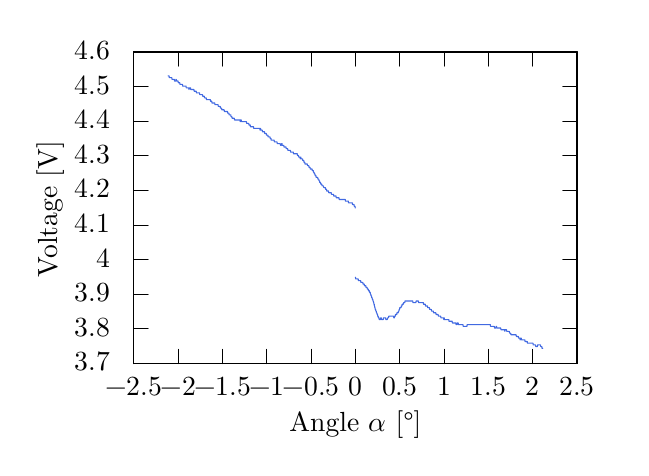
\begin{tikzpicture}[gnuplot]
%% generated with GNUPLOT 5.2p5a (Gentoo revision r0) (Lua 5.1; terminal rev. 99 , script rev. 107)
%% Mi 01 Mai 2019 12:59:13 CEST
\path (0.000,0.000) rectangle (7.500,5.250);
\gpcolor{color=gp lt color border}
\gpsetlinetype{gp lt border}
\gpsetdashtype{gp dt solid}
\gpsetlinewidth{1.00}
\draw[gp path] (1.320,0.985)--(1.500,0.985);
\draw[gp path] (6.947,0.985)--(6.767,0.985);
\node[gp node right] at (1.136,0.985) {$3.7$};
\draw[gp path] (1.320,1.425)--(1.500,1.425);
\draw[gp path] (6.947,1.425)--(6.767,1.425);
\node[gp node right] at (1.136,1.425) {$3.8$};
\draw[gp path] (1.320,1.864)--(1.500,1.864);
\draw[gp path] (6.947,1.864)--(6.767,1.864);
\node[gp node right] at (1.136,1.864) {$3.9$};
\draw[gp path] (1.320,2.304)--(1.500,2.304);
\draw[gp path] (6.947,2.304)--(6.767,2.304);
\node[gp node right] at (1.136,2.304) {$4$};
\draw[gp path] (1.320,2.743)--(1.500,2.743);
\draw[gp path] (6.947,2.743)--(6.767,2.743);
\node[gp node right] at (1.136,2.743) {$4.1$};
\draw[gp path] (1.320,3.183)--(1.500,3.183);
\draw[gp path] (6.947,3.183)--(6.767,3.183);
\node[gp node right] at (1.136,3.183) {$4.2$};
\draw[gp path] (1.320,3.622)--(1.500,3.622);
\draw[gp path] (6.947,3.622)--(6.767,3.622);
\node[gp node right] at (1.136,3.622) {$4.3$};
\draw[gp path] (1.320,4.062)--(1.500,4.062);
\draw[gp path] (6.947,4.062)--(6.767,4.062);
\node[gp node right] at (1.136,4.062) {$4.4$};
\draw[gp path] (1.320,4.501)--(1.500,4.501);
\draw[gp path] (6.947,4.501)--(6.767,4.501);
\node[gp node right] at (1.136,4.501) {$4.5$};
\draw[gp path] (1.320,4.941)--(1.500,4.941);
\draw[gp path] (6.947,4.941)--(6.767,4.941);
\node[gp node right] at (1.136,4.941) {$4.6$};
\draw[gp path] (1.320,0.985)--(1.320,1.165);
\draw[gp path] (1.320,4.941)--(1.320,4.761);
\node[gp node center] at (1.320,0.677) {$-2.5$};
\draw[gp path] (1.883,0.985)--(1.883,1.165);
\draw[gp path] (1.883,4.941)--(1.883,4.761);
\node[gp node center] at (1.883,0.677) {$-2$};
\draw[gp path] (2.445,0.985)--(2.445,1.165);
\draw[gp path] (2.445,4.941)--(2.445,4.761);
\node[gp node center] at (2.445,0.677) {$-1.5$};
\draw[gp path] (3.008,0.985)--(3.008,1.165);
\draw[gp path] (3.008,4.941)--(3.008,4.761);
\node[gp node center] at (3.008,0.677) {$-1$};
\draw[gp path] (3.571,0.985)--(3.571,1.165);
\draw[gp path] (3.571,4.941)--(3.571,4.761);
\node[gp node center] at (3.571,0.677) {$-0.5$};
\draw[gp path] (4.134,0.985)--(4.134,1.165);
\draw[gp path] (4.134,4.941)--(4.134,4.761);
\node[gp node center] at (4.134,0.677) {$0$};
\draw[gp path] (4.696,0.985)--(4.696,1.165);
\draw[gp path] (4.696,4.941)--(4.696,4.761);
\node[gp node center] at (4.696,0.677) {$0.5$};
\draw[gp path] (5.259,0.985)--(5.259,1.165);
\draw[gp path] (5.259,4.941)--(5.259,4.761);
\node[gp node center] at (5.259,0.677) {$1$};
\draw[gp path] (5.822,0.985)--(5.822,1.165);
\draw[gp path] (5.822,4.941)--(5.822,4.761);
\node[gp node center] at (5.822,0.677) {$1.5$};
\draw[gp path] (6.384,0.985)--(6.384,1.165);
\draw[gp path] (6.384,4.941)--(6.384,4.761);
\node[gp node center] at (6.384,0.677) {$2$};
\draw[gp path] (6.947,0.985)--(6.947,1.165);
\draw[gp path] (6.947,4.941)--(6.947,4.761);
\node[gp node center] at (6.947,0.677) {$2.5$};
\draw[gp path] (1.320,4.941)--(1.320,0.985)--(6.947,0.985)--(6.947,4.941)--cycle;
\node[gp node center,rotate=-270] at (0.276,2.963) {Voltage [V]};
\node[gp node center] at (4.133,0.215) {Angle $\alpha$ [°]};
\gpcolor{rgb color={0.255,0.412,0.882}}
\draw[gp path] (4.134,2.961)--(4.131,2.961)--(4.128,2.982)--(4.126,2.982)--(4.123,2.982)%
  --(4.120,2.982)--(4.118,2.982)--(4.115,3.004)--(4.112,3.004)--(4.110,3.004)--(4.107,3.004)%
  --(4.104,3.004)--(4.102,3.004)--(4.099,3.004)--(4.096,3.004)--(4.094,3.025)--(4.091,3.025)%
  --(4.089,3.025)--(4.086,3.025)--(4.083,3.025)--(4.081,3.025)--(4.078,3.025)--(4.075,3.025)%
  --(4.073,3.025)--(4.070,3.025)--(4.067,3.025)--(4.065,3.025)--(4.062,3.025)--(4.059,3.025)%
  --(4.057,3.025)--(4.054,3.025)--(4.051,3.025)--(4.049,3.025)--(4.046,3.025)--(4.044,3.047)%
  --(4.041,3.047)--(4.038,3.047)--(4.036,3.047)--(4.033,3.047)--(4.030,3.047)--(4.028,3.047)%
  --(4.025,3.047)--(4.022,3.047)--(4.020,3.047)--(4.017,3.047)--(4.014,3.047)--(4.012,3.047)%
  --(4.009,3.047)--(4.006,3.047)--(4.004,3.068)--(4.001,3.068)--(3.999,3.068)--(3.996,3.068)%
  --(3.993,3.068)--(3.991,3.068)--(3.988,3.068)--(3.985,3.068)--(3.983,3.068)--(3.980,3.068)%
  --(3.977,3.068)--(3.975,3.068)--(3.972,3.068)--(3.969,3.068)--(3.967,3.068)--(3.964,3.068)%
  --(3.961,3.068)--(3.959,3.068)--(3.956,3.068)--(3.954,3.068)--(3.951,3.068)--(3.948,3.068)%
  --(3.946,3.068)--(3.943,3.068)--(3.940,3.068)--(3.938,3.068)--(3.935,3.068)--(3.932,3.068)%
  --(3.930,3.068)--(3.927,3.068)--(3.924,3.090)--(3.922,3.090)--(3.919,3.090)--(3.916,3.090)%
  --(3.914,3.090)--(3.911,3.090)--(3.909,3.090)--(3.906,3.090)--(3.903,3.090)--(3.901,3.090)%
  --(3.898,3.090)--(3.895,3.090)--(3.893,3.090)--(3.890,3.090)--(3.887,3.112)--(3.885,3.112)%
  --(3.882,3.112)--(3.879,3.112)--(3.877,3.112)--(3.874,3.112)--(3.871,3.112)--(3.869,3.112)%
  --(3.866,3.112)--(3.864,3.112)--(3.861,3.112)--(3.858,3.112)--(3.856,3.133)--(3.853,3.133)%
  --(3.850,3.133)--(3.848,3.133)--(3.845,3.133)--(3.842,3.133)--(3.840,3.133)--(3.837,3.133)%
  --(3.834,3.133)--(3.832,3.133)--(3.829,3.133)--(3.826,3.154)--(3.824,3.154)--(3.821,3.154)%
  --(3.819,3.154)--(3.816,3.154)--(3.813,3.154)--(3.811,3.154)--(3.808,3.154)--(3.805,3.154)%
  --(3.803,3.154)--(3.800,3.154)--(3.797,3.154)--(3.795,3.154)--(3.792,3.176)--(3.789,3.176)%
  --(3.787,3.176)--(3.784,3.176)--(3.781,3.176)--(3.779,3.176)--(3.776,3.176)--(3.774,3.176)%
  --(3.771,3.176)--(3.768,3.176)--(3.766,3.197)--(3.763,3.197)--(3.760,3.197)--(3.758,3.197)%
  --(3.755,3.197)--(3.752,3.219)--(3.750,3.219)--(3.747,3.219)--(3.744,3.219)--(3.742,3.219)%
  --(3.739,3.219)--(3.736,3.219)--(3.734,3.219)--(3.731,3.219)--(3.729,3.240)--(3.726,3.240)%
  --(3.723,3.240)--(3.721,3.240)--(3.718,3.240)--(3.715,3.240)--(3.713,3.240)--(3.710,3.240)%
  --(3.707,3.262)--(3.705,3.262)--(3.702,3.262)--(3.699,3.262)--(3.697,3.262)--(3.694,3.262)%
  --(3.691,3.283)--(3.689,3.283)--(3.686,3.283)--(3.684,3.283)--(3.681,3.283)--(3.678,3.305)%
  --(3.676,3.305)--(3.673,3.305)--(3.670,3.305)--(3.668,3.326)--(3.665,3.326)--(3.662,3.326)%
  --(3.660,3.326)--(3.657,3.326)--(3.654,3.348)--(3.652,3.348)--(3.649,3.348)--(3.646,3.348)%
  --(3.644,3.348)--(3.641,3.348)--(3.639,3.348)--(3.636,3.348)--(3.633,3.369)--(3.631,3.369)%
  --(3.628,3.369)--(3.625,3.369)--(3.623,3.369)--(3.620,3.391)--(3.617,3.391)--(3.615,3.391)%
  --(3.612,3.391)--(3.609,3.412)--(3.607,3.412)--(3.604,3.412)--(3.601,3.412)--(3.599,3.434)%
  --(3.596,3.434)--(3.594,3.434)--(3.591,3.434)--(3.588,3.434)--(3.586,3.434)--(3.583,3.455)%
  --(3.580,3.455)--(3.578,3.455)--(3.575,3.455)--(3.572,3.455)--(3.570,3.455)--(3.567,3.455)%
  --(3.564,3.455)--(3.562,3.455)--(3.559,3.455)--(3.556,3.477)--(3.554,3.477)--(3.551,3.477)%
  --(3.549,3.477)--(3.546,3.477)--(3.543,3.477)--(3.541,3.498)--(3.538,3.498)--(3.535,3.498)%
  --(3.533,3.498)--(3.530,3.498)--(3.527,3.498)--(3.525,3.498)--(3.522,3.519)--(3.519,3.519)%
  --(3.517,3.519)--(3.514,3.519)--(3.511,3.519)--(3.509,3.519)--(3.506,3.519)--(3.504,3.519)%
  --(3.501,3.519)--(3.498,3.519)--(3.496,3.519)--(3.493,3.519)--(3.490,3.541)--(3.488,3.541)%
  --(3.485,3.541)--(3.482,3.541)--(3.480,3.541)--(3.477,3.563)--(3.474,3.563)--(3.472,3.563)%
  --(3.469,3.563)--(3.466,3.563)--(3.464,3.563)--(3.461,3.584)--(3.459,3.584)--(3.456,3.584)%
  --(3.453,3.584)--(3.451,3.584)--(3.448,3.584)--(3.445,3.584)--(3.443,3.584)--(3.440,3.606)%
  --(3.437,3.606)--(3.435,3.606)--(3.432,3.584)--(3.429,3.606)--(3.427,3.606)--(3.424,3.606)%
  --(3.421,3.606)--(3.419,3.606)--(3.416,3.606)--(3.414,3.606)--(3.411,3.627)--(3.408,3.627)%
  --(3.406,3.627)--(3.403,3.627)--(3.400,3.627)--(3.398,3.627)--(3.395,3.649)--(3.392,3.649)%
  --(3.390,3.649)--(3.387,3.649)--(3.384,3.649)--(3.382,3.649)--(3.379,3.649)--(3.376,3.649)%
  --(3.374,3.649)--(3.371,3.649)--(3.369,3.649)--(3.366,3.649)--(3.363,3.649)--(3.361,3.649)%
  --(3.358,3.649)--(3.355,3.649)--(3.353,3.649)--(3.350,3.649)--(3.347,3.649)--(3.345,3.670)%
  --(3.342,3.670)--(3.339,3.670)--(3.337,3.670)--(3.334,3.670)--(3.331,3.670)--(3.329,3.670)%
  --(3.326,3.670)--(3.324,3.670)--(3.321,3.670)--(3.318,3.670)--(3.316,3.670)--(3.313,3.670)%
  --(3.310,3.670)--(3.308,3.691)--(3.305,3.691)--(3.302,3.691)--(3.300,3.691)--(3.297,3.691)%
  --(3.294,3.691)--(3.292,3.691)--(3.289,3.691)--(3.286,3.691)--(3.284,3.691)--(3.281,3.691)%
  --(3.279,3.691)--(3.276,3.691)--(3.273,3.713)--(3.271,3.713)--(3.268,3.713)--(3.265,3.713)%
  --(3.263,3.713)--(3.260,3.713)--(3.257,3.713)--(3.255,3.713)--(3.252,3.734)--(3.249,3.734)%
  --(3.247,3.734)--(3.244,3.734)--(3.241,3.734)--(3.239,3.734)--(3.236,3.734)--(3.234,3.734)%
  --(3.231,3.734)--(3.228,3.734)--(3.226,3.734)--(3.223,3.756)--(3.220,3.756)--(3.218,3.756)%
  --(3.215,3.756)--(3.212,3.756)--(3.210,3.756)--(3.207,3.756)--(3.204,3.756)--(3.202,3.777)%
  --(3.199,3.777)--(3.196,3.777)--(3.194,3.756)--(3.191,3.756)--(3.189,3.756)--(3.186,3.756)%
  --(3.183,3.756)--(3.181,3.756)--(3.178,3.777)--(3.175,3.777)--(3.173,3.777)--(3.170,3.777)%
  --(3.167,3.777)--(3.165,3.777)--(3.162,3.777)--(3.159,3.777)--(3.157,3.777)--(3.154,3.777)%
  --(3.151,3.777)--(3.149,3.777)--(3.146,3.777)--(3.144,3.777)--(3.141,3.777)--(3.138,3.799)%
  --(3.136,3.799)--(3.133,3.799)--(3.130,3.799)--(3.128,3.799)--(3.125,3.799)--(3.122,3.799)%
  --(3.120,3.799)--(3.117,3.799)--(3.114,3.799)--(3.112,3.799)--(3.109,3.799)--(3.106,3.799)%
  --(3.104,3.799)--(3.101,3.821)--(3.099,3.821)--(3.096,3.821)--(3.093,3.821)--(3.091,3.821)%
  --(3.088,3.821)--(3.085,3.821)--(3.083,3.821)--(3.080,3.821)--(3.077,3.821)--(3.075,3.821)%
  --(3.072,3.821)--(3.069,3.821)--(3.067,3.821)--(3.064,3.821)--(3.061,3.842)--(3.059,3.842)%
  --(3.056,3.842)--(3.054,3.842)--(3.051,3.842)--(3.048,3.863)--(3.046,3.863)--(3.043,3.863)%
  --(3.040,3.863)--(3.038,3.863)--(3.035,3.863)--(3.032,3.863)--(3.030,3.863)--(3.027,3.863)%
  --(3.024,3.863)--(3.022,3.885)--(3.019,3.885)--(3.016,3.885)--(3.014,3.885)--(3.011,3.885)%
  --(3.009,3.885)--(3.006,3.885)--(3.003,3.885)--(3.001,3.906)--(2.998,3.906)--(2.995,3.906)%
  --(2.993,3.906)--(2.990,3.906)--(2.987,3.906)--(2.985,3.906)--(2.982,3.906)--(2.979,3.928)%
  --(2.977,3.928)--(2.974,3.928)--(2.971,3.928)--(2.969,3.928)--(2.966,3.928)--(2.964,3.928)%
  --(2.961,3.928)--(2.958,3.928)--(2.956,3.928)--(2.953,3.928)--(2.950,3.949)--(2.948,3.949)%
  --(2.945,3.949)--(2.942,3.949)--(2.940,3.949)--(2.937,3.949)--(2.934,3.949)--(2.932,3.949)%
  --(2.929,3.971)--(2.926,3.949)--(2.924,3.949)--(2.921,3.949)--(2.919,3.971)--(2.916,3.971)%
  --(2.913,3.971)--(2.911,3.971)--(2.908,3.971)--(2.905,3.971)--(2.903,3.971)--(2.900,3.971)%
  --(2.897,3.971)--(2.895,3.971)--(2.892,3.971)--(2.889,3.971)--(2.887,3.971)--(2.884,3.971)%
  --(2.881,3.971)--(2.879,3.971)--(2.876,3.971)--(2.874,3.971)--(2.871,3.971)--(2.868,3.971)%
  --(2.866,3.971)--(2.863,3.971)--(2.860,3.971)--(2.858,3.971)--(2.855,3.971)--(2.852,3.971)%
  --(2.850,3.971)--(2.847,3.971)--(2.844,3.971)--(2.842,3.971)--(2.839,3.992)--(2.836,3.992)%
  --(2.834,3.992)--(2.831,3.992)--(2.829,3.992)--(2.826,3.992)--(2.823,3.992)--(2.821,3.992)%
  --(2.818,3.992)--(2.815,3.992)--(2.813,3.992)--(2.810,3.992)--(2.807,3.992)--(2.805,3.992)%
  --(2.802,3.992)--(2.799,3.992)--(2.797,4.014)--(2.794,4.014)--(2.792,4.014)--(2.789,4.014)%
  --(2.786,4.014)--(2.784,4.014)--(2.781,4.014)--(2.778,4.035)--(2.776,4.035)--(2.773,4.035)%
  --(2.770,4.035)--(2.768,4.035)--(2.765,4.035)--(2.762,4.035)--(2.760,4.035)--(2.757,4.035)%
  --(2.754,4.035)--(2.752,4.035)--(2.749,4.057)--(2.747,4.057)--(2.744,4.057)--(2.741,4.057)%
  --(2.739,4.057)--(2.736,4.057)--(2.733,4.057)--(2.731,4.057)--(2.728,4.057)--(2.725,4.057)%
  --(2.723,4.057)--(2.720,4.057)--(2.717,4.057)--(2.715,4.057)--(2.712,4.057)--(2.709,4.057)%
  --(2.707,4.057)--(2.704,4.057)--(2.702,4.057)--(2.699,4.057)--(2.696,4.057)--(2.694,4.057)%
  --(2.691,4.057)--(2.688,4.057)--(2.686,4.057)--(2.683,4.078)--(2.680,4.078)--(2.678,4.078)%
  --(2.675,4.078)--(2.672,4.057)--(2.670,4.057)--(2.667,4.078)--(2.664,4.078)--(2.662,4.078)%
  --(2.659,4.078)--(2.657,4.078)--(2.654,4.078)--(2.651,4.078)--(2.649,4.078)--(2.646,4.078)%
  --(2.643,4.078)--(2.641,4.078)--(2.638,4.078)--(2.635,4.078)--(2.633,4.078)--(2.630,4.078)%
  --(2.627,4.078)--(2.625,4.078)--(2.622,4.078)--(2.619,4.078)--(2.617,4.078)--(2.614,4.078)%
  --(2.612,4.078)--(2.609,4.078)--(2.606,4.078)--(2.604,4.078)--(2.601,4.078)--(2.598,4.078)%
  --(2.596,4.100)--(2.593,4.100)--(2.590,4.100)--(2.588,4.100)--(2.585,4.100)--(2.582,4.100)%
  --(2.580,4.100)--(2.577,4.100)--(2.574,4.100)--(2.572,4.100)--(2.569,4.100)--(2.567,4.100)%
  --(2.564,4.121)--(2.561,4.121)--(2.559,4.121)--(2.556,4.121)--(2.553,4.121)--(2.551,4.143)%
  --(2.548,4.143)--(2.545,4.143)--(2.543,4.143)--(2.540,4.143)--(2.537,4.143)--(2.535,4.143)%
  --(2.532,4.143)--(2.529,4.143)--(2.527,4.164)--(2.524,4.164)--(2.522,4.164)--(2.519,4.164)%
  --(2.516,4.164)--(2.514,4.164)--(2.511,4.164)--(2.508,4.186)--(2.506,4.186)--(2.503,4.186)%
  --(2.500,4.186)--(2.498,4.186)--(2.495,4.186)--(2.492,4.186)--(2.490,4.186)--(2.487,4.186)%
  --(2.484,4.186)--(2.482,4.186)--(2.479,4.186)--(2.477,4.186)--(2.474,4.186)--(2.471,4.186)%
  --(2.469,4.186)--(2.466,4.207)--(2.463,4.207)--(2.461,4.207)--(2.458,4.207)--(2.455,4.207)%
  --(2.453,4.207)--(2.450,4.207)--(2.447,4.207)--(2.445,4.207)--(2.442,4.207)--(2.439,4.207)%
  --(2.437,4.207)--(2.434,4.228)--(2.432,4.228)--(2.429,4.228)--(2.426,4.228)--(2.424,4.228)%
  --(2.421,4.228)--(2.418,4.228)--(2.416,4.250)--(2.413,4.250)--(2.410,4.250)--(2.408,4.250)%
  --(2.405,4.250)--(2.402,4.250)--(2.400,4.250)--(2.397,4.250)--(2.394,4.250)--(2.392,4.250)%
  --(2.389,4.272)--(2.387,4.272)--(2.384,4.272)--(2.381,4.272)--(2.379,4.272)--(2.376,4.272)%
  --(2.373,4.272)--(2.371,4.272)--(2.368,4.272)--(2.365,4.272)--(2.363,4.272)--(2.360,4.272)%
  --(2.357,4.272)--(2.355,4.272)--(2.352,4.272)--(2.349,4.272)--(2.347,4.293)--(2.344,4.293)%
  --(2.342,4.293)--(2.339,4.293)--(2.336,4.293)--(2.334,4.293)--(2.331,4.293)--(2.328,4.293)%
  --(2.326,4.293)--(2.323,4.293)--(2.320,4.293)--(2.318,4.293)--(2.315,4.293)--(2.312,4.293)%
  --(2.310,4.315)--(2.307,4.315)--(2.304,4.315)--(2.302,4.315)--(2.299,4.315)--(2.297,4.315)%
  --(2.294,4.315)--(2.291,4.336)--(2.289,4.336)--(2.286,4.336)--(2.283,4.336)--(2.281,4.336)%
  --(2.278,4.336)--(2.275,4.336)--(2.273,4.336)--(2.270,4.336)--(2.267,4.336)--(2.265,4.336)%
  --(2.262,4.336)--(2.259,4.336)--(2.257,4.336)--(2.254,4.336)--(2.252,4.336)--(2.249,4.336)%
  --(2.246,4.336)--(2.244,4.336)--(2.241,4.336)--(2.238,4.358)--(2.236,4.358)--(2.233,4.358)%
  --(2.230,4.358)--(2.228,4.358)--(2.225,4.358)--(2.222,4.358)--(2.220,4.358)--(2.217,4.358)%
  --(2.214,4.379)--(2.212,4.379)--(2.209,4.379)--(2.207,4.379)--(2.204,4.379)--(2.201,4.379)%
  --(2.199,4.379)--(2.196,4.379)--(2.193,4.379)--(2.191,4.400)--(2.188,4.400)--(2.185,4.400)%
  --(2.183,4.400)--(2.180,4.400)--(2.177,4.400)--(2.175,4.400)--(2.172,4.400)--(2.169,4.400)%
  --(2.167,4.400)--(2.164,4.400)--(2.162,4.400)--(2.159,4.400)--(2.156,4.400)--(2.154,4.422)%
  --(2.151,4.422)--(2.148,4.422)--(2.146,4.422)--(2.143,4.422)--(2.140,4.422)--(2.138,4.422)%
  --(2.135,4.422)--(2.132,4.422)--(2.130,4.422)--(2.127,4.422)--(2.124,4.422)--(2.122,4.422)%
  --(2.119,4.422)--(2.117,4.422)--(2.114,4.422)--(2.111,4.443)--(2.109,4.443)--(2.106,4.443)%
  --(2.103,4.443)--(2.101,4.443)--(2.098,4.443)--(2.095,4.443)--(2.093,4.443)--(2.090,4.443)%
  --(2.087,4.443)--(2.085,4.443)--(2.082,4.465)--(2.079,4.465)--(2.077,4.465)--(2.074,4.465)%
  --(2.072,4.465)--(2.069,4.465)--(2.066,4.465)--(2.064,4.465)--(2.061,4.465)--(2.058,4.465)%
  --(2.056,4.465)--(2.053,4.465)--(2.050,4.465)--(2.048,4.465)--(2.045,4.465)--(2.042,4.465)%
  --(2.040,4.486)--(2.037,4.486)--(2.034,4.486)--(2.032,4.486)--(2.029,4.486)--(2.027,4.486)%
  --(2.024,4.486)--(2.021,4.465)--(2.019,4.465)--(2.016,4.486)--(2.013,4.486)--(2.011,4.486)%
  --(2.008,4.486)--(2.005,4.486)--(2.003,4.486)--(2.000,4.486)--(1.997,4.486)--(1.995,4.486)%
  --(1.992,4.486)--(1.989,4.486)--(1.987,4.486)--(1.984,4.486)--(1.982,4.508)--(1.979,4.508)%
  --(1.976,4.508)--(1.974,4.508)--(1.971,4.508)--(1.968,4.508)--(1.966,4.508)--(1.963,4.508)%
  --(1.960,4.508)--(1.958,4.508)--(1.955,4.508)--(1.952,4.508)--(1.950,4.508)--(1.947,4.508)%
  --(1.944,4.508)--(1.942,4.508)--(1.939,4.508)--(1.937,4.530)--(1.934,4.530)--(1.931,4.530)%
  --(1.929,4.530)--(1.926,4.530)--(1.923,4.530)--(1.921,4.530)--(1.918,4.530)--(1.915,4.530)%
  --(1.913,4.530)--(1.910,4.530)--(1.907,4.530)--(1.905,4.530)--(1.902,4.551)--(1.899,4.551)%
  --(1.897,4.551)--(1.894,4.551)--(1.892,4.551)--(1.889,4.551)--(1.886,4.551)--(1.884,4.551)%
  --(1.881,4.572)--(1.878,4.572)--(1.876,4.572)--(1.873,4.572)--(1.870,4.572)--(1.868,4.572)%
  --(1.865,4.572)--(1.862,4.572)--(1.860,4.572)--(1.857,4.594)--(1.854,4.594)--(1.852,4.572)%
  --(1.849,4.572)--(1.847,4.572)--(1.844,4.572)--(1.841,4.572)--(1.839,4.572)--(1.836,4.572)%
  --(1.833,4.594)--(1.831,4.594)--(1.828,4.594)--(1.825,4.594)--(1.823,4.594)--(1.820,4.594)%
  --(1.817,4.594)--(1.815,4.594)--(1.812,4.594)--(1.809,4.594)--(1.807,4.594)--(1.804,4.594)%
  --(1.802,4.615)--(1.799,4.615)--(1.796,4.615)--(1.794,4.615)--(1.791,4.615)--(1.788,4.615)%
  --(1.786,4.615)--(1.783,4.615)--(1.780,4.615)--(1.778,4.615)--(1.775,4.615)--(1.772,4.615)%
  --(1.770,4.615)--(1.767,4.637)--(1.764,4.637)--(1.762,4.637)--(1.759,4.637)--(1.757,4.637)%
  --(1.754,4.637);
\draw[gp path] (4.134,2.080)--(4.136,2.059)--(4.139,2.059)--(4.141,2.059)--(4.144,2.059)%
  --(4.147,2.059)--(4.149,2.059)--(4.152,2.059)--(4.155,2.059)--(4.157,2.059)--(4.160,2.059)%
  --(4.163,2.059)--(4.165,2.059)--(4.168,2.059)--(4.171,2.037)--(4.173,2.037)--(4.176,2.037)%
  --(4.178,2.037)--(4.181,2.037)--(4.184,2.037)--(4.186,2.037)--(4.189,2.037)--(4.192,2.037)%
  --(4.194,2.037)--(4.197,2.037)--(4.200,2.037)--(4.202,2.016)--(4.205,2.016)--(4.208,2.016)%
  --(4.210,2.016)--(4.213,2.016)--(4.216,2.016)--(4.218,2.016)--(4.221,2.016)--(4.223,2.016)%
  --(4.226,2.016)--(4.229,1.994)--(4.231,1.994)--(4.234,1.994)--(4.237,1.994)--(4.239,1.994)%
  --(4.242,1.994)--(4.245,1.994)--(4.247,1.973)--(4.250,1.973)--(4.253,1.973)--(4.255,1.973)%
  --(4.258,1.973)--(4.261,1.973)--(4.263,1.973)--(4.266,1.973)--(4.268,1.951)--(4.271,1.951)%
  --(4.274,1.951)--(4.276,1.951)--(4.279,1.951)--(4.282,1.951)--(4.284,1.930)--(4.287,1.930)%
  --(4.290,1.930)--(4.292,1.930)--(4.295,1.930)--(4.298,1.930)--(4.300,1.909)--(4.303,1.909)%
  --(4.306,1.909)--(4.308,1.909)--(4.311,1.909)--(4.313,1.887)--(4.316,1.887)--(4.319,1.887)%
  --(4.321,1.887)--(4.324,1.865)--(4.327,1.865)--(4.329,1.865)--(4.332,1.844)--(4.335,1.844)%
  --(4.337,1.844)--(4.340,1.822)--(4.343,1.822)--(4.345,1.822)--(4.348,1.801)--(4.351,1.801)%
  --(4.353,1.801)--(4.356,1.779)--(4.358,1.779)--(4.361,1.779)--(4.364,1.758)--(4.366,1.758)%
  --(4.369,1.737)--(4.372,1.737)--(4.374,1.715)--(4.377,1.715)--(4.380,1.694)--(4.382,1.694)%
  --(4.385,1.672)--(4.388,1.672)--(4.390,1.672)--(4.393,1.650)--(4.396,1.650)--(4.398,1.650)%
  --(4.401,1.629)--(4.403,1.629)--(4.406,1.629)--(4.409,1.607)--(4.411,1.607)--(4.414,1.607)%
  --(4.417,1.586)--(4.419,1.586)--(4.422,1.586)--(4.425,1.565)--(4.427,1.565)--(4.430,1.565)%
  --(4.433,1.565)--(4.435,1.543)--(4.438,1.543)--(4.441,1.543)--(4.443,1.543)--(4.446,1.543)%
  --(4.448,1.543)--(4.451,1.543)--(4.454,1.565)--(4.456,1.565)--(4.459,1.565)--(4.462,1.565)%
  --(4.464,1.543)--(4.467,1.543)--(4.470,1.543)--(4.472,1.543)--(4.475,1.543)--(4.478,1.543)%
  --(4.480,1.543)--(4.483,1.543)--(4.486,1.543)--(4.488,1.565)--(4.491,1.565)--(4.493,1.565)%
  --(4.496,1.565)--(4.499,1.565)--(4.501,1.565)--(4.504,1.565)--(4.507,1.565)--(4.509,1.565)%
  --(4.512,1.565)--(4.515,1.565)--(4.517,1.565)--(4.520,1.543)--(4.523,1.543)--(4.525,1.543)%
  --(4.528,1.543)--(4.531,1.543)--(4.533,1.543)--(4.536,1.543)--(4.538,1.543)--(4.541,1.565)%
  --(4.544,1.565)--(4.546,1.565)--(4.549,1.565)--(4.552,1.565)--(4.554,1.565)--(4.557,1.586)%
  --(4.560,1.586)--(4.562,1.586)--(4.565,1.586)--(4.568,1.586)--(4.570,1.586)--(4.573,1.586)%
  --(4.576,1.586)--(4.578,1.586)--(4.581,1.586)--(4.583,1.586)--(4.586,1.586)--(4.589,1.586)%
  --(4.591,1.586)--(4.594,1.586)--(4.597,1.586)--(4.599,1.586)--(4.602,1.586)--(4.605,1.586)%
  --(4.607,1.586)--(4.610,1.586)--(4.613,1.586)--(4.615,1.586)--(4.618,1.586)--(4.621,1.565)%
  --(4.623,1.565)--(4.626,1.565)--(4.628,1.565)--(4.631,1.586)--(4.634,1.586)--(4.636,1.586)%
  --(4.639,1.586)--(4.642,1.607)--(4.644,1.607)--(4.647,1.607)--(4.650,1.607)--(4.652,1.607)%
  --(4.655,1.607)--(4.658,1.607)--(4.660,1.629)--(4.663,1.629)--(4.666,1.629)--(4.668,1.629)%
  --(4.671,1.629)--(4.673,1.629)--(4.676,1.629)--(4.679,1.650)--(4.681,1.650)--(4.684,1.650)%
  --(4.687,1.650)--(4.689,1.672)--(4.692,1.672)--(4.695,1.672)--(4.697,1.694)--(4.700,1.694)%
  --(4.703,1.694)--(4.705,1.694)--(4.708,1.694)--(4.711,1.694)--(4.713,1.694)--(4.716,1.715)%
  --(4.718,1.715)--(4.721,1.715)--(4.724,1.715)--(4.726,1.737)--(4.729,1.737)--(4.732,1.737)%
  --(4.734,1.737)--(4.737,1.737)--(4.740,1.737)--(4.742,1.737)--(4.745,1.758)--(4.748,1.758)%
  --(4.750,1.758)--(4.753,1.758)--(4.756,1.758)--(4.758,1.758)--(4.761,1.758)--(4.763,1.779)%
  --(4.766,1.779)--(4.769,1.779)--(4.771,1.779)--(4.774,1.779)--(4.777,1.779)--(4.779,1.779)%
  --(4.782,1.779)--(4.785,1.779)--(4.787,1.779)--(4.790,1.779)--(4.793,1.779)--(4.795,1.779)%
  --(4.798,1.779)--(4.801,1.779)--(4.803,1.779)--(4.806,1.779)--(4.808,1.779)--(4.811,1.779)%
  --(4.814,1.779)--(4.816,1.779)--(4.819,1.779)--(4.822,1.779)--(4.824,1.779)--(4.827,1.779)%
  --(4.830,1.779)--(4.832,1.779)--(4.835,1.779)--(4.838,1.779)--(4.840,1.779)--(4.843,1.779)%
  --(4.846,1.779)--(4.848,1.779)--(4.851,1.779)--(4.853,1.779)--(4.856,1.779)--(4.859,1.779)%
  --(4.861,1.779)--(4.864,1.758)--(4.867,1.758)--(4.869,1.758)--(4.872,1.758)--(4.875,1.758)%
  --(4.877,1.758)--(4.880,1.758)--(4.883,1.758)--(4.885,1.758)--(4.888,1.758)--(4.891,1.758)%
  --(4.893,1.758)--(4.896,1.758)--(4.898,1.758)--(4.901,1.758)--(4.904,1.779)--(4.906,1.779)%
  --(4.909,1.779)--(4.912,1.779)--(4.914,1.779)--(4.917,1.779)--(4.920,1.779)--(4.922,1.779)%
  --(4.925,1.779)--(4.928,1.779)--(4.930,1.779)--(4.933,1.779)--(4.936,1.758)--(4.938,1.758)%
  --(4.941,1.758)--(4.943,1.758)--(4.946,1.758)--(4.949,1.758)--(4.951,1.758)--(4.954,1.758)%
  --(4.957,1.758)--(4.959,1.758)--(4.962,1.758)--(4.965,1.758)--(4.967,1.758)--(4.970,1.758)%
  --(4.973,1.758)--(4.975,1.758)--(4.978,1.758)--(4.981,1.758)--(4.983,1.758)--(4.986,1.758)%
  --(4.988,1.758)--(4.991,1.758)--(4.994,1.758)--(4.996,1.758)--(4.999,1.737)--(5.002,1.737)%
  --(5.004,1.737)--(5.007,1.737)--(5.010,1.737)--(5.012,1.737)--(5.015,1.737)--(5.018,1.737)%
  --(5.020,1.737)--(5.023,1.715)--(5.026,1.715)--(5.028,1.715)--(5.031,1.715)--(5.033,1.715)%
  --(5.036,1.715)--(5.039,1.715)--(5.041,1.715)--(5.044,1.715)--(5.047,1.715)--(5.049,1.715)%
  --(5.052,1.694)--(5.055,1.694)--(5.057,1.694)--(5.060,1.694)--(5.063,1.694)--(5.065,1.694)%
  --(5.068,1.694)--(5.071,1.694)--(5.073,1.694)--(5.076,1.672)--(5.078,1.672)--(5.081,1.672)%
  --(5.084,1.672)--(5.086,1.672)--(5.089,1.672)--(5.092,1.672)--(5.094,1.672)--(5.097,1.672)%
  --(5.100,1.650)--(5.102,1.650)--(5.105,1.650)--(5.108,1.650)--(5.110,1.650)--(5.113,1.650)%
  --(5.116,1.650)--(5.118,1.650)--(5.121,1.650)--(5.123,1.650)--(5.126,1.629)--(5.129,1.629)%
  --(5.131,1.629)--(5.134,1.629)--(5.137,1.629)--(5.139,1.629)--(5.142,1.629)--(5.145,1.629)%
  --(5.147,1.629)--(5.150,1.629)--(5.153,1.629)--(5.155,1.629)--(5.158,1.607)--(5.161,1.607)%
  --(5.163,1.607)--(5.166,1.607)--(5.168,1.607)--(5.171,1.607)--(5.174,1.607)--(5.176,1.607)%
  --(5.179,1.607)--(5.182,1.607)--(5.184,1.607)--(5.187,1.586)--(5.190,1.586)--(5.192,1.586)%
  --(5.195,1.586)--(5.198,1.586)--(5.200,1.586)--(5.203,1.586)--(5.206,1.586)--(5.208,1.586)%
  --(5.211,1.586)--(5.213,1.586)--(5.216,1.586)--(5.219,1.565)--(5.221,1.565)--(5.224,1.565)%
  --(5.227,1.565)--(5.229,1.565)--(5.232,1.565)--(5.235,1.565)--(5.237,1.565)--(5.240,1.565)%
  --(5.243,1.565)--(5.245,1.565)--(5.248,1.565)--(5.251,1.565)--(5.253,1.565)--(5.256,1.543)%
  --(5.258,1.543)--(5.261,1.565)--(5.264,1.543)--(5.266,1.543)--(5.269,1.543)--(5.272,1.543)%
  --(5.274,1.543)--(5.277,1.543)--(5.280,1.543)--(5.282,1.543)--(5.285,1.543)--(5.288,1.543)%
  --(5.290,1.543)--(5.293,1.543)--(5.296,1.543)--(5.298,1.543)--(5.301,1.543)--(5.303,1.543)%
  --(5.306,1.543)--(5.309,1.543)--(5.311,1.543)--(5.314,1.543)--(5.317,1.543)--(5.319,1.543)%
  --(5.322,1.522)--(5.325,1.522)--(5.327,1.522)--(5.330,1.522)--(5.333,1.522)--(5.335,1.522)%
  --(5.338,1.522)--(5.341,1.522)--(5.343,1.522)--(5.346,1.522)--(5.348,1.522)--(5.351,1.522)%
  --(5.354,1.522)--(5.356,1.522)--(5.359,1.522)--(5.362,1.522)--(5.364,1.500)--(5.367,1.500)%
  --(5.370,1.500)--(5.372,1.500)--(5.375,1.500)--(5.378,1.500)--(5.380,1.500)--(5.383,1.500)%
  --(5.386,1.500)--(5.388,1.500)--(5.391,1.500)--(5.393,1.500)--(5.396,1.500)--(5.399,1.500)%
  --(5.401,1.500)--(5.404,1.500)--(5.407,1.500)--(5.409,1.500)--(5.412,1.479)--(5.415,1.479)%
  --(5.417,1.479)--(5.420,1.479)--(5.423,1.479)--(5.425,1.500)--(5.428,1.500)--(5.431,1.500)%
  --(5.433,1.500)--(5.436,1.500)--(5.438,1.500)--(5.441,1.479)--(5.444,1.479)--(5.446,1.479)%
  --(5.449,1.479)--(5.452,1.479)--(5.454,1.479)--(5.457,1.479)--(5.460,1.479)--(5.462,1.479)%
  --(5.465,1.479)--(5.468,1.479)--(5.470,1.479)--(5.473,1.479)--(5.475,1.479)--(5.478,1.479)%
  --(5.481,1.479)--(5.483,1.479)--(5.486,1.479)--(5.489,1.479)--(5.491,1.479)--(5.494,1.479)%
  --(5.497,1.479)--(5.499,1.479)--(5.502,1.457)--(5.505,1.457)--(5.507,1.457)--(5.510,1.457)%
  --(5.513,1.457)--(5.515,1.457)--(5.518,1.457)--(5.520,1.457)--(5.523,1.457)--(5.526,1.457)%
  --(5.528,1.457)--(5.531,1.457)--(5.534,1.457)--(5.536,1.457)--(5.539,1.457)--(5.542,1.457)%
  --(5.544,1.457)--(5.547,1.457)--(5.550,1.457)--(5.552,1.479)--(5.555,1.479)--(5.558,1.479)%
  --(5.560,1.479)--(5.563,1.479)--(5.565,1.479)--(5.568,1.479)--(5.571,1.479)--(5.573,1.479)%
  --(5.576,1.479)--(5.579,1.479)--(5.581,1.479)--(5.584,1.479)--(5.587,1.479)--(5.589,1.479)%
  --(5.592,1.479)--(5.595,1.479)--(5.597,1.479)--(5.600,1.479)--(5.603,1.479)--(5.605,1.479)%
  --(5.608,1.479)--(5.610,1.479)--(5.613,1.479)--(5.616,1.479)--(5.618,1.479)--(5.621,1.479)%
  --(5.624,1.479)--(5.626,1.479)--(5.629,1.479)--(5.632,1.479)--(5.634,1.479)--(5.637,1.479)%
  --(5.640,1.479)--(5.642,1.479)--(5.645,1.479)--(5.648,1.479)--(5.650,1.479)--(5.653,1.479)%
  --(5.655,1.479)--(5.658,1.479)--(5.661,1.479)--(5.663,1.479)--(5.666,1.479)--(5.669,1.479)%
  --(5.671,1.479)--(5.674,1.479)--(5.677,1.479)--(5.679,1.479)--(5.682,1.479)--(5.685,1.479)%
  --(5.687,1.479)--(5.690,1.479)--(5.693,1.479)--(5.695,1.479)--(5.698,1.479)--(5.700,1.479)%
  --(5.703,1.479)--(5.706,1.479)--(5.708,1.479)--(5.711,1.479)--(5.714,1.479)--(5.716,1.479)%
  --(5.719,1.479)--(5.722,1.479)--(5.724,1.479)--(5.727,1.479)--(5.730,1.479)--(5.732,1.479)%
  --(5.735,1.479)--(5.738,1.479)--(5.740,1.479)--(5.743,1.479)--(5.745,1.479)--(5.748,1.479)%
  --(5.751,1.479)--(5.753,1.479)--(5.756,1.479)--(5.759,1.479)--(5.761,1.479)--(5.764,1.479)%
  --(5.767,1.479)--(5.769,1.479)--(5.772,1.479)--(5.775,1.479)--(5.777,1.479)--(5.780,1.479)%
  --(5.783,1.479)--(5.785,1.479)--(5.788,1.479)--(5.790,1.479)--(5.793,1.479)--(5.796,1.479)%
  --(5.798,1.479)--(5.801,1.479)--(5.804,1.479)--(5.806,1.479)--(5.809,1.479)--(5.812,1.479)%
  --(5.814,1.479)--(5.817,1.479)--(5.820,1.479)--(5.822,1.479)--(5.825,1.479)--(5.828,1.479)%
  --(5.830,1.479)--(5.833,1.479)--(5.835,1.479)--(5.838,1.479)--(5.841,1.479)--(5.843,1.479)%
  --(5.846,1.479)--(5.849,1.457)--(5.851,1.457)--(5.854,1.457)--(5.857,1.457)--(5.859,1.457)%
  --(5.862,1.457)--(5.865,1.457)--(5.867,1.457)--(5.870,1.457)--(5.873,1.457)--(5.875,1.457)%
  --(5.878,1.457)--(5.880,1.457)--(5.883,1.457)--(5.886,1.457)--(5.888,1.457)--(5.891,1.457)%
  --(5.894,1.457)--(5.896,1.457)--(5.899,1.436)--(5.902,1.436)--(5.904,1.436)--(5.907,1.436)%
  --(5.910,1.436)--(5.912,1.436)--(5.915,1.436)--(5.918,1.436)--(5.920,1.457)--(5.923,1.457)%
  --(5.925,1.457)--(5.928,1.436)--(5.931,1.436)--(5.933,1.436)--(5.936,1.436)--(5.939,1.436)%
  --(5.941,1.436)--(5.944,1.436)--(5.947,1.436)--(5.949,1.436)--(5.952,1.436)--(5.955,1.436)%
  --(5.957,1.436)--(5.960,1.436)--(5.963,1.436)--(5.965,1.436)--(5.968,1.436)--(5.970,1.436)%
  --(5.973,1.436)--(5.976,1.436)--(5.978,1.436)--(5.981,1.414)--(5.984,1.414)--(5.986,1.414)%
  --(5.989,1.414)--(5.992,1.414)--(5.994,1.414)--(5.997,1.414)--(6.000,1.414)--(6.002,1.414)%
  --(6.005,1.414)--(6.008,1.414)--(6.010,1.414)--(6.013,1.414)--(6.015,1.414)--(6.018,1.414)%
  --(6.021,1.414)--(6.023,1.414)--(6.026,1.414)--(6.029,1.414)--(6.031,1.393)--(6.034,1.414)%
  --(6.037,1.414)--(6.039,1.414)--(6.042,1.414)--(6.045,1.414)--(6.047,1.414)--(6.050,1.414)%
  --(6.053,1.414)--(6.055,1.393)--(6.058,1.393)--(6.060,1.393)--(6.063,1.393)--(6.066,1.393)%
  --(6.068,1.393)--(6.071,1.393)--(6.074,1.393)--(6.076,1.393)--(6.079,1.393)--(6.082,1.393)%
  --(6.084,1.393)--(6.087,1.393)--(6.090,1.371)--(6.092,1.371)--(6.095,1.371)--(6.098,1.371)%
  --(6.100,1.371)--(6.103,1.371)--(6.105,1.371)--(6.108,1.350)--(6.111,1.350)--(6.113,1.350)%
  --(6.116,1.350)--(6.119,1.350)--(6.121,1.350)--(6.124,1.350)--(6.127,1.350)--(6.129,1.350)%
  --(6.132,1.350)--(6.135,1.350)--(6.137,1.350)--(6.140,1.350)--(6.143,1.350)--(6.145,1.350)%
  --(6.148,1.350)--(6.150,1.350)--(6.153,1.350)--(6.156,1.350)--(6.158,1.350)--(6.161,1.350)%
  --(6.164,1.350)--(6.166,1.350)--(6.169,1.350)--(6.172,1.350)--(6.174,1.350)--(6.177,1.328)%
  --(6.180,1.328)--(6.182,1.328)--(6.185,1.328)--(6.188,1.328)--(6.190,1.328)--(6.193,1.328)%
  --(6.195,1.328)--(6.198,1.328)--(6.201,1.328)--(6.203,1.328)--(6.206,1.307)--(6.209,1.307)%
  --(6.211,1.307)--(6.214,1.307)--(6.217,1.307)--(6.219,1.307)--(6.222,1.307)--(6.225,1.285)%
  --(6.227,1.285)--(6.230,1.307)--(6.233,1.307)--(6.235,1.307)--(6.238,1.307)--(6.240,1.307)%
  --(6.243,1.285)--(6.246,1.285)--(6.248,1.285)--(6.251,1.285)--(6.254,1.285)--(6.256,1.285)%
  --(6.259,1.285)--(6.262,1.285)--(6.264,1.285)--(6.267,1.285)--(6.270,1.285)--(6.272,1.285)%
  --(6.275,1.285)--(6.278,1.285)--(6.280,1.285)--(6.283,1.285)--(6.285,1.285)--(6.288,1.264)%
  --(6.291,1.264)--(6.293,1.264)--(6.296,1.264)--(6.299,1.264)--(6.301,1.264)--(6.304,1.264)%
  --(6.307,1.264)--(6.309,1.264)--(6.312,1.264)--(6.315,1.264)--(6.317,1.243)--(6.320,1.243)%
  --(6.323,1.243)--(6.325,1.243)--(6.328,1.243)--(6.330,1.243)--(6.333,1.243)--(6.336,1.243)%
  --(6.338,1.243)--(6.341,1.243)--(6.344,1.243)--(6.346,1.243)--(6.349,1.243)--(6.352,1.243)%
  --(6.354,1.243)--(6.357,1.243)--(6.360,1.243)--(6.362,1.243)--(6.365,1.243)--(6.368,1.243)%
  --(6.370,1.243)--(6.373,1.243)--(6.375,1.243)--(6.378,1.243)--(6.381,1.243)--(6.383,1.243)%
  --(6.386,1.243)--(6.389,1.243)--(6.391,1.221)--(6.394,1.221)--(6.397,1.221)--(6.399,1.221)%
  --(6.402,1.221)--(6.405,1.221)--(6.407,1.221)--(6.410,1.221)--(6.413,1.221)--(6.415,1.221)%
  --(6.418,1.221)--(6.420,1.221)--(6.423,1.200)--(6.426,1.200)--(6.428,1.200)--(6.431,1.200)%
  --(6.434,1.200)--(6.436,1.200)--(6.439,1.200)--(6.442,1.200)--(6.444,1.200)--(6.447,1.221)%
  --(6.450,1.221)--(6.452,1.221)--(6.455,1.221)--(6.458,1.221)--(6.460,1.221)--(6.463,1.221)%
  --(6.465,1.221)--(6.468,1.221)--(6.471,1.221)--(6.473,1.221)--(6.476,1.221)--(6.479,1.221)%
  --(6.481,1.221)--(6.484,1.221)--(6.487,1.200)--(6.489,1.200)--(6.492,1.200)--(6.495,1.200)%
  --(6.497,1.200)--(6.500,1.200)--(6.503,1.178)--(6.505,1.178)--(6.508,1.178)--(6.510,1.178)%
  --(6.513,1.178);
\gpcolor{color=gp lt color border}
\draw[gp path] (1.320,4.941)--(1.320,0.985)--(6.947,0.985)--(6.947,4.941)--cycle;
%% coordinates of the plot area
\gpdefrectangularnode{gp plot 1}{\pgfpoint{1.320cm}{0.985cm}}{\pgfpoint{6.947cm}{4.941cm}}
\end{tikzpicture}
%% gnuplot variables

		\caption{Laser wavenlength 850 nm}
	\end{subfigure}
	\begin{subfigure}{.48\textwidth}
		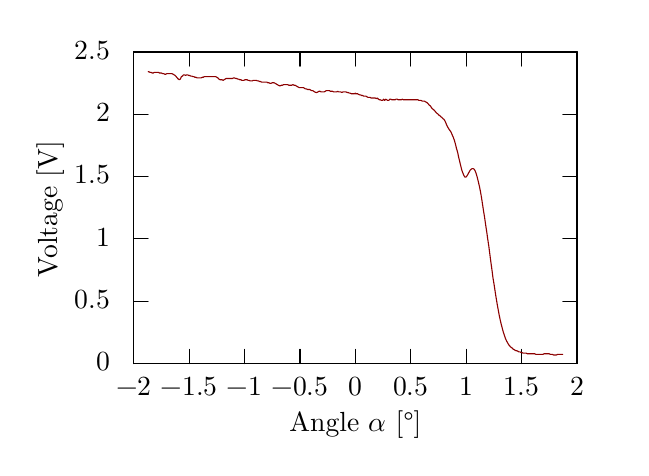
\begin{tikzpicture}[gnuplot]
%% generated with GNUPLOT 5.2p5a (Gentoo revision r0) (Lua 5.1; terminal rev. 99 , script rev. 107)
%% Mi 01 Mai 2019 12:59:13 CEST
\path (0.000,0.000) rectangle (7.500,5.250);
\gpcolor{color=gp lt color border}
\gpsetlinetype{gp lt border}
\gpsetdashtype{gp dt solid}
\gpsetlinewidth{1.00}
\draw[gp path] (1.320,0.985)--(1.500,0.985);
\draw[gp path] (6.947,0.985)--(6.767,0.985);
\node[gp node right] at (1.136,0.985) {$0$};
\draw[gp path] (1.320,1.776)--(1.500,1.776);
\draw[gp path] (6.947,1.776)--(6.767,1.776);
\node[gp node right] at (1.136,1.776) {$0.5$};
\draw[gp path] (1.320,2.567)--(1.500,2.567);
\draw[gp path] (6.947,2.567)--(6.767,2.567);
\node[gp node right] at (1.136,2.567) {$1$};
\draw[gp path] (1.320,3.359)--(1.500,3.359);
\draw[gp path] (6.947,3.359)--(6.767,3.359);
\node[gp node right] at (1.136,3.359) {$1.5$};
\draw[gp path] (1.320,4.150)--(1.500,4.150);
\draw[gp path] (6.947,4.150)--(6.767,4.150);
\node[gp node right] at (1.136,4.150) {$2$};
\draw[gp path] (1.320,4.941)--(1.500,4.941);
\draw[gp path] (6.947,4.941)--(6.767,4.941);
\node[gp node right] at (1.136,4.941) {$2.5$};
\draw[gp path] (1.320,0.985)--(1.320,1.165);
\draw[gp path] (1.320,4.941)--(1.320,4.761);
\node[gp node center] at (1.320,0.677) {$-2$};
\draw[gp path] (2.023,0.985)--(2.023,1.165);
\draw[gp path] (2.023,4.941)--(2.023,4.761);
\node[gp node center] at (2.023,0.677) {$-1.5$};
\draw[gp path] (2.727,0.985)--(2.727,1.165);
\draw[gp path] (2.727,4.941)--(2.727,4.761);
\node[gp node center] at (2.727,0.677) {$-1$};
\draw[gp path] (3.430,0.985)--(3.430,1.165);
\draw[gp path] (3.430,4.941)--(3.430,4.761);
\node[gp node center] at (3.430,0.677) {$-0.5$};
\draw[gp path] (4.134,0.985)--(4.134,1.165);
\draw[gp path] (4.134,4.941)--(4.134,4.761);
\node[gp node center] at (4.134,0.677) {$0$};
\draw[gp path] (4.837,0.985)--(4.837,1.165);
\draw[gp path] (4.837,4.941)--(4.837,4.761);
\node[gp node center] at (4.837,0.677) {$0.5$};
\draw[gp path] (5.540,0.985)--(5.540,1.165);
\draw[gp path] (5.540,4.941)--(5.540,4.761);
\node[gp node center] at (5.540,0.677) {$1$};
\draw[gp path] (6.244,0.985)--(6.244,1.165);
\draw[gp path] (6.244,4.941)--(6.244,4.761);
\node[gp node center] at (6.244,0.677) {$1.5$};
\draw[gp path] (6.947,0.985)--(6.947,1.165);
\draw[gp path] (6.947,4.941)--(6.947,4.761);
\node[gp node center] at (6.947,0.677) {$2$};
\draw[gp path] (1.320,4.941)--(1.320,0.985)--(6.947,0.985)--(6.947,4.941)--cycle;
\node[gp node center,rotate=-270] at (0.276,2.963) {Voltage [V]};
\node[gp node center] at (4.133,0.215) {Angle $\alpha$ [°]};
\gpcolor{rgb color={0.545,0.000,0.000}}
\draw[gp path] (4.134,4.411)--(4.147,4.411)--(4.160,4.411)--(4.173,4.403)--(4.186,4.396)%
  --(4.200,4.396)--(4.213,4.388)--(4.226,4.388)--(4.239,4.380)--(4.253,4.380)--(4.266,4.380)%
  --(4.279,4.373)--(4.292,4.365)--(4.306,4.365)--(4.319,4.365)--(4.332,4.357)--(4.345,4.357)%
  --(4.358,4.357)--(4.372,4.357)--(4.385,4.357)--(4.398,4.349)--(4.411,4.357)--(4.425,4.342)%
  --(4.438,4.334)--(4.451,4.334)--(4.464,4.326)--(4.478,4.326)--(4.491,4.342)--(4.504,4.326)%
  --(4.517,4.342)--(4.531,4.334)--(4.544,4.326)--(4.557,4.326)--(4.570,4.342)--(4.583,4.342)%
  --(4.597,4.334)--(4.610,4.334)--(4.623,4.334)--(4.636,4.334)--(4.650,4.342)--(4.663,4.342)%
  --(4.676,4.334)--(4.689,4.334)--(4.703,4.334)--(4.716,4.334)--(4.729,4.342)--(4.742,4.334)%
  --(4.756,4.334)--(4.769,4.334)--(4.782,4.334)--(4.795,4.334)--(4.808,4.334)--(4.822,4.334)%
  --(4.835,4.334)--(4.848,4.334)--(4.861,4.334)--(4.875,4.334)--(4.888,4.334)--(4.901,4.334)%
  --(4.914,4.334)--(4.928,4.334)--(4.941,4.326)--(4.954,4.326)--(4.967,4.326)--(4.981,4.318)%
  --(4.994,4.318)--(5.007,4.318)--(5.020,4.311)--(5.033,4.303)--(5.047,4.295)--(5.060,4.280)%
  --(5.073,4.264)--(5.086,4.256)--(5.100,4.233)--(5.113,4.218)--(5.126,4.210)--(5.139,4.195)%
  --(5.153,4.179)--(5.166,4.164)--(5.179,4.156)--(5.192,4.140)--(5.206,4.133)--(5.219,4.117)%
  --(5.232,4.110)--(5.245,4.094)--(5.258,4.086)--(5.272,4.063)--(5.285,4.032)--(5.298,4.001)%
  --(5.311,3.978)--(5.325,3.955)--(5.338,3.939)--(5.351,3.916)--(5.364,3.885)--(5.378,3.854)%
  --(5.391,3.816)--(5.404,3.769)--(5.417,3.715)--(5.431,3.669)--(5.444,3.607)--(5.457,3.553)%
  --(5.470,3.499)--(5.483,3.445)--(5.497,3.406)--(5.510,3.375)--(5.523,3.352)--(5.536,3.352)%
  --(5.550,3.367)--(5.563,3.390)--(5.576,3.414)--(5.589,3.437)--(5.603,3.452)--(5.616,3.460)%
  --(5.629,3.460)--(5.642,3.452)--(5.655,3.429)--(5.669,3.390)--(5.682,3.344)--(5.695,3.290)%
  --(5.708,3.236)--(5.722,3.166)--(5.735,3.089)--(5.748,3.004)--(5.761,2.919)--(5.775,2.833)%
  --(5.788,2.741)--(5.801,2.656)--(5.814,2.563)--(5.828,2.470)--(5.841,2.369)--(5.854,2.269)%
  --(5.867,2.176)--(5.880,2.075)--(5.894,1.990)--(5.907,1.905)--(5.920,1.820)--(5.933,1.743)%
  --(5.947,1.666)--(5.960,1.596)--(5.973,1.534)--(5.986,1.480)--(6.000,1.426)--(6.013,1.379)%
  --(6.026,1.341)--(6.039,1.302)--(6.053,1.271)--(6.066,1.248)--(6.079,1.225)--(6.092,1.209)%
  --(6.105,1.194)--(6.119,1.186)--(6.132,1.171)--(6.145,1.163)--(6.158,1.155)--(6.172,1.147)%
  --(6.185,1.147)--(6.198,1.140)--(6.211,1.132)--(6.225,1.132)--(6.238,1.124)--(6.251,1.124)%
  --(6.264,1.116)--(6.278,1.116)--(6.291,1.116)--(6.304,1.116)--(6.317,1.109)--(6.330,1.109)%
  --(6.344,1.109)--(6.357,1.109)--(6.370,1.109)--(6.383,1.109)--(6.397,1.109)--(6.410,1.109)%
  --(6.423,1.101)--(6.436,1.101)--(6.450,1.101)--(6.463,1.101)--(6.476,1.101)--(6.489,1.101)%
  --(6.503,1.101)--(6.516,1.101)--(6.529,1.109)--(6.542,1.109)--(6.555,1.109)--(6.569,1.109)%
  --(6.582,1.109)--(6.595,1.109)--(6.608,1.101)--(6.622,1.101)--(6.635,1.101)--(6.648,1.093)%
  --(6.661,1.093)--(6.675,1.093)--(6.688,1.093)--(6.701,1.101)--(6.714,1.101)--(6.728,1.101)%
  --(6.741,1.101)--(6.754,1.101)--(6.767,1.101);
\draw[gp path] (4.134,4.419)--(4.120,4.411)--(4.107,4.411)--(4.094,4.411)--(4.081,4.411)%
  --(4.067,4.419)--(4.054,4.419)--(4.041,4.427)--(4.028,4.427)--(4.014,4.434)--(4.001,4.434)%
  --(3.988,4.434)--(3.975,4.434)--(3.961,4.427)--(3.948,4.434)--(3.935,4.434)--(3.922,4.434)%
  --(3.909,4.442)--(3.895,4.434)--(3.882,4.434)--(3.869,4.434)--(3.856,4.434)--(3.842,4.442)%
  --(3.829,4.442)--(3.816,4.442)--(3.803,4.450)--(3.789,4.450)--(3.776,4.450)--(3.763,4.450)%
  --(3.750,4.442)--(3.736,4.434)--(3.723,4.434)--(3.710,4.434)--(3.697,4.434)--(3.684,4.442)%
  --(3.670,4.442)--(3.657,4.434)--(3.644,4.427)--(3.631,4.427)--(3.617,4.434)--(3.604,4.442)%
  --(3.591,4.450)--(3.578,4.450)--(3.564,4.458)--(3.551,4.465)--(3.538,4.465)--(3.525,4.465)%
  --(3.511,4.473)--(3.498,4.473)--(3.485,4.481)--(3.472,4.489)--(3.459,4.489)--(3.445,4.489)%
  --(3.432,4.489)--(3.419,4.489)--(3.406,4.496)--(3.392,4.504)--(3.379,4.512)--(3.366,4.519)%
  --(3.353,4.519)--(3.339,4.527)--(3.326,4.519)--(3.313,4.519)--(3.300,4.519)--(3.286,4.519)%
  --(3.273,4.527)--(3.260,4.527)--(3.247,4.527)--(3.234,4.527)--(3.220,4.527)--(3.207,4.519)%
  --(3.194,4.519)--(3.181,4.512)--(3.167,4.512)--(3.154,4.519)--(3.141,4.527)--(3.128,4.535)%
  --(3.114,4.543)--(3.101,4.550)--(3.088,4.550)--(3.075,4.550)--(3.061,4.543)--(3.048,4.543)%
  --(3.035,4.550)--(3.022,4.550)--(3.009,4.558)--(2.995,4.558)--(2.982,4.558)--(2.969,4.558)%
  --(2.956,4.558)--(2.942,4.558)--(2.929,4.566)--(2.916,4.566)--(2.903,4.574)--(2.889,4.574)%
  --(2.876,4.581)--(2.863,4.581)--(2.850,4.581)--(2.836,4.581)--(2.823,4.574)--(2.810,4.574)%
  --(2.797,4.574)--(2.784,4.581)--(2.770,4.581)--(2.757,4.589)--(2.744,4.589)--(2.731,4.589)%
  --(2.717,4.581)--(2.704,4.581)--(2.691,4.581)--(2.678,4.589)--(2.664,4.589)--(2.651,4.597)%
  --(2.638,4.597)--(2.625,4.605)--(2.612,4.605)--(2.598,4.612)--(2.585,4.612)--(2.572,4.605)%
  --(2.559,4.605)--(2.545,4.605)--(2.532,4.605)--(2.519,4.605)--(2.506,4.605)--(2.492,4.605)%
  --(2.479,4.597)--(2.466,4.589)--(2.453,4.581)--(2.439,4.589)--(2.426,4.589)--(2.413,4.589)%
  --(2.400,4.597)--(2.387,4.612)--(2.373,4.620)--(2.360,4.628)--(2.347,4.628)--(2.334,4.628)%
  --(2.320,4.628)--(2.307,4.628)--(2.294,4.628)--(2.281,4.628)--(2.267,4.628)--(2.254,4.628)%
  --(2.241,4.628)--(2.228,4.628)--(2.214,4.628)--(2.201,4.620)--(2.188,4.620)--(2.175,4.612)%
  --(2.162,4.612)--(2.148,4.612)--(2.135,4.612)--(2.122,4.612)--(2.109,4.620)--(2.095,4.620)%
  --(2.082,4.628)--(2.069,4.628)--(2.056,4.635)--(2.042,4.635)--(2.029,4.643)--(2.016,4.643)%
  --(2.003,4.651)--(1.989,4.651)--(1.976,4.643)--(1.963,4.651)--(1.950,4.651)--(1.937,4.635)%
  --(1.923,4.628)--(1.910,4.597)--(1.897,4.589)--(1.884,4.597)--(1.870,4.612)--(1.857,4.628)%
  --(1.844,4.643)--(1.831,4.651)--(1.817,4.659)--(1.804,4.666)--(1.791,4.666)--(1.778,4.666)%
  --(1.764,4.666)--(1.751,4.666)--(1.738,4.666)--(1.725,4.659)--(1.712,4.659)--(1.698,4.666)%
  --(1.685,4.666)--(1.672,4.674)--(1.659,4.674)--(1.645,4.674)--(1.632,4.682)--(1.619,4.682)%
  --(1.606,4.682)--(1.592,4.682)--(1.579,4.682)--(1.566,4.674)--(1.553,4.674)--(1.539,4.682)%
  --(1.526,4.682)--(1.513,4.690)--(1.500,4.690);
\gpcolor{color=gp lt color border}
\draw[gp path] (1.320,4.941)--(1.320,0.985)--(6.947,0.985)--(6.947,4.941)--cycle;
%% coordinates of the plot area
\gpdefrectangularnode{gp plot 1}{\pgfpoint{1.320cm}{0.985cm}}{\pgfpoint{6.947cm}{4.941cm}}
\end{tikzpicture}
%% gnuplot variables

		\caption{Laser wavenlength 650 nm}
	\end{subfigure}
	\begin{subfigure}{.48\textwidth}
		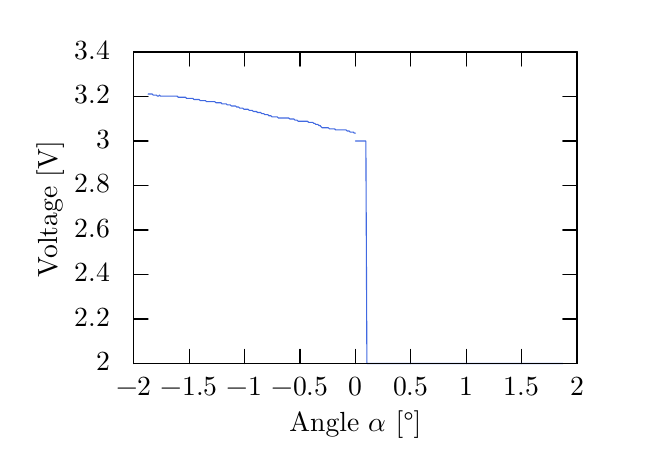
\begin{tikzpicture}[gnuplot]
%% generated with GNUPLOT 5.2p5a (Gentoo revision r0) (Lua 5.1; terminal rev. 99 , script rev. 107)
%% Mi 01 Mai 2019 12:59:13 CEST
\path (0.000,0.000) rectangle (7.500,5.250);
\gpcolor{color=gp lt color border}
\gpsetlinetype{gp lt border}
\gpsetdashtype{gp dt solid}
\gpsetlinewidth{1.00}
\draw[gp path] (1.320,0.985)--(1.500,0.985);
\draw[gp path] (6.947,0.985)--(6.767,0.985);
\node[gp node right] at (1.136,0.985) {$2$};
\draw[gp path] (1.320,1.550)--(1.500,1.550);
\draw[gp path] (6.947,1.550)--(6.767,1.550);
\node[gp node right] at (1.136,1.550) {$2.2$};
\draw[gp path] (1.320,2.115)--(1.500,2.115);
\draw[gp path] (6.947,2.115)--(6.767,2.115);
\node[gp node right] at (1.136,2.115) {$2.4$};
\draw[gp path] (1.320,2.680)--(1.500,2.680);
\draw[gp path] (6.947,2.680)--(6.767,2.680);
\node[gp node right] at (1.136,2.680) {$2.6$};
\draw[gp path] (1.320,3.246)--(1.500,3.246);
\draw[gp path] (6.947,3.246)--(6.767,3.246);
\node[gp node right] at (1.136,3.246) {$2.8$};
\draw[gp path] (1.320,3.811)--(1.500,3.811);
\draw[gp path] (6.947,3.811)--(6.767,3.811);
\node[gp node right] at (1.136,3.811) {$3$};
\draw[gp path] (1.320,4.376)--(1.500,4.376);
\draw[gp path] (6.947,4.376)--(6.767,4.376);
\node[gp node right] at (1.136,4.376) {$3.2$};
\draw[gp path] (1.320,4.941)--(1.500,4.941);
\draw[gp path] (6.947,4.941)--(6.767,4.941);
\node[gp node right] at (1.136,4.941) {$3.4$};
\draw[gp path] (1.320,0.985)--(1.320,1.165);
\draw[gp path] (1.320,4.941)--(1.320,4.761);
\node[gp node center] at (1.320,0.677) {$-2$};
\draw[gp path] (2.023,0.985)--(2.023,1.165);
\draw[gp path] (2.023,4.941)--(2.023,4.761);
\node[gp node center] at (2.023,0.677) {$-1.5$};
\draw[gp path] (2.727,0.985)--(2.727,1.165);
\draw[gp path] (2.727,4.941)--(2.727,4.761);
\node[gp node center] at (2.727,0.677) {$-1$};
\draw[gp path] (3.430,0.985)--(3.430,1.165);
\draw[gp path] (3.430,4.941)--(3.430,4.761);
\node[gp node center] at (3.430,0.677) {$-0.5$};
\draw[gp path] (4.134,0.985)--(4.134,1.165);
\draw[gp path] (4.134,4.941)--(4.134,4.761);
\node[gp node center] at (4.134,0.677) {$0$};
\draw[gp path] (4.837,0.985)--(4.837,1.165);
\draw[gp path] (4.837,4.941)--(4.837,4.761);
\node[gp node center] at (4.837,0.677) {$0.5$};
\draw[gp path] (5.540,0.985)--(5.540,1.165);
\draw[gp path] (5.540,4.941)--(5.540,4.761);
\node[gp node center] at (5.540,0.677) {$1$};
\draw[gp path] (6.244,0.985)--(6.244,1.165);
\draw[gp path] (6.244,4.941)--(6.244,4.761);
\node[gp node center] at (6.244,0.677) {$1.5$};
\draw[gp path] (6.947,0.985)--(6.947,1.165);
\draw[gp path] (6.947,4.941)--(6.947,4.761);
\node[gp node center] at (6.947,0.677) {$2$};
\draw[gp path] (1.320,4.941)--(1.320,0.985)--(6.947,0.985)--(6.947,4.941)--cycle;
\node[gp node center,rotate=-270] at (0.276,2.963) {Voltage [V]};
\node[gp node center] at (4.133,0.215) {Angle $\alpha$ [°]};
\gpcolor{rgb color={0.255,0.412,0.882}}
\draw[gp path] (4.134,3.910)--(4.120,3.910)--(4.107,3.924)--(4.094,3.924)--(4.081,3.924)%
  --(4.067,3.924)--(4.054,3.938)--(4.041,3.938)--(4.028,3.938)--(4.014,3.952)--(4.001,3.952)%
  --(3.988,3.952)--(3.975,3.952)--(3.961,3.952)--(3.948,3.952)--(3.935,3.952)--(3.922,3.952)%
  --(3.909,3.952)--(3.895,3.952)--(3.882,3.952)--(3.869,3.965)--(3.856,3.965)--(3.842,3.965)%
  --(3.829,3.965)--(3.816,3.965)--(3.803,3.965)--(3.789,3.979)--(3.776,3.979)--(3.763,3.979)%
  --(3.750,3.979)--(3.736,3.979)--(3.723,3.979)--(3.710,3.979)--(3.697,3.993)--(3.684,4.007)%
  --(3.670,4.007)--(3.657,4.021)--(3.644,4.021)--(3.631,4.021)--(3.617,4.035)--(3.604,4.035)%
  --(3.591,4.048)--(3.578,4.048)--(3.564,4.048)--(3.551,4.048)--(3.538,4.048)--(3.525,4.062)%
  --(3.511,4.062)--(3.498,4.062)--(3.485,4.062)--(3.472,4.062)--(3.459,4.062)--(3.445,4.062)%
  --(3.432,4.062)--(3.419,4.062)--(3.406,4.062)--(3.392,4.076)--(3.379,4.076)--(3.366,4.076)%
  --(3.353,4.090)--(3.339,4.090)--(3.326,4.090)--(3.313,4.090)--(3.300,4.090)--(3.286,4.103)%
  --(3.273,4.103)--(3.260,4.103)--(3.247,4.103)--(3.234,4.103)--(3.220,4.103)--(3.207,4.103)%
  --(3.194,4.103)--(3.181,4.103)--(3.167,4.103)--(3.154,4.103)--(3.141,4.117)--(3.128,4.117)%
  --(3.114,4.117)--(3.101,4.117)--(3.088,4.117)--(3.075,4.117)--(3.061,4.131)--(3.048,4.131)%
  --(3.035,4.131)--(3.022,4.145)--(3.009,4.145)--(2.995,4.145)--(2.982,4.145)--(2.969,4.159)%
  --(2.956,4.159)--(2.942,4.159)--(2.929,4.173)--(2.916,4.173)--(2.903,4.173)--(2.889,4.173)%
  --(2.876,4.186)--(2.863,4.186)--(2.850,4.186)--(2.836,4.186)--(2.823,4.200)--(2.810,4.200)%
  --(2.797,4.200)--(2.784,4.200)--(2.770,4.214)--(2.757,4.214)--(2.744,4.214)--(2.731,4.214)%
  --(2.717,4.214)--(2.704,4.228)--(2.691,4.228)--(2.678,4.228)--(2.664,4.228)--(2.651,4.242)%
  --(2.638,4.242)--(2.625,4.242)--(2.612,4.255)--(2.598,4.255)--(2.585,4.255)--(2.572,4.255)%
  --(2.559,4.255)--(2.545,4.269)--(2.532,4.269)--(2.519,4.269)--(2.506,4.269)--(2.492,4.283)%
  --(2.479,4.283)--(2.466,4.283)--(2.453,4.283)--(2.439,4.283)--(2.426,4.297)--(2.413,4.297)%
  --(2.400,4.297)--(2.387,4.297)--(2.373,4.297)--(2.360,4.297)--(2.347,4.311)--(2.334,4.311)%
  --(2.320,4.311)--(2.307,4.311)--(2.294,4.311)--(2.281,4.311)--(2.267,4.311)--(2.254,4.311)%
  --(2.241,4.311)--(2.228,4.324)--(2.214,4.324)--(2.201,4.324)--(2.188,4.324)--(2.175,4.324)%
  --(2.162,4.324)--(2.148,4.338)--(2.135,4.338)--(2.122,4.338)--(2.109,4.338)--(2.095,4.338)%
  --(2.082,4.338)--(2.069,4.352)--(2.056,4.352)--(2.042,4.352)--(2.029,4.352)--(2.016,4.352)%
  --(2.003,4.352)--(1.989,4.352)--(1.976,4.366)--(1.963,4.366)--(1.950,4.366)--(1.937,4.366)%
  --(1.923,4.366)--(1.910,4.366)--(1.897,4.366)--(1.884,4.366)--(1.870,4.380)--(1.857,4.380)%
  --(1.844,4.380)--(1.831,4.380)--(1.817,4.380)--(1.804,4.380)--(1.791,4.380)--(1.778,4.380)%
  --(1.764,4.380)--(1.751,4.380)--(1.738,4.380)--(1.725,4.380)--(1.712,4.380)--(1.698,4.380)%
  --(1.685,4.380)--(1.672,4.380)--(1.659,4.380)--(1.645,4.394)--(1.632,4.380)--(1.619,4.380)%
  --(1.606,4.394)--(1.592,4.394)--(1.579,4.394)--(1.566,4.394)--(1.553,4.407)--(1.539,4.407)%
  --(1.526,4.407)--(1.513,4.407)--(1.500,4.407);
\draw[gp path] (4.134,3.811)--(4.147,3.811)--(4.160,3.811)--(4.173,3.811)--(4.186,3.811)%
  --(4.200,3.811)--(4.213,3.811)--(4.226,3.811)--(4.239,3.811)--(4.253,3.811)--(4.266,3.811)%
  --(4.279,0.985)--(4.292,0.985)--(4.306,0.985)--(4.319,0.985)--(4.332,0.985)--(4.345,0.985)%
  --(4.358,0.985)--(4.372,0.985)--(4.385,0.985)--(4.398,0.985)--(4.411,0.985)--(4.425,0.985)%
  --(4.438,0.985)--(4.451,0.985)--(4.464,0.985)--(4.478,0.985)--(4.491,0.985)--(4.504,0.985)%
  --(4.517,0.985)--(4.531,0.985)--(4.544,0.985)--(4.557,0.985)--(4.570,0.985)--(4.583,0.985)%
  --(4.597,0.985)--(4.610,0.985)--(4.623,0.985)--(4.636,0.985)--(4.650,0.985)--(4.663,0.985)%
  --(4.676,0.985)--(4.689,0.985)--(4.703,0.985)--(4.716,0.985)--(4.729,0.985)--(4.742,0.985)%
  --(4.756,0.985)--(4.769,0.985)--(4.782,0.985)--(4.795,0.985)--(4.808,0.985)--(4.822,0.985)%
  --(4.835,0.985)--(4.848,0.985)--(4.861,0.985)--(4.875,0.985)--(4.888,0.985)--(4.901,0.985)%
  --(4.914,0.985)--(4.928,0.985)--(4.941,0.985)--(4.954,0.985)--(4.967,0.985)--(4.981,0.985)%
  --(4.994,0.985)--(5.007,0.985)--(5.020,0.985)--(5.033,0.985)--(5.047,0.985)--(5.060,0.985)%
  --(5.073,0.985)--(5.086,0.985)--(5.100,0.985)--(5.113,0.985)--(5.126,0.985)--(5.139,0.985)%
  --(5.153,0.985)--(5.166,0.985)--(5.179,0.985)--(5.192,0.985)--(5.206,0.985)--(5.219,0.985)%
  --(5.232,0.985)--(5.245,0.985)--(5.258,0.985)--(5.272,0.985)--(5.285,0.985)--(5.298,0.985)%
  --(5.311,0.985)--(5.325,0.985)--(5.338,0.985)--(5.351,0.985)--(5.364,0.985)--(5.378,0.985)%
  --(5.391,0.985)--(5.404,0.985)--(5.417,0.985)--(5.431,0.985)--(5.444,0.985)--(5.457,0.985)%
  --(5.470,0.985)--(5.483,0.985)--(5.497,0.985)--(5.510,0.985)--(5.523,0.985)--(5.536,0.985)%
  --(5.550,0.985)--(5.563,0.985)--(5.576,0.985)--(5.589,0.985)--(5.603,0.985)--(5.616,0.985)%
  --(5.629,0.985)--(5.642,0.985)--(5.655,0.985)--(5.669,0.985)--(5.682,0.985)--(5.695,0.985)%
  --(5.708,0.985)--(5.722,0.985)--(5.735,0.985)--(5.748,0.985)--(5.761,0.985)--(5.775,0.985)%
  --(5.788,0.985)--(5.801,0.985)--(5.814,0.985)--(5.828,0.985)--(5.841,0.985)--(5.854,0.985)%
  --(5.867,0.985)--(5.880,0.985)--(5.894,0.985)--(5.907,0.985)--(5.920,0.985)--(5.933,0.985)%
  --(5.947,0.985)--(5.960,0.985)--(5.973,0.985)--(5.986,0.985)--(6.000,0.985)--(6.013,0.985)%
  --(6.026,0.985)--(6.039,0.985)--(6.053,0.985)--(6.066,0.985)--(6.079,0.985)--(6.092,0.985)%
  --(6.105,0.985)--(6.119,0.985)--(6.132,0.985)--(6.145,0.985)--(6.158,0.985)--(6.172,0.985)%
  --(6.185,0.985)--(6.198,0.985)--(6.211,0.985)--(6.225,0.985)--(6.238,0.985)--(6.251,0.985)%
  --(6.264,0.985)--(6.278,0.985)--(6.291,0.985)--(6.304,0.985)--(6.317,0.985)--(6.330,0.985)%
  --(6.344,0.985)--(6.357,0.985)--(6.370,0.985)--(6.383,0.985)--(6.397,0.985)--(6.410,0.985)%
  --(6.423,0.985)--(6.436,0.985)--(6.450,0.985)--(6.463,0.985)--(6.476,0.985)--(6.489,0.985)%
  --(6.503,0.985)--(6.516,0.985)--(6.529,0.985)--(6.542,0.985)--(6.555,0.985)--(6.569,0.985)%
  --(6.582,0.985)--(6.595,0.985)--(6.608,0.985)--(6.622,0.985)--(6.635,0.985)--(6.648,0.985)%
  --(6.661,0.985)--(6.675,0.985)--(6.688,0.985)--(6.701,0.985)--(6.714,0.985)--(6.728,0.985)%
  --(6.741,0.985)--(6.754,0.985)--(6.767,0.985);
\gpcolor{color=gp lt color border}
\draw[gp path] (1.320,4.941)--(1.320,0.985)--(6.947,0.985)--(6.947,4.941)--cycle;
%% coordinates of the plot area
\gpdefrectangularnode{gp plot 1}{\pgfpoint{1.320cm}{0.985cm}}{\pgfpoint{6.947cm}{4.941cm}}
\end{tikzpicture}
%% gnuplot variables

		\caption{Laser wavenlength 850 nm}
	\end{subfigure}
	\caption{The reflectivity of the mirror at two different laser wavelenghts}
\end{figure}
\begin{figure}
	\begin{tikzpicture}[gnuplot]
%% generated with GNUPLOT 5.2p5a (Gentoo revision r0) (Lua 5.1; terminal rev. 99 , script rev. 107)
%% Mi 24 Apr 2019 10:03:58 CEST
\path (0.000,0.000) rectangle (12.500,8.750);
\gpcolor{color=gp lt color border}
\gpsetlinetype{gp lt border}
\gpsetdashtype{gp dt solid}
\gpsetlinewidth{1.00}
\draw[gp path] (1.320,0.985)--(1.500,0.985);
\draw[gp path] (11.947,0.985)--(11.767,0.985);
\node[gp node right] at (1.136,0.985) {$0.2$};
\draw[gp path] (1.320,1.731)--(1.500,1.731);
\draw[gp path] (11.947,1.731)--(11.767,1.731);
\node[gp node right] at (1.136,1.731) {$0.4$};
\draw[gp path] (1.320,2.476)--(1.500,2.476);
\draw[gp path] (11.947,2.476)--(11.767,2.476);
\node[gp node right] at (1.136,2.476) {$0.6$};
\draw[gp path] (1.320,3.222)--(1.500,3.222);
\draw[gp path] (11.947,3.222)--(11.767,3.222);
\node[gp node right] at (1.136,3.222) {$0.8$};
\draw[gp path] (1.320,3.967)--(1.500,3.967);
\draw[gp path] (11.947,3.967)--(11.767,3.967);
\node[gp node right] at (1.136,3.967) {$1$};
\draw[gp path] (1.320,4.713)--(1.500,4.713);
\draw[gp path] (11.947,4.713)--(11.767,4.713);
\node[gp node right] at (1.136,4.713) {$1.2$};
\draw[gp path] (1.320,5.459)--(1.500,5.459);
\draw[gp path] (11.947,5.459)--(11.767,5.459);
\node[gp node right] at (1.136,5.459) {$1.4$};
\draw[gp path] (1.320,6.204)--(1.500,6.204);
\draw[gp path] (11.947,6.204)--(11.767,6.204);
\node[gp node right] at (1.136,6.204) {$1.6$};
\draw[gp path] (1.320,6.950)--(1.500,6.950);
\draw[gp path] (11.947,6.950)--(11.767,6.950);
\node[gp node right] at (1.136,6.950) {$1.8$};
\draw[gp path] (1.320,7.695)--(1.500,7.695);
\draw[gp path] (11.947,7.695)--(11.767,7.695);
\node[gp node right] at (1.136,7.695) {$2$};
\draw[gp path] (1.320,8.441)--(1.500,8.441);
\draw[gp path] (11.947,8.441)--(11.767,8.441);
\node[gp node right] at (1.136,8.441) {$2.2$};
\draw[gp path] (1.320,0.985)--(1.320,1.165);
\draw[gp path] (1.320,8.441)--(1.320,8.261);
\node[gp node center] at (1.320,0.677) {$-2$};
\draw[gp path] (2.383,0.985)--(2.383,1.165);
\draw[gp path] (2.383,8.441)--(2.383,8.261);
\node[gp node center] at (2.383,0.677) {$-1.8$};
\draw[gp path] (3.445,0.985)--(3.445,1.165);
\draw[gp path] (3.445,8.441)--(3.445,8.261);
\node[gp node center] at (3.445,0.677) {$-1.6$};
\draw[gp path] (4.508,0.985)--(4.508,1.165);
\draw[gp path] (4.508,8.441)--(4.508,8.261);
\node[gp node center] at (4.508,0.677) {$-1.4$};
\draw[gp path] (5.571,0.985)--(5.571,1.165);
\draw[gp path] (5.571,8.441)--(5.571,8.261);
\node[gp node center] at (5.571,0.677) {$-1.2$};
\draw[gp path] (6.633,0.985)--(6.633,1.165);
\draw[gp path] (6.633,8.441)--(6.633,8.261);
\node[gp node center] at (6.633,0.677) {$-1$};
\draw[gp path] (7.696,0.985)--(7.696,1.165);
\draw[gp path] (7.696,8.441)--(7.696,8.261);
\node[gp node center] at (7.696,0.677) {$-0.8$};
\draw[gp path] (8.759,0.985)--(8.759,1.165);
\draw[gp path] (8.759,8.441)--(8.759,8.261);
\node[gp node center] at (8.759,0.677) {$-0.6$};
\draw[gp path] (9.822,0.985)--(9.822,1.165);
\draw[gp path] (9.822,8.441)--(9.822,8.261);
\node[gp node center] at (9.822,0.677) {$-0.4$};
\draw[gp path] (10.884,0.985)--(10.884,1.165);
\draw[gp path] (10.884,8.441)--(10.884,8.261);
\node[gp node center] at (10.884,0.677) {$-0.2$};
\draw[gp path] (11.947,0.985)--(11.947,1.165);
\draw[gp path] (11.947,8.441)--(11.947,8.261);
\node[gp node center] at (11.947,0.677) {$0$};
\draw[gp path] (1.320,8.441)--(1.320,0.985)--(11.947,0.985)--(11.947,8.441)--cycle;
\node[gp node center,rotate=-270] at (0.276,4.713) {Voltage [V]};
\node[gp node center] at (6.633,0.215) {Angle $\alpha$ [°]};
\gpcolor{rgb color={0.580,0.000,0.827}}
\draw[gp path] (11.947,7.911)--(11.897,7.929)--(11.847,7.929)--(11.797,7.929)--(11.747,7.947)%
  --(11.697,7.947)--(11.647,7.947)--(11.597,7.965)--(11.547,7.965)--(11.497,7.965)--(11.447,7.965)%
  --(11.397,7.965)--(11.347,7.947)--(11.297,7.947)--(11.247,7.929)--(11.197,7.929)--(11.147,7.929)%
  --(11.097,7.911)--(11.047,7.892)--(10.997,7.892)--(10.947,7.874)--(10.897,7.874)--(10.847,7.874)%
  --(10.797,7.874)--(10.747,7.874)--(10.697,7.874)--(10.647,7.892)--(10.597,7.892)--(10.547,7.892)%
  --(10.497,7.911)--(10.447,7.929)--(10.397,7.947)--(10.347,7.965)--(10.297,7.983)--(10.247,8.001)%
  --(10.197,8.001)--(10.147,8.020)--(10.097,8.020)--(10.047,8.038)--(9.997,8.038)--(9.947,8.038)%
  --(9.897,8.056)--(9.847,8.056)--(9.797,8.038)--(9.747,8.038)--(9.697,8.038)--(9.647,8.038)%
  --(9.597,8.020)--(9.548,8.020)--(9.498,8.038)--(9.448,8.038)--(9.398,8.038)--(9.348,8.038)%
  --(9.298,8.038)--(9.248,8.038)--(9.198,8.038)--(9.148,8.038)--(9.098,8.038)--(9.048,8.020)%
  --(8.998,8.020)--(8.948,8.020)--(8.898,8.020)--(8.848,8.001)--(8.798,8.001)--(8.748,8.001)%
  --(8.698,7.983)--(8.648,7.965)--(8.598,7.965)--(8.548,7.965)--(8.498,7.965)--(8.448,7.947)%
  --(8.398,7.929)--(8.348,7.929)--(8.298,7.911)--(8.248,7.892)--(8.198,7.892)--(8.148,7.874)%
  --(8.098,7.837)--(8.048,7.819)--(7.998,7.783)--(7.948,7.765)--(7.898,7.728)--(7.848,7.673)%
  --(7.798,7.619)--(7.748,7.564)--(7.698,7.491)--(7.648,7.437)--(7.598,7.364)--(7.548,7.273)%
  --(7.498,7.182)--(7.448,7.090)--(7.398,6.999)--(7.348,6.890)--(7.298,6.799)--(7.248,6.671)%
  --(7.198,6.562)--(7.148,6.453)--(7.098,6.325)--(7.048,6.216)--(6.998,6.107)--(6.948,5.979)%
  --(6.898,5.870)--(6.848,5.742)--(6.798,5.614)--(6.748,5.487)--(6.698,5.359)--(6.648,5.232)%
  --(6.598,5.104)--(6.548,4.995)--(6.498,4.867)--(6.448,4.740)--(6.398,4.612)--(6.348,4.485)%
  --(6.298,4.357)--(6.248,4.248)--(6.198,4.139)--(6.148,4.029)--(6.098,3.938)--(6.048,3.847)%
  --(5.998,3.774)--(5.948,3.701)--(5.898,3.629)--(5.848,3.555)--(5.798,3.483)--(5.748,3.410)%
  --(5.698,3.337)--(5.648,3.282)--(5.598,3.209)--(5.548,3.155)--(5.498,3.100)--(5.448,3.045)%
  --(5.398,2.991)--(5.348,2.936)--(5.298,2.881)--(5.248,2.827)--(5.198,2.790)--(5.148,2.736)%
  --(5.098,2.681)--(5.048,2.626)--(4.998,2.590)--(4.948,2.535)--(4.898,2.499)--(4.849,2.444)%
  --(4.799,2.408)--(4.749,2.371)--(4.699,2.335)--(4.649,2.298)--(4.599,2.262)--(4.549,2.225)%
  --(4.499,2.189)--(4.449,2.153)--(4.399,2.116)--(4.349,2.080)--(4.299,2.043)--(4.249,2.007)%
  --(4.199,1.970)--(4.149,1.952)--(4.099,1.916)--(4.049,1.879)--(3.999,1.861)--(3.949,1.825)%
  --(3.899,1.806)--(3.849,1.770)--(3.799,1.752)--(3.749,1.715)--(3.699,1.697)--(3.649,1.661)%
  --(3.599,1.642)--(3.549,1.624)--(3.499,1.606)--(3.449,1.570)--(3.399,1.551)--(3.349,1.533)%
  --(3.299,1.515)--(3.249,1.496)--(3.199,1.479)--(3.149,1.460)--(3.099,1.442)--(3.049,1.424)%
  --(2.999,1.406)--(2.949,1.387)--(2.899,1.369)--(2.849,1.351)--(2.799,1.333)--(2.749,1.315)%
  --(2.699,1.315)--(2.649,1.296)--(2.599,1.278)--(2.549,1.260)--(2.499,1.241)--(2.449,1.241)%
  --(2.399,1.223)--(2.349,1.205)--(2.299,1.187)--(2.249,1.187)--(2.199,1.169)--(2.149,1.151)%
  --(2.099,1.151)--(2.049,1.132)--(1.999,1.114);
\gpcolor{color=gp lt color border}
\draw[gp path] (1.320,8.441)--(1.320,0.985)--(11.947,0.985)--(11.947,8.441)--cycle;
%% coordinates of the plot area
\gpdefrectangularnode{gp plot 1}{\pgfpoint{1.320cm}{0.985cm}}{\pgfpoint{11.947cm}{8.441cm}}
\end{tikzpicture}
%% gnuplot variables

	\caption{The reflectivity of the uncoated prism}
\end{figure}
\begin{figure}
	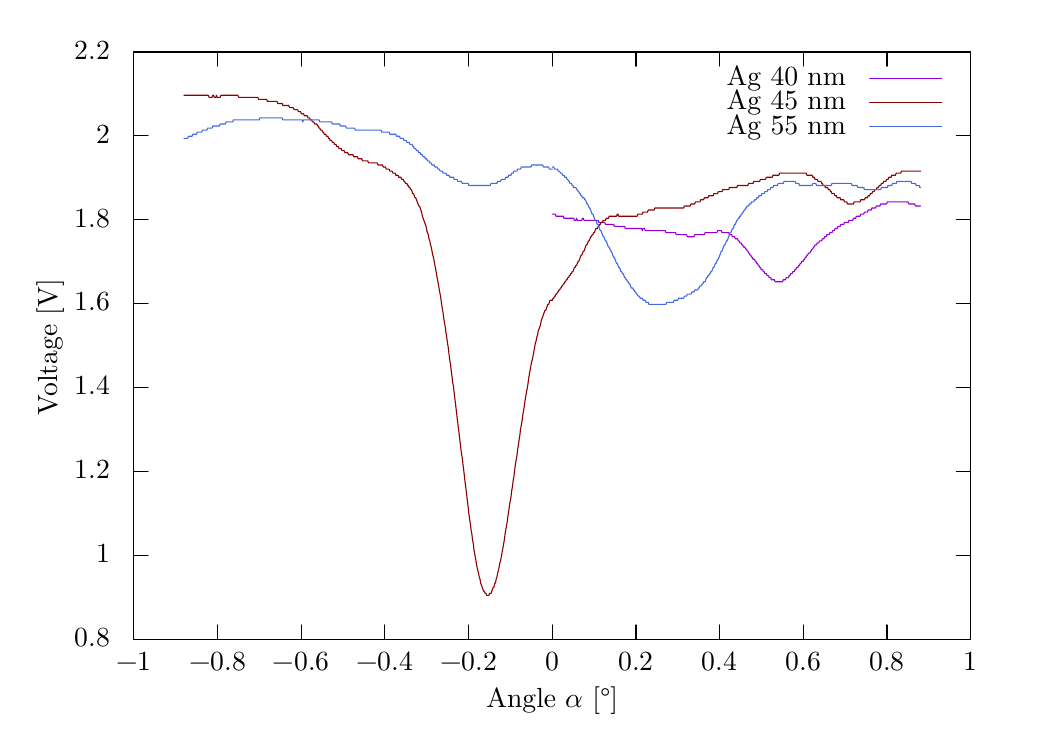
\begin{tikzpicture}[gnuplot]
%% generated with GNUPLOT 5.2p5a (Gentoo revision r0) (Lua 5.1; terminal rev. 99 , script rev. 107)
%% Mi 24 Apr 2019 10:58:09 CEST
\path (0.000,0.000) rectangle (12.500,8.750);
\gpcolor{color=gp lt color border}
\gpsetlinetype{gp lt border}
\gpsetdashtype{gp dt solid}
\gpsetlinewidth{1.00}
\draw[gp path] (1.320,0.985)--(1.500,0.985);
\draw[gp path] (11.947,0.985)--(11.767,0.985);
\node[gp node right] at (1.136,0.985) {$0.8$};
\draw[gp path] (1.320,2.050)--(1.500,2.050);
\draw[gp path] (11.947,2.050)--(11.767,2.050);
\node[gp node right] at (1.136,2.050) {$1$};
\draw[gp path] (1.320,3.115)--(1.500,3.115);
\draw[gp path] (11.947,3.115)--(11.767,3.115);
\node[gp node right] at (1.136,3.115) {$1.2$};
\draw[gp path] (1.320,4.180)--(1.500,4.180);
\draw[gp path] (11.947,4.180)--(11.767,4.180);
\node[gp node right] at (1.136,4.180) {$1.4$};
\draw[gp path] (1.320,5.246)--(1.500,5.246);
\draw[gp path] (11.947,5.246)--(11.767,5.246);
\node[gp node right] at (1.136,5.246) {$1.6$};
\draw[gp path] (1.320,6.311)--(1.500,6.311);
\draw[gp path] (11.947,6.311)--(11.767,6.311);
\node[gp node right] at (1.136,6.311) {$1.8$};
\draw[gp path] (1.320,7.376)--(1.500,7.376);
\draw[gp path] (11.947,7.376)--(11.767,7.376);
\node[gp node right] at (1.136,7.376) {$2$};
\draw[gp path] (1.320,8.441)--(1.500,8.441);
\draw[gp path] (11.947,8.441)--(11.767,8.441);
\node[gp node right] at (1.136,8.441) {$2.2$};
\draw[gp path] (1.320,0.985)--(1.320,1.165);
\draw[gp path] (1.320,8.441)--(1.320,8.261);
\node[gp node center] at (1.320,0.677) {$-1$};
\draw[gp path] (2.383,0.985)--(2.383,1.165);
\draw[gp path] (2.383,8.441)--(2.383,8.261);
\node[gp node center] at (2.383,0.677) {$-0.8$};
\draw[gp path] (3.445,0.985)--(3.445,1.165);
\draw[gp path] (3.445,8.441)--(3.445,8.261);
\node[gp node center] at (3.445,0.677) {$-0.6$};
\draw[gp path] (4.508,0.985)--(4.508,1.165);
\draw[gp path] (4.508,8.441)--(4.508,8.261);
\node[gp node center] at (4.508,0.677) {$-0.4$};
\draw[gp path] (5.571,0.985)--(5.571,1.165);
\draw[gp path] (5.571,8.441)--(5.571,8.261);
\node[gp node center] at (5.571,0.677) {$-0.2$};
\draw[gp path] (6.634,0.985)--(6.634,1.165);
\draw[gp path] (6.634,8.441)--(6.634,8.261);
\node[gp node center] at (6.634,0.677) {$0$};
\draw[gp path] (7.696,0.985)--(7.696,1.165);
\draw[gp path] (7.696,8.441)--(7.696,8.261);
\node[gp node center] at (7.696,0.677) {$0.2$};
\draw[gp path] (8.759,0.985)--(8.759,1.165);
\draw[gp path] (8.759,8.441)--(8.759,8.261);
\node[gp node center] at (8.759,0.677) {$0.4$};
\draw[gp path] (9.822,0.985)--(9.822,1.165);
\draw[gp path] (9.822,8.441)--(9.822,8.261);
\node[gp node center] at (9.822,0.677) {$0.6$};
\draw[gp path] (10.884,0.985)--(10.884,1.165);
\draw[gp path] (10.884,8.441)--(10.884,8.261);
\node[gp node center] at (10.884,0.677) {$0.8$};
\draw[gp path] (11.947,0.985)--(11.947,1.165);
\draw[gp path] (11.947,8.441)--(11.947,8.261);
\node[gp node center] at (11.947,0.677) {$1$};
\draw[gp path] (1.320,8.441)--(1.320,0.985)--(11.947,0.985)--(11.947,8.441)--cycle;
\node[gp node center,rotate=-270] at (0.276,4.713) {Voltage [V]};
\node[gp node center] at (6.633,0.215) {Angle $\alpha$ [°]};
\node[gp node right] at (10.479,8.107) {Ag 40 nm};
\gpcolor{rgb color={0.580,0.000,0.827}}
\draw[gp path] (10.663,8.107)--(11.579,8.107);
\draw[gp path] (6.634,6.382)--(6.643,6.382)--(6.652,6.382)--(6.662,6.382)--(6.671,6.382)%
  --(6.680,6.355)--(6.690,6.355)--(6.699,6.355)--(6.708,6.355)--(6.718,6.355)--(6.727,6.355)%
  --(6.737,6.355)--(6.746,6.355)--(6.755,6.355)--(6.765,6.355)--(6.774,6.355)--(6.783,6.329)%
  --(6.793,6.329)--(6.802,6.329)--(6.812,6.329)--(6.821,6.329)--(6.830,6.329)--(6.840,6.329)%
  --(6.849,6.329)--(6.858,6.329)--(6.868,6.329)--(6.877,6.329)--(6.887,6.329)--(6.896,6.329)%
  --(6.905,6.329)--(6.915,6.303)--(6.924,6.303)--(6.933,6.303)--(6.943,6.329)--(6.952,6.303)%
  --(6.962,6.303)--(6.971,6.303)--(6.980,6.303)--(6.990,6.303)--(6.999,6.303)--(7.008,6.303)%
  --(7.018,6.329)--(7.027,6.329)--(7.037,6.303)--(7.046,6.303)--(7.055,6.303)--(7.065,6.303)%
  --(7.074,6.303)--(7.083,6.303)--(7.093,6.303)--(7.102,6.303)--(7.112,6.303)--(7.121,6.303)%
  --(7.130,6.303)--(7.140,6.303)--(7.149,6.303)--(7.158,6.303)--(7.168,6.303)--(7.177,6.303)%
  --(7.187,6.303)--(7.196,6.303)--(7.205,6.303)--(7.215,6.303)--(7.224,6.277)--(7.233,6.277)%
  --(7.243,6.277)--(7.252,6.277)--(7.261,6.277)--(7.271,6.277)--(7.280,6.277)--(7.290,6.277)%
  --(7.299,6.277)--(7.308,6.252)--(7.318,6.252)--(7.327,6.252)--(7.336,6.252)--(7.346,6.252)%
  --(7.355,6.252)--(7.365,6.252)--(7.374,6.252)--(7.383,6.252)--(7.393,6.252)--(7.402,6.252)%
  --(7.411,6.252)--(7.421,6.226)--(7.430,6.226)--(7.440,6.226)--(7.449,6.226)--(7.458,6.226)%
  --(7.468,6.226)--(7.477,6.226)--(7.486,6.226)--(7.496,6.226)--(7.505,6.226)--(7.515,6.226)%
  --(7.524,6.226)--(7.533,6.226)--(7.543,6.226)--(7.552,6.226)--(7.561,6.199)--(7.571,6.199)%
  --(7.580,6.199)--(7.590,6.199)--(7.599,6.199)--(7.608,6.199)--(7.618,6.199)--(7.627,6.199)%
  --(7.636,6.199)--(7.646,6.199)--(7.655,6.199)--(7.665,6.199)--(7.674,6.199)--(7.683,6.199)%
  --(7.693,6.199)--(7.702,6.199)--(7.711,6.199)--(7.721,6.199)--(7.730,6.199)--(7.740,6.199)%
  --(7.749,6.199)--(7.758,6.199)--(7.768,6.199)--(7.777,6.173)--(7.786,6.199)--(7.796,6.199)%
  --(7.805,6.199)--(7.814,6.173)--(7.824,6.173)--(7.833,6.173)--(7.843,6.173)--(7.852,6.173)%
  --(7.861,6.173)--(7.871,6.173)--(7.880,6.173)--(7.889,6.173)--(7.899,6.173)--(7.908,6.173)%
  --(7.918,6.173)--(7.927,6.173)--(7.936,6.173)--(7.946,6.173)--(7.955,6.173)--(7.964,6.173)%
  --(7.974,6.173)--(7.983,6.173)--(7.993,6.173)--(8.002,6.173)--(8.011,6.173)--(8.021,6.173)%
  --(8.030,6.173)--(8.039,6.173)--(8.049,6.173)--(8.058,6.173)--(8.068,6.173)--(8.077,6.147)%
  --(8.086,6.147)--(8.096,6.147)--(8.105,6.147)--(8.114,6.147)--(8.124,6.147)--(8.133,6.147)%
  --(8.143,6.147)--(8.152,6.147)--(8.161,6.147)--(8.171,6.147)--(8.180,6.147)--(8.189,6.147)%
  --(8.199,6.147)--(8.208,6.121)--(8.218,6.121)--(8.227,6.121)--(8.236,6.121)--(8.246,6.121)%
  --(8.255,6.121)--(8.264,6.121)--(8.274,6.121)--(8.283,6.121)--(8.293,6.121)--(8.302,6.121)%
  --(8.311,6.121)--(8.321,6.121)--(8.330,6.121)--(8.339,6.121)--(8.349,6.095)--(8.358,6.095)%
  --(8.368,6.095)--(8.377,6.095)--(8.386,6.095)--(8.396,6.095)--(8.405,6.095)--(8.414,6.095)%
  --(8.424,6.095)--(8.433,6.095)--(8.442,6.121)--(8.452,6.121)--(8.461,6.121)--(8.471,6.121)%
  --(8.480,6.121)--(8.489,6.121)--(8.499,6.121)--(8.508,6.121)--(8.517,6.121)--(8.527,6.121)%
  --(8.536,6.121)--(8.546,6.121)--(8.555,6.121)--(8.564,6.121)--(8.574,6.147)--(8.583,6.147)%
  --(8.592,6.147)--(8.602,6.147)--(8.611,6.147)--(8.621,6.147)--(8.630,6.147)--(8.639,6.147)%
  --(8.649,6.147)--(8.658,6.147)--(8.667,6.147)--(8.677,6.147)--(8.686,6.147)--(8.696,6.147)%
  --(8.705,6.147)--(8.714,6.147)--(8.724,6.147)--(8.733,6.173)--(8.742,6.173)--(8.752,6.173)%
  --(8.761,6.173)--(8.771,6.173)--(8.780,6.173)--(8.789,6.147)--(8.799,6.147)--(8.808,6.147)%
  --(8.817,6.147)--(8.827,6.147)--(8.836,6.147)--(8.846,6.147)--(8.855,6.147)--(8.864,6.147)%
  --(8.874,6.147)--(8.883,6.121)--(8.892,6.121)--(8.902,6.121)--(8.911,6.121)--(8.921,6.095)%
  --(8.930,6.095)--(8.939,6.095)--(8.949,6.095)--(8.958,6.069)--(8.967,6.069)--(8.977,6.069)%
  --(8.986,6.069)--(8.995,6.043)--(9.005,6.043)--(9.014,6.017)--(9.024,6.017)--(9.033,6.017)%
  --(9.042,5.991)--(9.052,5.991)--(9.061,5.965)--(9.070,5.965)--(9.080,5.965)--(9.089,5.939)%
  --(9.099,5.939)--(9.108,5.913)--(9.117,5.913)--(9.127,5.887)--(9.136,5.887)--(9.145,5.861)%
  --(9.155,5.861)--(9.164,5.835)--(9.174,5.835)--(9.183,5.809)--(9.192,5.809)--(9.202,5.809)%
  --(9.211,5.783)--(9.220,5.783)--(9.230,5.757)--(9.239,5.757)--(9.249,5.731)--(9.258,5.731)%
  --(9.267,5.705)--(9.277,5.705)--(9.286,5.679)--(9.295,5.679)--(9.305,5.679)--(9.314,5.652)%
  --(9.324,5.652)--(9.333,5.627)--(9.342,5.627)--(9.352,5.627)--(9.361,5.601)--(9.370,5.601)%
  --(9.380,5.601)--(9.389,5.575)--(9.399,5.575)--(9.408,5.575)--(9.417,5.549)--(9.427,5.549)%
  --(9.436,5.549)--(9.445,5.549)--(9.455,5.549)--(9.464,5.523)--(9.474,5.523)--(9.483,5.523)%
  --(9.492,5.523)--(9.502,5.523)--(9.511,5.523)--(9.520,5.523)--(9.530,5.523)--(9.539,5.523)%
  --(9.549,5.523)--(9.558,5.523)--(9.567,5.549)--(9.577,5.549)--(9.586,5.549)--(9.595,5.549)%
  --(9.605,5.575)--(9.614,5.575)--(9.623,5.575)--(9.633,5.575)--(9.642,5.601)--(9.652,5.601)%
  --(9.661,5.627)--(9.670,5.627)--(9.680,5.627)--(9.689,5.652)--(9.698,5.652)--(9.708,5.652)%
  --(9.717,5.679)--(9.727,5.679)--(9.736,5.705)--(9.745,5.705)--(9.755,5.705)--(9.764,5.731)%
  --(9.773,5.731)--(9.783,5.757)--(9.792,5.757)--(9.802,5.783)--(9.811,5.783)--(9.820,5.783)%
  --(9.830,5.809)--(9.839,5.809)--(9.848,5.835)--(9.858,5.835)--(9.867,5.861)--(9.877,5.861)%
  --(9.886,5.887)--(9.895,5.887)--(9.905,5.887)--(9.914,5.913)--(9.923,5.913)--(9.933,5.939)%
  --(9.942,5.939)--(9.952,5.965)--(9.961,5.965)--(9.970,5.991)--(9.980,5.991)--(9.989,5.991)%
  --(9.998,6.017)--(10.008,6.017)--(10.017,6.017)--(10.027,6.043)--(10.036,6.043)--(10.045,6.043)%
  --(10.055,6.043)--(10.064,6.069)--(10.073,6.069)--(10.083,6.069)--(10.092,6.095)--(10.102,6.095)%
  --(10.111,6.095)--(10.120,6.121)--(10.130,6.121)--(10.139,6.121)--(10.148,6.121)--(10.158,6.147)%
  --(10.167,6.147)--(10.176,6.147)--(10.186,6.147)--(10.195,6.173)--(10.205,6.173)--(10.214,6.173)%
  --(10.223,6.199)--(10.233,6.199)--(10.242,6.199)--(10.251,6.199)--(10.261,6.226)--(10.270,6.226)%
  --(10.280,6.226)--(10.289,6.226)--(10.298,6.252)--(10.308,6.252)--(10.317,6.252)--(10.326,6.252)%
  --(10.336,6.252)--(10.345,6.277)--(10.355,6.277)--(10.364,6.277)--(10.373,6.277)--(10.383,6.277)%
  --(10.392,6.277)--(10.401,6.303)--(10.411,6.303)--(10.420,6.303)--(10.430,6.303)--(10.439,6.303)%
  --(10.448,6.303)--(10.458,6.329)--(10.467,6.329)--(10.476,6.329)--(10.486,6.329)--(10.495,6.355)%
  --(10.505,6.355)--(10.514,6.355)--(10.523,6.355)--(10.533,6.355)--(10.542,6.355)--(10.551,6.382)%
  --(10.561,6.382)--(10.570,6.382)--(10.580,6.382)--(10.589,6.382)--(10.598,6.408)--(10.608,6.408)%
  --(10.617,6.408)--(10.626,6.408)--(10.636,6.408)--(10.645,6.434)--(10.655,6.434)--(10.664,6.434)%
  --(10.673,6.434)--(10.683,6.434)--(10.692,6.460)--(10.701,6.460)--(10.711,6.460)--(10.720,6.460)%
  --(10.730,6.460)--(10.739,6.460)--(10.748,6.485)--(10.758,6.485)--(10.767,6.485)--(10.776,6.485)%
  --(10.786,6.485)--(10.795,6.485)--(10.804,6.511)--(10.814,6.511)--(10.823,6.511)--(10.833,6.511)%
  --(10.842,6.511)--(10.851,6.511)--(10.861,6.511)--(10.870,6.511)--(10.879,6.511)--(10.889,6.538)%
  --(10.898,6.538)--(10.908,6.538)--(10.917,6.538)--(10.926,6.538)--(10.936,6.538)--(10.945,6.538)%
  --(10.954,6.538)--(10.964,6.538)--(10.973,6.538)--(10.983,6.538)--(10.992,6.538)--(11.001,6.538)%
  --(11.011,6.538)--(11.020,6.538)--(11.029,6.538)--(11.039,6.538)--(11.048,6.538)--(11.058,6.538)%
  --(11.067,6.538)--(11.076,6.538)--(11.086,6.538)--(11.095,6.538)--(11.104,6.538)--(11.114,6.538)%
  --(11.123,6.538)--(11.133,6.538)--(11.142,6.538)--(11.151,6.538)--(11.161,6.511)--(11.170,6.511)%
  --(11.179,6.511)--(11.189,6.511)--(11.198,6.511)--(11.208,6.511)--(11.217,6.511)--(11.226,6.511)%
  --(11.236,6.511)--(11.245,6.485)--(11.254,6.485)--(11.264,6.485)--(11.273,6.485)--(11.283,6.485)%
  --(11.292,6.485)--(11.301,6.485)--(11.311,6.485);
\gpcolor{rgb color={0.545,0.000,0.000}}
\draw[gp path] (6.634,5.288)--(6.624,5.288)--(6.615,5.288)--(6.605,5.288)--(6.596,5.262)%
  --(6.587,5.236)--(6.577,5.236)--(6.568,5.210)--(6.559,5.184)--(6.549,5.158)--(6.540,5.158)%
  --(6.530,5.132)--(6.521,5.106)--(6.512,5.080)--(6.502,5.054)--(6.493,5.028)--(6.484,4.976)%
  --(6.474,4.950)--(6.465,4.924)--(6.455,4.898)--(6.446,4.846)--(6.437,4.820)--(6.427,4.768)%
  --(6.418,4.742)--(6.409,4.690)--(6.399,4.637)--(6.390,4.586)--(6.380,4.534)--(6.371,4.507)%
  --(6.362,4.455)--(6.352,4.403)--(6.343,4.351)--(6.334,4.299)--(6.324,4.221)--(6.315,4.169)%
  --(6.305,4.117)--(6.296,4.065)--(6.287,4.013)--(6.277,3.935)--(6.268,3.883)--(6.259,3.831)%
  --(6.249,3.752)--(6.240,3.701)--(6.230,3.648)--(6.221,3.570)--(6.212,3.518)--(6.202,3.440)%
  --(6.193,3.388)--(6.184,3.310)--(6.174,3.258)--(6.165,3.206)--(6.155,3.128)--(6.146,3.050)%
  --(6.137,2.998)--(6.127,2.919)--(6.118,2.868)--(6.109,2.789)--(6.099,2.737)--(6.090,2.686)%
  --(6.080,2.607)--(6.071,2.555)--(6.062,2.477)--(6.052,2.425)--(6.043,2.373)--(6.034,2.321)%
  --(6.024,2.243)--(6.015,2.191)--(6.006,2.139)--(5.996,2.086)--(5.987,2.035)--(5.977,1.983)%
  --(5.968,1.956)--(5.959,1.904)--(5.949,1.853)--(5.940,1.826)--(5.931,1.774)--(5.921,1.748)%
  --(5.912,1.696)--(5.902,1.696)--(5.893,1.644)--(5.884,1.644)--(5.874,1.618)--(5.865,1.592)%
  --(5.856,1.566)--(5.846,1.566)--(5.837,1.566)--(5.827,1.540)--(5.818,1.540)--(5.809,1.540)%
  --(5.799,1.540)--(5.790,1.566)--(5.781,1.566)--(5.771,1.592)--(5.762,1.592)--(5.752,1.618)%
  --(5.743,1.644)--(5.734,1.670)--(5.724,1.696)--(5.715,1.748)--(5.706,1.774)--(5.696,1.826)%
  --(5.687,1.853)--(5.677,1.904)--(5.668,1.956)--(5.659,2.009)--(5.649,2.061)--(5.640,2.112)%
  --(5.631,2.191)--(5.621,2.243)--(5.612,2.321)--(5.602,2.373)--(5.593,2.451)--(5.584,2.503)%
  --(5.574,2.581)--(5.565,2.659)--(5.556,2.737)--(5.546,2.815)--(5.537,2.894)--(5.527,2.971)%
  --(5.518,3.050)--(5.509,3.128)--(5.499,3.206)--(5.490,3.284)--(5.481,3.336)--(5.471,3.414)%
  --(5.462,3.492)--(5.453,3.570)--(5.443,3.648)--(5.434,3.727)--(5.424,3.804)--(5.415,3.883)%
  --(5.406,3.960)--(5.396,4.039)--(5.387,4.117)--(5.378,4.195)--(5.368,4.247)--(5.359,4.325)%
  --(5.349,4.403)--(5.340,4.481)--(5.331,4.534)--(5.321,4.611)--(5.312,4.690)--(5.303,4.742)%
  --(5.293,4.820)--(5.284,4.872)--(5.274,4.950)--(5.265,5.002)--(5.256,5.054)--(5.246,5.132)%
  --(5.237,5.184)--(5.228,5.236)--(5.218,5.314)--(5.209,5.366)--(5.199,5.419)--(5.190,5.470)%
  --(5.181,5.523)--(5.171,5.575)--(5.162,5.627)--(5.153,5.679)--(5.143,5.731)--(5.134,5.783)%
  --(5.124,5.835)--(5.115,5.861)--(5.106,5.913)--(5.096,5.965)--(5.087,5.991)--(5.078,6.043)%
  --(5.068,6.069)--(5.059,6.121)--(5.049,6.147)--(5.040,6.173)--(5.031,6.226)--(5.021,6.252)%
  --(5.012,6.277)--(5.003,6.303)--(4.993,6.329)--(4.984,6.355)--(4.974,6.408)--(4.965,6.434)%
  --(4.956,6.460)--(4.946,6.485)--(4.937,6.485)--(4.928,6.511)--(4.918,6.538)--(4.909,6.564)%
  --(4.899,6.590)--(4.890,6.590)--(4.881,6.616)--(4.871,6.642)--(4.862,6.642)--(4.853,6.668)%
  --(4.843,6.694)--(4.834,6.694)--(4.825,6.720)--(4.815,6.720)--(4.806,6.746)--(4.796,6.746)%
  --(4.787,6.772)--(4.778,6.772)--(4.768,6.772)--(4.759,6.798)--(4.750,6.798)--(4.740,6.824)%
  --(4.731,6.824)--(4.721,6.824)--(4.712,6.850)--(4.703,6.850)--(4.693,6.850)--(4.684,6.850)%
  --(4.675,6.876)--(4.665,6.876)--(4.656,6.876)--(4.646,6.876)--(4.637,6.902)--(4.628,6.902)%
  --(4.618,6.902)--(4.609,6.902)--(4.600,6.928)--(4.590,6.928)--(4.581,6.928)--(4.571,6.928)%
  --(4.562,6.954)--(4.553,6.954)--(4.543,6.954)--(4.534,6.954)--(4.525,6.954)--(4.515,6.980)%
  --(4.506,6.980)--(4.496,6.980)--(4.487,6.980)--(4.478,7.006)--(4.468,7.006)--(4.459,7.006)%
  --(4.450,7.006)--(4.440,7.006)--(4.431,7.006)--(4.421,7.006)--(4.412,7.032)--(4.403,7.032)%
  --(4.393,7.032)--(4.384,7.032)--(4.375,7.032)--(4.365,7.032)--(4.356,7.032)--(4.346,7.032)%
  --(4.337,7.032)--(4.328,7.032)--(4.318,7.032)--(4.309,7.032)--(4.300,7.032)--(4.290,7.058)%
  --(4.281,7.058)--(4.272,7.058)--(4.262,7.058)--(4.253,7.058)--(4.243,7.058)--(4.234,7.058)%
  --(4.225,7.058)--(4.215,7.085)--(4.206,7.085)--(4.197,7.085)--(4.187,7.085)--(4.178,7.085)%
  --(4.168,7.085)--(4.159,7.110)--(4.150,7.110)--(4.140,7.110)--(4.131,7.110)--(4.122,7.110)%
  --(4.112,7.110)--(4.103,7.136)--(4.093,7.136)--(4.084,7.136)--(4.075,7.136)--(4.065,7.136)%
  --(4.056,7.136)--(4.047,7.136)--(4.037,7.162)--(4.028,7.162)--(4.018,7.162)--(4.009,7.162)%
  --(4.000,7.162)--(3.990,7.188)--(3.981,7.188)--(3.972,7.188)--(3.962,7.188)--(3.953,7.214)%
  --(3.943,7.214)--(3.934,7.214)--(3.925,7.214)--(3.915,7.241)--(3.906,7.241)--(3.897,7.241)%
  --(3.887,7.267)--(3.878,7.267)--(3.868,7.267)--(3.859,7.293)--(3.850,7.293)--(3.840,7.293)%
  --(3.831,7.318)--(3.822,7.318)--(3.812,7.318)--(3.803,7.344)--(3.793,7.344)--(3.784,7.371)%
  --(3.775,7.371)--(3.765,7.371)--(3.756,7.397)--(3.747,7.397)--(3.737,7.397)--(3.728,7.423)%
  --(3.718,7.423)--(3.709,7.449)--(3.700,7.449)--(3.690,7.449)--(3.681,7.475)--(3.672,7.475)%
  --(3.662,7.501)--(3.653,7.501)--(3.644,7.527)--(3.634,7.527)--(3.625,7.527)--(3.615,7.527)%
  --(3.606,7.553)--(3.597,7.553)--(3.587,7.553)--(3.578,7.579)--(3.569,7.579)--(3.559,7.579)%
  --(3.550,7.605)--(3.540,7.605)--(3.531,7.605)--(3.522,7.631)--(3.512,7.631)--(3.503,7.631)%
  --(3.494,7.631)--(3.484,7.631)--(3.475,7.657)--(3.465,7.657)--(3.456,7.657)--(3.447,7.657)%
  --(3.437,7.683)--(3.428,7.683)--(3.419,7.683)--(3.409,7.683)--(3.400,7.709)--(3.390,7.709)%
  --(3.381,7.709)--(3.372,7.709)--(3.362,7.709)--(3.353,7.709)--(3.344,7.735)--(3.334,7.735)%
  --(3.325,7.735)--(3.315,7.735)--(3.306,7.735)--(3.297,7.735)--(3.287,7.761)--(3.278,7.761)%
  --(3.269,7.761)--(3.259,7.761)--(3.250,7.761)--(3.240,7.761)--(3.231,7.761)--(3.222,7.761)%
  --(3.212,7.761)--(3.203,7.787)--(3.194,7.787)--(3.184,7.787)--(3.175,7.787)--(3.165,7.787)%
  --(3.156,7.787)--(3.147,7.787)--(3.137,7.813)--(3.128,7.813)--(3.119,7.813)--(3.109,7.813)%
  --(3.100,7.813)--(3.091,7.813)--(3.081,7.813)--(3.072,7.813)--(3.062,7.813)--(3.053,7.813)%
  --(3.044,7.813)--(3.034,7.813)--(3.025,7.813)--(3.016,7.813)--(3.006,7.839)--(2.997,7.839)%
  --(2.987,7.839)--(2.978,7.839)--(2.969,7.839)--(2.959,7.839)--(2.950,7.839)--(2.941,7.839)%
  --(2.931,7.839)--(2.922,7.839)--(2.912,7.839)--(2.903,7.839)--(2.894,7.865)--(2.884,7.865)%
  --(2.875,7.865)--(2.866,7.865)--(2.856,7.865)--(2.847,7.865)--(2.837,7.865)--(2.828,7.865)%
  --(2.819,7.865)--(2.809,7.865)--(2.800,7.865)--(2.791,7.865)--(2.781,7.865)--(2.772,7.865)%
  --(2.762,7.865)--(2.753,7.865)--(2.744,7.865)--(2.734,7.865)--(2.725,7.865)--(2.716,7.865)%
  --(2.706,7.865)--(2.697,7.865)--(2.687,7.865)--(2.678,7.865)--(2.669,7.865)--(2.659,7.865)%
  --(2.650,7.865)--(2.641,7.891)--(2.631,7.891)--(2.622,7.891)--(2.612,7.891)--(2.603,7.891)%
  --(2.594,7.891)--(2.584,7.891)--(2.575,7.891)--(2.566,7.891)--(2.556,7.891)--(2.547,7.891)%
  --(2.537,7.891)--(2.528,7.891)--(2.519,7.891)--(2.509,7.891)--(2.500,7.891)--(2.491,7.891)%
  --(2.481,7.891)--(2.472,7.891)--(2.463,7.891)--(2.453,7.891)--(2.444,7.891)--(2.434,7.891)%
  --(2.425,7.891)--(2.416,7.865)--(2.406,7.865)--(2.397,7.865)--(2.388,7.865)--(2.378,7.865)%
  --(2.369,7.891)--(2.359,7.865)--(2.350,7.865)--(2.341,7.865)--(2.331,7.891)--(2.322,7.891)%
  --(2.313,7.865)--(2.303,7.865)--(2.294,7.865)--(2.284,7.865)--(2.275,7.865)--(2.266,7.891)%
  --(2.256,7.891)--(2.247,7.891)--(2.238,7.891)--(2.228,7.891)--(2.219,7.891)--(2.209,7.891)%
  --(2.200,7.891)--(2.191,7.891)--(2.181,7.891)--(2.172,7.891)--(2.163,7.891)--(2.153,7.891)%
  --(2.144,7.891)--(2.134,7.891)--(2.125,7.891)--(2.116,7.891)--(2.106,7.891)--(2.097,7.891)%
  --(2.088,7.891)--(2.078,7.891)--(2.069,7.891)--(2.059,7.891)--(2.050,7.891)--(2.041,7.891)%
  --(2.031,7.891)--(2.022,7.891)--(2.013,7.891)--(2.003,7.891)--(1.994,7.891)--(1.984,7.891)%
  --(1.975,7.891)--(1.966,7.891)--(1.956,7.891);
\gpcolor{color=gp lt color border}
\node[gp node right] at (10.479,7.799) {Ag 45 nm};
\gpcolor{rgb color={0.545,0.000,0.000}}
\draw[gp path] (10.663,7.799)--(11.579,7.799);
\draw[gp path] (6.634,5.288)--(6.643,5.314)--(6.652,5.314)--(6.662,5.340)--(6.671,5.340)%
  --(6.680,5.366)--(6.690,5.366)--(6.699,5.393)--(6.708,5.393)--(6.718,5.419)--(6.727,5.419)%
  --(6.737,5.444)--(6.746,5.444)--(6.755,5.470)--(6.765,5.470)--(6.774,5.496)--(6.783,5.496)%
  --(6.793,5.523)--(6.802,5.523)--(6.812,5.549)--(6.821,5.549)--(6.830,5.575)--(6.840,5.575)%
  --(6.849,5.601)--(6.858,5.601)--(6.868,5.627)--(6.877,5.627)--(6.887,5.652)--(6.896,5.652)%
  --(6.905,5.679)--(6.915,5.705)--(6.924,5.705)--(6.933,5.731)--(6.943,5.731)--(6.952,5.757)%
  --(6.962,5.783)--(6.971,5.783)--(6.980,5.809)--(6.990,5.835)--(6.999,5.861)--(7.008,5.861)%
  --(7.018,5.887)--(7.027,5.913)--(7.037,5.913)--(7.046,5.939)--(7.055,5.965)--(7.065,5.991)%
  --(7.074,5.991)--(7.083,6.017)--(7.093,6.043)--(7.102,6.043)--(7.112,6.069)--(7.121,6.095)%
  --(7.130,6.095)--(7.140,6.121)--(7.149,6.121)--(7.158,6.147)--(7.168,6.147)--(7.177,6.173)%
  --(7.187,6.199)--(7.196,6.199)--(7.205,6.199)--(7.215,6.226)--(7.224,6.226)--(7.233,6.252)%
  --(7.243,6.252)--(7.252,6.277)--(7.261,6.277)--(7.271,6.277)--(7.280,6.303)--(7.290,6.303)%
  --(7.299,6.303)--(7.308,6.303)--(7.318,6.329)--(7.327,6.329)--(7.336,6.329)--(7.346,6.329)%
  --(7.355,6.355)--(7.365,6.355)--(7.374,6.355)--(7.383,6.355)--(7.393,6.355)--(7.402,6.355)%
  --(7.411,6.355)--(7.421,6.355)--(7.430,6.355)--(7.440,6.355)--(7.449,6.355)--(7.458,6.382)%
  --(7.468,6.382)--(7.477,6.355)--(7.486,6.355)--(7.496,6.355)--(7.505,6.355)--(7.515,6.355)%
  --(7.524,6.355)--(7.533,6.355)--(7.543,6.355)--(7.552,6.355)--(7.561,6.355)--(7.571,6.355)%
  --(7.580,6.355)--(7.590,6.355)--(7.599,6.355)--(7.608,6.355)--(7.618,6.355)--(7.627,6.355)%
  --(7.636,6.355)--(7.646,6.355)--(7.655,6.355)--(7.665,6.355)--(7.674,6.355)--(7.683,6.355)%
  --(7.693,6.355)--(7.702,6.355)--(7.711,6.355)--(7.721,6.382)--(7.730,6.382)--(7.740,6.382)%
  --(7.749,6.382)--(7.758,6.382)--(7.768,6.382)--(7.777,6.382)--(7.786,6.408)--(7.796,6.408)%
  --(7.805,6.408)--(7.814,6.408)--(7.824,6.408)--(7.833,6.408)--(7.843,6.408)--(7.852,6.434)%
  --(7.861,6.434)--(7.871,6.434)--(7.880,6.434)--(7.889,6.434)--(7.899,6.434)--(7.908,6.434)%
  --(7.918,6.434)--(7.927,6.434)--(7.936,6.460)--(7.946,6.460)--(7.955,6.460)--(7.964,6.460)%
  --(7.974,6.460)--(7.983,6.460)--(7.993,6.460)--(8.002,6.460)--(8.011,6.460)--(8.021,6.460)%
  --(8.030,6.460)--(8.039,6.460)--(8.049,6.460)--(8.058,6.460)--(8.068,6.460)--(8.077,6.460)%
  --(8.086,6.460)--(8.096,6.460)--(8.105,6.460)--(8.114,6.460)--(8.124,6.460)--(8.133,6.460)%
  --(8.143,6.460)--(8.152,6.460)--(8.161,6.460)--(8.171,6.460)--(8.180,6.460)--(8.189,6.460)%
  --(8.199,6.460)--(8.208,6.460)--(8.218,6.460)--(8.227,6.460)--(8.236,6.460)--(8.246,6.460)%
  --(8.255,6.460)--(8.264,6.460)--(8.274,6.460)--(8.283,6.460)--(8.293,6.460)--(8.302,6.460)%
  --(8.311,6.485)--(8.321,6.485)--(8.330,6.485)--(8.339,6.485)--(8.349,6.485)--(8.358,6.485)%
  --(8.368,6.485)--(8.377,6.485)--(8.386,6.485)--(8.396,6.511)--(8.405,6.511)--(8.414,6.511)%
  --(8.424,6.511)--(8.433,6.511)--(8.442,6.511)--(8.452,6.538)--(8.461,6.538)--(8.471,6.538)%
  --(8.480,6.538)--(8.489,6.538)--(8.499,6.538)--(8.508,6.538)--(8.517,6.564)--(8.527,6.564)%
  --(8.536,6.564)--(8.546,6.564)--(8.555,6.564)--(8.564,6.590)--(8.574,6.590)--(8.583,6.590)%
  --(8.592,6.590)--(8.602,6.590)--(8.611,6.590)--(8.621,6.616)--(8.630,6.616)--(8.639,6.616)%
  --(8.649,6.616)--(8.658,6.616)--(8.667,6.616)--(8.677,6.616)--(8.686,6.642)--(8.696,6.642)%
  --(8.705,6.642)--(8.714,6.642)--(8.724,6.642)--(8.733,6.642)--(8.742,6.668)--(8.752,6.668)%
  --(8.761,6.668)--(8.771,6.668)--(8.780,6.668)--(8.789,6.668)--(8.799,6.694)--(8.808,6.694)%
  --(8.817,6.694)--(8.827,6.694)--(8.836,6.694)--(8.846,6.694)--(8.855,6.694)--(8.864,6.694)%
  --(8.874,6.694)--(8.883,6.720)--(8.892,6.720)--(8.902,6.720)--(8.911,6.720)--(8.921,6.720)%
  --(8.930,6.720)--(8.939,6.720)--(8.949,6.720)--(8.958,6.720)--(8.967,6.720)--(8.977,6.720)%
  --(8.986,6.746)--(8.995,6.746)--(9.005,6.746)--(9.014,6.746)--(9.024,6.746)--(9.033,6.746)%
  --(9.042,6.746)--(9.052,6.746)--(9.061,6.746)--(9.070,6.746)--(9.080,6.746)--(9.089,6.746)%
  --(9.099,6.746)--(9.108,6.746)--(9.117,6.746)--(9.127,6.772)--(9.136,6.772)--(9.145,6.772)%
  --(9.155,6.772)--(9.164,6.772)--(9.174,6.772)--(9.183,6.772)--(9.192,6.798)--(9.202,6.798)%
  --(9.211,6.798)--(9.220,6.798)--(9.230,6.798)--(9.239,6.798)--(9.249,6.798)--(9.258,6.798)%
  --(9.267,6.798)--(9.277,6.824)--(9.286,6.824)--(9.295,6.824)--(9.305,6.824)--(9.314,6.824)%
  --(9.324,6.824)--(9.333,6.824)--(9.342,6.824)--(9.352,6.850)--(9.361,6.850)--(9.370,6.850)%
  --(9.380,6.850)--(9.389,6.850)--(9.399,6.850)--(9.408,6.850)--(9.417,6.850)--(9.427,6.850)%
  --(9.436,6.876)--(9.445,6.876)--(9.455,6.876)--(9.464,6.876)--(9.474,6.876)--(9.483,6.876)%
  --(9.492,6.876)--(9.502,6.876)--(9.511,6.876)--(9.520,6.902)--(9.530,6.902)--(9.539,6.902)%
  --(9.549,6.902)--(9.558,6.902)--(9.567,6.902)--(9.577,6.902)--(9.586,6.902)--(9.595,6.902)%
  --(9.605,6.902)--(9.614,6.902)--(9.623,6.902)--(9.633,6.902)--(9.642,6.902)--(9.652,6.902)%
  --(9.661,6.902)--(9.670,6.902)--(9.680,6.902)--(9.689,6.902)--(9.698,6.902)--(9.708,6.902)%
  --(9.717,6.902)--(9.727,6.902)--(9.736,6.902)--(9.745,6.902)--(9.755,6.902)--(9.764,6.902)%
  --(9.773,6.902)--(9.783,6.902)--(9.792,6.902)--(9.802,6.902)--(9.811,6.902)--(9.820,6.902)%
  --(9.830,6.902)--(9.839,6.902)--(9.848,6.902)--(9.858,6.902)--(9.867,6.876)--(9.877,6.876)%
  --(9.886,6.876)--(9.895,6.876)--(9.905,6.876)--(9.914,6.876)--(9.923,6.876)--(9.933,6.876)%
  --(9.942,6.850)--(9.952,6.850)--(9.961,6.850)--(9.970,6.824)--(9.980,6.824)--(9.989,6.824)%
  --(9.998,6.824)--(10.008,6.798)--(10.017,6.798)--(10.027,6.798)--(10.036,6.798)--(10.045,6.798)%
  --(10.055,6.772)--(10.064,6.772)--(10.073,6.746)--(10.083,6.746)--(10.092,6.746)--(10.102,6.720)%
  --(10.111,6.720)--(10.120,6.720)--(10.130,6.720)--(10.139,6.694)--(10.148,6.694)--(10.158,6.694)%
  --(10.167,6.668)--(10.176,6.668)--(10.186,6.642)--(10.195,6.642)--(10.205,6.642)--(10.214,6.642)%
  --(10.223,6.616)--(10.233,6.616)--(10.242,6.616)--(10.251,6.590)--(10.261,6.590)--(10.270,6.590)%
  --(10.280,6.590)--(10.289,6.590)--(10.298,6.564)--(10.308,6.564)--(10.317,6.564)--(10.326,6.564)%
  --(10.336,6.564)--(10.345,6.538)--(10.355,6.538)--(10.364,6.538)--(10.373,6.538)--(10.383,6.511)%
  --(10.392,6.511)--(10.401,6.511)--(10.411,6.511)--(10.420,6.511)--(10.430,6.511)--(10.439,6.511)%
  --(10.448,6.511)--(10.458,6.511)--(10.467,6.538)--(10.476,6.538)--(10.486,6.538)--(10.495,6.538)%
  --(10.505,6.538)--(10.514,6.538)--(10.523,6.538)--(10.533,6.538)--(10.542,6.538)--(10.551,6.564)%
  --(10.561,6.564)--(10.570,6.564)--(10.580,6.564)--(10.589,6.564)--(10.598,6.564)--(10.608,6.590)%
  --(10.617,6.590)--(10.626,6.590)--(10.636,6.590)--(10.645,6.616)--(10.655,6.616)--(10.664,6.616)%
  --(10.673,6.642)--(10.683,6.642)--(10.692,6.642)--(10.701,6.668)--(10.711,6.668)--(10.720,6.668)%
  --(10.730,6.694)--(10.739,6.694)--(10.748,6.694)--(10.758,6.720)--(10.767,6.720)--(10.776,6.720)%
  --(10.786,6.746)--(10.795,6.746)--(10.804,6.746)--(10.814,6.772)--(10.823,6.772)--(10.833,6.772)%
  --(10.842,6.798)--(10.851,6.798)--(10.861,6.798)--(10.870,6.798)--(10.879,6.824)--(10.889,6.824)%
  --(10.898,6.824)--(10.908,6.850)--(10.917,6.850)--(10.926,6.850)--(10.936,6.850)--(10.945,6.876)%
  --(10.954,6.876)--(10.964,6.876)--(10.973,6.876)--(10.983,6.876)--(10.992,6.876)--(11.001,6.902)%
  --(11.011,6.902)--(11.020,6.902)--(11.029,6.902)--(11.039,6.902)--(11.048,6.902)--(11.058,6.902)%
  --(11.067,6.928)--(11.076,6.928)--(11.086,6.928)--(11.095,6.928)--(11.104,6.928)--(11.114,6.928)%
  --(11.123,6.928)--(11.133,6.928)--(11.142,6.928)--(11.151,6.928)--(11.161,6.928)--(11.170,6.928)%
  --(11.179,6.928)--(11.189,6.928)--(11.198,6.928)--(11.208,6.928)--(11.217,6.928)--(11.226,6.928)%
  --(11.236,6.928)--(11.245,6.928)--(11.254,6.928)--(11.264,6.928)--(11.273,6.928)--(11.283,6.928)%
  --(11.292,6.928)--(11.301,6.928)--(11.311,6.928);
\gpcolor{rgb color={0.255,0.412,0.882}}
\draw[gp path] (6.634,6.980)--(6.643,6.980)--(6.652,6.980)--(6.662,6.954)--(6.671,6.954)%
  --(6.680,6.954)--(6.690,6.954)--(6.699,6.954)--(6.708,6.928)--(6.718,6.928)--(6.727,6.928)%
  --(6.737,6.902)--(6.746,6.902)--(6.755,6.902)--(6.765,6.876)--(6.774,6.876)--(6.783,6.876)%
  --(6.793,6.850)--(6.802,6.850)--(6.812,6.850)--(6.821,6.824)--(6.830,6.824)--(6.840,6.798)%
  --(6.849,6.798)--(6.858,6.772)--(6.868,6.772)--(6.877,6.772)--(6.887,6.746)--(6.896,6.746)%
  --(6.905,6.720)--(6.915,6.720)--(6.924,6.720)--(6.933,6.720)--(6.943,6.694)--(6.952,6.694)%
  --(6.962,6.668)--(6.971,6.668)--(6.980,6.642)--(6.990,6.642)--(6.999,6.616)--(7.008,6.616)%
  --(7.018,6.590)--(7.027,6.590)--(7.037,6.590)--(7.046,6.564)--(7.055,6.564)--(7.065,6.538)%
  --(7.074,6.511)--(7.083,6.511)--(7.093,6.485)--(7.102,6.460)--(7.112,6.460)--(7.121,6.434)%
  --(7.130,6.408)--(7.140,6.382)--(7.149,6.382)--(7.158,6.355)--(7.168,6.329)--(7.177,6.303)%
  --(7.187,6.303)--(7.196,6.277)--(7.205,6.252)--(7.215,6.252)--(7.224,6.226)--(7.233,6.199)%
  --(7.243,6.173)--(7.252,6.173)--(7.261,6.147)--(7.271,6.121)--(7.280,6.095)--(7.290,6.095)%
  --(7.299,6.069)--(7.308,6.043)--(7.318,6.043)--(7.327,6.017)--(7.336,5.991)--(7.346,5.965)%
  --(7.355,5.965)--(7.365,5.939)--(7.374,5.913)--(7.383,5.913)--(7.393,5.887)--(7.402,5.861)%
  --(7.411,5.835)--(7.421,5.835)--(7.430,5.809)--(7.440,5.783)--(7.449,5.757)--(7.458,5.757)%
  --(7.468,5.731)--(7.477,5.705)--(7.486,5.705)--(7.496,5.679)--(7.505,5.652)--(7.515,5.652)%
  --(7.524,5.627)--(7.533,5.627)--(7.543,5.601)--(7.552,5.575)--(7.561,5.575)--(7.571,5.549)%
  --(7.580,5.549)--(7.590,5.523)--(7.599,5.523)--(7.608,5.496)--(7.618,5.496)--(7.627,5.470)%
  --(7.636,5.444)--(7.646,5.444)--(7.655,5.444)--(7.665,5.419)--(7.674,5.419)--(7.683,5.393)%
  --(7.693,5.393)--(7.702,5.366)--(7.711,5.366)--(7.721,5.340)--(7.730,5.340)--(7.740,5.340)%
  --(7.749,5.314)--(7.758,5.314)--(7.768,5.314)--(7.777,5.314)--(7.786,5.288)--(7.796,5.288)%
  --(7.805,5.288)--(7.814,5.288)--(7.824,5.262)--(7.833,5.262)--(7.843,5.262)--(7.852,5.262)%
  --(7.861,5.236)--(7.871,5.236)--(7.880,5.236)--(7.889,5.236)--(7.899,5.236)--(7.908,5.236)%
  --(7.918,5.236)--(7.927,5.236)--(7.936,5.236)--(7.946,5.236)--(7.955,5.236)--(7.964,5.236)%
  --(7.974,5.236)--(7.983,5.236)--(7.993,5.236)--(8.002,5.236)--(8.011,5.236)--(8.021,5.236)%
  --(8.030,5.236)--(8.039,5.236)--(8.049,5.236)--(8.058,5.236)--(8.068,5.236)--(8.077,5.236)%
  --(8.086,5.262)--(8.096,5.262)--(8.105,5.262)--(8.114,5.262)--(8.124,5.262)--(8.133,5.262)%
  --(8.143,5.262)--(8.152,5.262)--(8.161,5.262)--(8.171,5.262)--(8.180,5.288)--(8.189,5.288)%
  --(8.199,5.288)--(8.208,5.288)--(8.218,5.288)--(8.227,5.288)--(8.236,5.314)--(8.246,5.314)%
  --(8.255,5.314)--(8.264,5.314)--(8.274,5.314)--(8.283,5.314)--(8.293,5.314)--(8.302,5.314)%
  --(8.311,5.340)--(8.321,5.340)--(8.330,5.340)--(8.339,5.340)--(8.349,5.366)--(8.358,5.366)%
  --(8.368,5.366)--(8.377,5.366)--(8.386,5.366)--(8.396,5.366)--(8.405,5.393)--(8.414,5.393)%
  --(8.424,5.393)--(8.433,5.393)--(8.442,5.419)--(8.452,5.419)--(8.461,5.419)--(8.471,5.419)%
  --(8.480,5.419)--(8.489,5.444)--(8.499,5.444)--(8.508,5.470)--(8.517,5.470)--(8.527,5.470)%
  --(8.536,5.496)--(8.546,5.496)--(8.555,5.523)--(8.564,5.523)--(8.574,5.523)--(8.583,5.549)%
  --(8.592,5.575)--(8.602,5.575)--(8.611,5.601)--(8.621,5.601)--(8.630,5.627)--(8.639,5.627)%
  --(8.649,5.652)--(8.658,5.652)--(8.667,5.679)--(8.677,5.705)--(8.686,5.705)--(8.696,5.731)%
  --(8.705,5.757)--(8.714,5.757)--(8.724,5.783)--(8.733,5.809)--(8.742,5.809)--(8.752,5.835)%
  --(8.761,5.861)--(8.771,5.887)--(8.780,5.913)--(8.789,5.913)--(8.799,5.939)--(8.808,5.965)%
  --(8.817,5.991)--(8.827,5.991)--(8.836,6.017)--(8.846,6.043)--(8.855,6.043)--(8.864,6.069)%
  --(8.874,6.095)--(8.883,6.121)--(8.892,6.147)--(8.902,6.147)--(8.911,6.173)--(8.921,6.199)%
  --(8.930,6.199)--(8.939,6.226)--(8.949,6.252)--(8.958,6.252)--(8.967,6.277)--(8.977,6.303)%
  --(8.986,6.303)--(8.995,6.329)--(9.005,6.329)--(9.014,6.355)--(9.024,6.355)--(9.033,6.382)%
  --(9.042,6.382)--(9.052,6.408)--(9.061,6.408)--(9.070,6.434)--(9.080,6.434)--(9.089,6.460)%
  --(9.099,6.460)--(9.108,6.485)--(9.117,6.485)--(9.127,6.485)--(9.136,6.511)--(9.145,6.511)%
  --(9.155,6.511)--(9.164,6.538)--(9.174,6.538)--(9.183,6.538)--(9.192,6.538)--(9.202,6.564)%
  --(9.211,6.564)--(9.220,6.564)--(9.230,6.590)--(9.239,6.590)--(9.249,6.590)--(9.258,6.616)%
  --(9.267,6.616)--(9.277,6.616)--(9.286,6.616)--(9.295,6.642)--(9.305,6.642)--(9.314,6.642)%
  --(9.324,6.642)--(9.333,6.668)--(9.342,6.668)--(9.352,6.668)--(9.361,6.668)--(9.370,6.694)%
  --(9.380,6.694)--(9.389,6.694)--(9.399,6.694)--(9.408,6.720)--(9.417,6.720)--(9.427,6.720)%
  --(9.436,6.720)--(9.445,6.746)--(9.455,6.746)--(9.464,6.746)--(9.474,6.746)--(9.483,6.746)%
  --(9.492,6.746)--(9.502,6.772)--(9.511,6.772)--(9.520,6.772)--(9.530,6.772)--(9.539,6.772)%
  --(9.549,6.772)--(9.558,6.772)--(9.567,6.772)--(9.577,6.798)--(9.586,6.798)--(9.595,6.798)%
  --(9.605,6.798)--(9.614,6.798)--(9.623,6.798)--(9.633,6.798)--(9.642,6.798)--(9.652,6.798)%
  --(9.661,6.798)--(9.670,6.798)--(9.680,6.798)--(9.689,6.798)--(9.698,6.798)--(9.708,6.798)%
  --(9.717,6.798)--(9.727,6.772)--(9.736,6.772)--(9.745,6.772)--(9.755,6.772)--(9.764,6.772)%
  --(9.773,6.746)--(9.783,6.746)--(9.792,6.746)--(9.802,6.746)--(9.811,6.746)--(9.820,6.746)%
  --(9.830,6.746)--(9.839,6.746)--(9.848,6.746)--(9.858,6.746)--(9.867,6.746)--(9.877,6.746)%
  --(9.886,6.746)--(9.895,6.746)--(9.905,6.746)--(9.914,6.746)--(9.923,6.746)--(9.933,6.746)%
  --(9.942,6.772)--(9.952,6.772)--(9.961,6.772)--(9.970,6.772)--(9.980,6.772)--(9.989,6.746)%
  --(9.998,6.746)--(10.008,6.746)--(10.017,6.746)--(10.027,6.746)--(10.036,6.746)--(10.045,6.746)%
  --(10.055,6.746)--(10.064,6.746)--(10.073,6.746)--(10.083,6.746)--(10.092,6.746)--(10.102,6.746)%
  --(10.111,6.746)--(10.120,6.746)--(10.130,6.746)--(10.139,6.746)--(10.148,6.746)--(10.158,6.746)%
  --(10.167,6.746)--(10.176,6.746)--(10.186,6.772)--(10.195,6.772)--(10.205,6.772)--(10.214,6.772)%
  --(10.223,6.772)--(10.233,6.772)--(10.242,6.772)--(10.251,6.772)--(10.261,6.772)--(10.270,6.772)%
  --(10.280,6.772)--(10.289,6.772)--(10.298,6.772)--(10.308,6.772)--(10.317,6.772)--(10.326,6.772)%
  --(10.336,6.772)--(10.345,6.772)--(10.355,6.772)--(10.364,6.772)--(10.373,6.772)--(10.383,6.772)%
  --(10.392,6.772)--(10.401,6.772)--(10.411,6.772)--(10.420,6.772)--(10.430,6.772)--(10.439,6.746)%
  --(10.448,6.746)--(10.458,6.746)--(10.467,6.746)--(10.476,6.746)--(10.486,6.746)--(10.495,6.746)%
  --(10.505,6.746)--(10.514,6.720)--(10.523,6.720)--(10.533,6.720)--(10.542,6.720)--(10.551,6.720)%
  --(10.561,6.720)--(10.570,6.720)--(10.580,6.720)--(10.589,6.720)--(10.598,6.694)--(10.608,6.694)%
  --(10.617,6.694)--(10.626,6.694)--(10.636,6.694)--(10.645,6.694)--(10.655,6.694)--(10.664,6.694)%
  --(10.673,6.694)--(10.683,6.694)--(10.692,6.694)--(10.701,6.694)--(10.711,6.694)--(10.720,6.694)%
  --(10.730,6.694)--(10.739,6.694)--(10.748,6.694)--(10.758,6.694)--(10.767,6.694)--(10.776,6.694)%
  --(10.786,6.694)--(10.795,6.694)--(10.804,6.694)--(10.814,6.720)--(10.823,6.720)--(10.833,6.720)%
  --(10.842,6.720)--(10.851,6.720)--(10.861,6.720)--(10.870,6.720)--(10.879,6.720)--(10.889,6.720)%
  --(10.898,6.746)--(10.908,6.746)--(10.917,6.746)--(10.926,6.746)--(10.936,6.746)--(10.945,6.746)%
  --(10.954,6.772)--(10.964,6.772)--(10.973,6.772)--(10.983,6.772)--(10.992,6.772)--(11.001,6.772)%
  --(11.011,6.798)--(11.020,6.798)--(11.029,6.798)--(11.039,6.798)--(11.048,6.798)--(11.058,6.798)%
  --(11.067,6.798)--(11.076,6.798)--(11.086,6.798)--(11.095,6.798)--(11.104,6.798)--(11.114,6.798)%
  --(11.123,6.798)--(11.133,6.798)--(11.142,6.798)--(11.151,6.798)--(11.161,6.798)--(11.170,6.798)%
  --(11.179,6.798)--(11.189,6.798)--(11.198,6.772)--(11.208,6.772)--(11.217,6.772)--(11.226,6.772)%
  --(11.236,6.772)--(11.245,6.772)--(11.254,6.746)--(11.264,6.746)--(11.273,6.746)--(11.283,6.746)%
  --(11.292,6.746)--(11.301,6.720)--(11.311,6.720);
\gpcolor{color=gp lt color border}
\node[gp node right] at (10.479,7.491) {Ag 55 nm};
\gpcolor{rgb color={0.255,0.412,0.882}}
\draw[gp path] (10.663,7.491)--(11.579,7.491);
\draw[gp path] (6.634,6.954)--(6.624,6.954)--(6.615,6.954)--(6.605,6.954)--(6.596,6.954)%
  --(6.587,6.980)--(6.577,6.980)--(6.568,6.980)--(6.559,6.980)--(6.549,6.980)--(6.540,6.980)%
  --(6.530,6.980)--(6.521,6.980)--(6.512,7.006)--(6.502,7.006)--(6.493,7.006)--(6.484,7.006)%
  --(6.474,7.006)--(6.465,7.006)--(6.455,7.006)--(6.446,7.006)--(6.437,7.006)--(6.427,7.006)%
  --(6.418,7.006)--(6.409,7.006)--(6.399,7.006)--(6.390,7.006)--(6.380,7.006)--(6.371,7.006)%
  --(6.362,6.980)--(6.352,6.980)--(6.343,6.980)--(6.334,6.980)--(6.324,6.980)--(6.315,6.980)%
  --(6.305,6.980)--(6.296,6.980)--(6.287,6.980)--(6.277,6.980)--(6.268,6.980)--(6.259,6.980)%
  --(6.249,6.980)--(6.240,6.980)--(6.230,6.954)--(6.221,6.954)--(6.212,6.954)--(6.202,6.954)%
  --(6.193,6.954)--(6.184,6.928)--(6.174,6.928)--(6.165,6.928)--(6.155,6.928)--(6.146,6.928)%
  --(6.137,6.902)--(6.127,6.902)--(6.118,6.902)--(6.109,6.876)--(6.099,6.876)--(6.090,6.876)%
  --(6.080,6.876)--(6.071,6.850)--(6.062,6.850)--(6.052,6.850)--(6.043,6.850)--(6.034,6.824)%
  --(6.024,6.824)--(6.015,6.824)--(6.006,6.824)--(5.996,6.824)--(5.987,6.824)--(5.977,6.798)%
  --(5.968,6.798)--(5.959,6.798)--(5.949,6.798)--(5.940,6.798)--(5.931,6.772)--(5.921,6.772)%
  --(5.912,6.772)--(5.902,6.772)--(5.893,6.772)--(5.884,6.772)--(5.874,6.772)--(5.865,6.772)%
  --(5.856,6.772)--(5.846,6.746)--(5.837,6.746)--(5.827,6.746)--(5.818,6.746)--(5.809,6.746)%
  --(5.799,6.746)--(5.790,6.746)--(5.781,6.746)--(5.771,6.746)--(5.762,6.746)--(5.752,6.746)%
  --(5.743,6.746)--(5.734,6.746)--(5.724,6.746)--(5.715,6.746)--(5.706,6.746)--(5.696,6.746)%
  --(5.687,6.746)--(5.677,6.746)--(5.668,6.746)--(5.659,6.746)--(5.649,6.746)--(5.640,6.746)%
  --(5.631,6.746)--(5.621,6.746)--(5.612,6.746)--(5.602,6.746)--(5.593,6.746)--(5.584,6.746)%
  --(5.574,6.746)--(5.565,6.772)--(5.556,6.772)--(5.546,6.772)--(5.537,6.772)--(5.527,6.772)%
  --(5.518,6.772)--(5.509,6.772)--(5.499,6.772)--(5.490,6.772)--(5.481,6.798)--(5.471,6.798)%
  --(5.462,6.798)--(5.453,6.798)--(5.443,6.798)--(5.434,6.798)--(5.424,6.824)--(5.415,6.824)%
  --(5.406,6.824)--(5.396,6.824)--(5.387,6.824)--(5.378,6.850)--(5.368,6.850)--(5.359,6.850)%
  --(5.349,6.850)--(5.340,6.850)--(5.331,6.850)--(5.321,6.876)--(5.312,6.876)--(5.303,6.876)%
  --(5.293,6.876)--(5.284,6.902)--(5.274,6.902)--(5.265,6.902)--(5.256,6.902)--(5.246,6.902)%
  --(5.237,6.928)--(5.228,6.928)--(5.218,6.928)--(5.209,6.928)--(5.199,6.954)--(5.190,6.954)%
  --(5.181,6.954)--(5.171,6.980)--(5.162,6.980)--(5.153,6.980)--(5.143,6.980)--(5.134,7.006)%
  --(5.124,7.006)--(5.115,7.006)--(5.106,7.006)--(5.096,7.032)--(5.087,7.032)--(5.078,7.032)%
  --(5.068,7.058)--(5.059,7.058)--(5.049,7.058)--(5.040,7.085)--(5.031,7.085)--(5.021,7.085)%
  --(5.012,7.110)--(5.003,7.110)--(4.993,7.110)--(4.984,7.136)--(4.974,7.136)--(4.965,7.136)%
  --(4.956,7.162)--(4.946,7.162)--(4.937,7.162)--(4.928,7.188)--(4.918,7.188)--(4.909,7.188)%
  --(4.899,7.214)--(4.890,7.214)--(4.881,7.214)--(4.871,7.241)--(4.862,7.241)--(4.853,7.267)%
  --(4.843,7.267)--(4.834,7.267)--(4.825,7.267)--(4.815,7.293)--(4.806,7.293)--(4.796,7.293)%
  --(4.787,7.293)--(4.778,7.318)--(4.768,7.318)--(4.759,7.318)--(4.750,7.318)--(4.740,7.344)%
  --(4.731,7.344)--(4.721,7.344)--(4.712,7.344)--(4.703,7.344)--(4.693,7.371)--(4.684,7.371)%
  --(4.675,7.371)--(4.665,7.371)--(4.656,7.371)--(4.646,7.397)--(4.637,7.397)--(4.628,7.397)%
  --(4.618,7.397)--(4.609,7.397)--(4.600,7.397)--(4.590,7.397)--(4.581,7.397)--(4.571,7.397)%
  --(4.562,7.423)--(4.553,7.423)--(4.543,7.423)--(4.534,7.423)--(4.525,7.423)--(4.515,7.423)%
  --(4.506,7.423)--(4.496,7.423)--(4.487,7.423)--(4.478,7.423)--(4.468,7.423)--(4.459,7.449)%
  --(4.450,7.449)--(4.440,7.449)--(4.431,7.449)--(4.421,7.449)--(4.412,7.449)--(4.403,7.449)%
  --(4.393,7.449)--(4.384,7.449)--(4.375,7.449)--(4.365,7.449)--(4.356,7.449)--(4.346,7.449)%
  --(4.337,7.449)--(4.328,7.449)--(4.318,7.449)--(4.309,7.449)--(4.300,7.449)--(4.290,7.449)%
  --(4.281,7.449)--(4.272,7.449)--(4.262,7.449)--(4.253,7.449)--(4.243,7.449)--(4.234,7.449)%
  --(4.225,7.449)--(4.215,7.449)--(4.206,7.449)--(4.197,7.449)--(4.187,7.449)--(4.178,7.449)%
  --(4.168,7.449)--(4.159,7.449)--(4.150,7.449)--(4.140,7.449)--(4.131,7.449)--(4.122,7.475)%
  --(4.112,7.475)--(4.103,7.475)--(4.093,7.475)--(4.084,7.475)--(4.075,7.475)--(4.065,7.475)%
  --(4.056,7.475)--(4.047,7.475)--(4.037,7.475)--(4.028,7.475)--(4.018,7.475)--(4.009,7.501)%
  --(4.000,7.501)--(3.990,7.501)--(3.981,7.501)--(3.972,7.501)--(3.962,7.501)--(3.953,7.501)%
  --(3.943,7.501)--(3.934,7.527)--(3.925,7.527)--(3.915,7.527)--(3.906,7.527)--(3.897,7.527)%
  --(3.887,7.527)--(3.878,7.527)--(3.868,7.527)--(3.859,7.527)--(3.850,7.527)--(3.840,7.527)%
  --(3.831,7.553)--(3.822,7.553)--(3.812,7.553)--(3.803,7.553)--(3.793,7.553)--(3.784,7.553)%
  --(3.775,7.553)--(3.765,7.553)--(3.756,7.553)--(3.747,7.553)--(3.737,7.553)--(3.728,7.553)%
  --(3.718,7.553)--(3.709,7.553)--(3.700,7.553)--(3.690,7.553)--(3.681,7.553)--(3.672,7.579)%
  --(3.662,7.579)--(3.653,7.579)--(3.644,7.579)--(3.634,7.579)--(3.625,7.579)--(3.615,7.579)%
  --(3.606,7.579)--(3.597,7.579)--(3.587,7.579)--(3.578,7.579)--(3.569,7.579)--(3.559,7.579)%
  --(3.550,7.579)--(3.540,7.579)--(3.531,7.579)--(3.522,7.579)--(3.512,7.579)--(3.503,7.579)%
  --(3.494,7.579)--(3.484,7.579)--(3.475,7.579)--(3.465,7.553)--(3.456,7.579)--(3.447,7.579)%
  --(3.437,7.579)--(3.428,7.579)--(3.419,7.579)--(3.409,7.579)--(3.400,7.579)--(3.390,7.579)%
  --(3.381,7.579)--(3.372,7.579)--(3.362,7.579)--(3.353,7.579)--(3.344,7.579)--(3.334,7.579)%
  --(3.325,7.579)--(3.315,7.579)--(3.306,7.579)--(3.297,7.579)--(3.287,7.579)--(3.278,7.579)%
  --(3.269,7.579)--(3.259,7.579)--(3.250,7.579)--(3.240,7.579)--(3.231,7.579)--(3.222,7.579)%
  --(3.212,7.579)--(3.203,7.605)--(3.194,7.605)--(3.184,7.605)--(3.175,7.605)--(3.165,7.605)%
  --(3.156,7.605)--(3.147,7.605)--(3.137,7.605)--(3.128,7.605)--(3.119,7.605)--(3.109,7.605)%
  --(3.100,7.605)--(3.091,7.605)--(3.081,7.605)--(3.072,7.605)--(3.062,7.605)--(3.053,7.605)%
  --(3.044,7.605)--(3.034,7.605)--(3.025,7.605)--(3.016,7.605)--(3.006,7.605)--(2.997,7.605)%
  --(2.987,7.605)--(2.978,7.605)--(2.969,7.605)--(2.959,7.605)--(2.950,7.605)--(2.941,7.605)%
  --(2.931,7.605)--(2.922,7.605)--(2.912,7.579)--(2.903,7.579)--(2.894,7.579)--(2.884,7.579)%
  --(2.875,7.579)--(2.866,7.579)--(2.856,7.579)--(2.847,7.579)--(2.837,7.579)--(2.828,7.579)%
  --(2.819,7.579)--(2.809,7.579)--(2.800,7.579)--(2.791,7.579)--(2.781,7.579)--(2.772,7.579)%
  --(2.762,7.579)--(2.753,7.579)--(2.744,7.579)--(2.734,7.579)--(2.725,7.579)--(2.716,7.579)%
  --(2.706,7.579)--(2.697,7.579)--(2.687,7.579)--(2.678,7.579)--(2.669,7.579)--(2.659,7.579)%
  --(2.650,7.579)--(2.641,7.579)--(2.631,7.579)--(2.622,7.579)--(2.612,7.579)--(2.603,7.579)%
  --(2.594,7.579)--(2.584,7.579)--(2.575,7.553)--(2.566,7.553)--(2.556,7.553)--(2.547,7.553)%
  --(2.537,7.553)--(2.528,7.553)--(2.519,7.553)--(2.509,7.553)--(2.500,7.553)--(2.491,7.553)%
  --(2.481,7.527)--(2.472,7.527)--(2.463,7.527)--(2.453,7.527)--(2.444,7.527)--(2.434,7.527)%
  --(2.425,7.527)--(2.416,7.527)--(2.406,7.501)--(2.397,7.501)--(2.388,7.501)--(2.378,7.501)%
  --(2.369,7.501)--(2.359,7.501)--(2.350,7.501)--(2.341,7.501)--(2.331,7.501)--(2.322,7.501)%
  --(2.313,7.475)--(2.303,7.475)--(2.294,7.475)--(2.284,7.475)--(2.275,7.475)--(2.266,7.475)%
  --(2.256,7.475)--(2.247,7.449)--(2.238,7.449)--(2.228,7.449)--(2.219,7.449)--(2.209,7.449)%
  --(2.200,7.449)--(2.191,7.449)--(2.181,7.423)--(2.172,7.423)--(2.163,7.423)--(2.153,7.423)%
  --(2.144,7.423)--(2.134,7.423)--(2.125,7.423)--(2.116,7.397)--(2.106,7.397)--(2.097,7.397)%
  --(2.088,7.397)--(2.078,7.397)--(2.069,7.397)--(2.059,7.371)--(2.050,7.371)--(2.041,7.371)%
  --(2.031,7.371)--(2.022,7.371)--(2.013,7.371)--(2.003,7.344)--(1.994,7.344)--(1.984,7.344)%
  --(1.975,7.344)--(1.966,7.344)--(1.956,7.344);
\gpcolor{color=gp lt color border}
\draw[gp path] (1.320,8.441)--(1.320,0.985)--(11.947,0.985)--(11.947,8.441)--cycle;
%% coordinates of the plot area
\gpdefrectangularnode{gp plot 1}{\pgfpoint{1.320cm}{0.985cm}}{\pgfpoint{11.947cm}{8.441cm}}
\end{tikzpicture}
%% gnuplot variables

	\caption{Three silver coatings that differ in thickness and a laser wavelength of 650 nm}
\end{figure}
\begin{figure}
	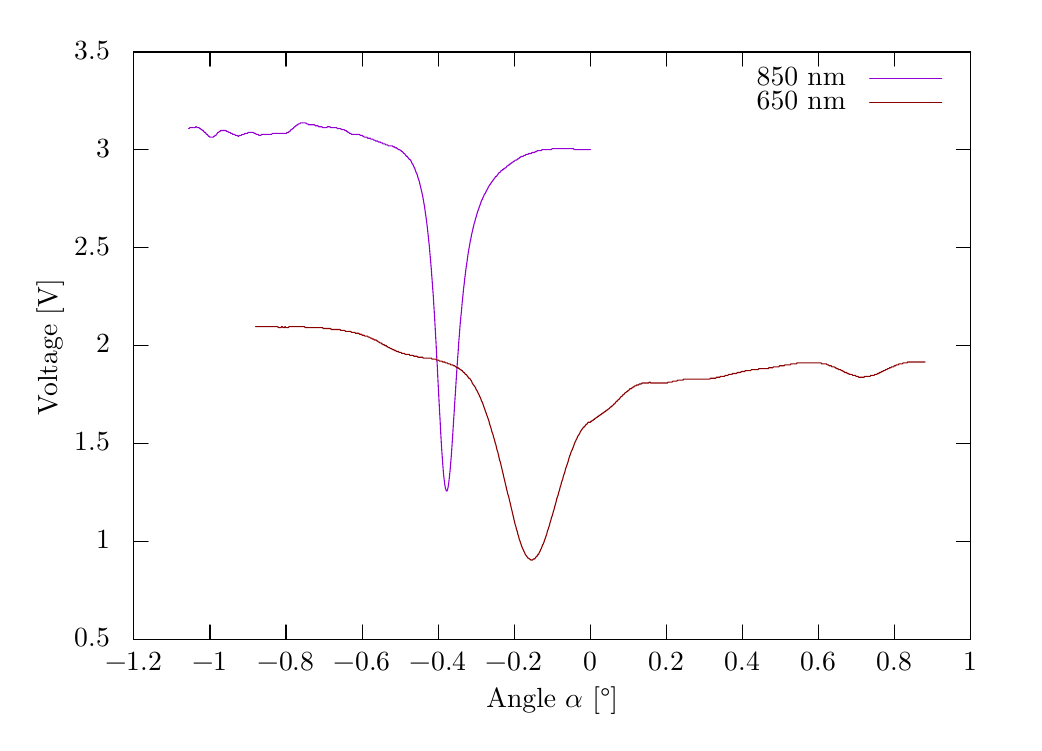
\begin{tikzpicture}[gnuplot]
%% generated with GNUPLOT 5.2p5a (Gentoo revision r0) (Lua 5.1; terminal rev. 99 , script rev. 107)
%% Mi 24 Apr 2019 10:58:10 CEST
\path (0.000,0.000) rectangle (12.500,8.750);
\gpcolor{color=gp lt color border}
\gpsetlinetype{gp lt border}
\gpsetdashtype{gp dt solid}
\gpsetlinewidth{1.00}
\draw[gp path] (1.320,0.985)--(1.500,0.985);
\draw[gp path] (11.947,0.985)--(11.767,0.985);
\node[gp node right] at (1.136,0.985) {$0.5$};
\draw[gp path] (1.320,2.228)--(1.500,2.228);
\draw[gp path] (11.947,2.228)--(11.767,2.228);
\node[gp node right] at (1.136,2.228) {$1$};
\draw[gp path] (1.320,3.470)--(1.500,3.470);
\draw[gp path] (11.947,3.470)--(11.767,3.470);
\node[gp node right] at (1.136,3.470) {$1.5$};
\draw[gp path] (1.320,4.713)--(1.500,4.713);
\draw[gp path] (11.947,4.713)--(11.767,4.713);
\node[gp node right] at (1.136,4.713) {$2$};
\draw[gp path] (1.320,5.956)--(1.500,5.956);
\draw[gp path] (11.947,5.956)--(11.767,5.956);
\node[gp node right] at (1.136,5.956) {$2.5$};
\draw[gp path] (1.320,7.198)--(1.500,7.198);
\draw[gp path] (11.947,7.198)--(11.767,7.198);
\node[gp node right] at (1.136,7.198) {$3$};
\draw[gp path] (1.320,8.441)--(1.500,8.441);
\draw[gp path] (11.947,8.441)--(11.767,8.441);
\node[gp node right] at (1.136,8.441) {$3.5$};
\draw[gp path] (1.320,0.985)--(1.320,1.165);
\draw[gp path] (1.320,8.441)--(1.320,8.261);
\node[gp node center] at (1.320,0.677) {$-1.2$};
\draw[gp path] (2.286,0.985)--(2.286,1.165);
\draw[gp path] (2.286,8.441)--(2.286,8.261);
\node[gp node center] at (2.286,0.677) {$-1$};
\draw[gp path] (3.252,0.985)--(3.252,1.165);
\draw[gp path] (3.252,8.441)--(3.252,8.261);
\node[gp node center] at (3.252,0.677) {$-0.8$};
\draw[gp path] (4.218,0.985)--(4.218,1.165);
\draw[gp path] (4.218,8.441)--(4.218,8.261);
\node[gp node center] at (4.218,0.677) {$-0.6$};
\draw[gp path] (5.184,0.985)--(5.184,1.165);
\draw[gp path] (5.184,8.441)--(5.184,8.261);
\node[gp node center] at (5.184,0.677) {$-0.4$};
\draw[gp path] (6.150,0.985)--(6.150,1.165);
\draw[gp path] (6.150,8.441)--(6.150,8.261);
\node[gp node center] at (6.150,0.677) {$-0.2$};
\draw[gp path] (7.117,0.985)--(7.117,1.165);
\draw[gp path] (7.117,8.441)--(7.117,8.261);
\node[gp node center] at (7.117,0.677) {$0$};
\draw[gp path] (8.083,0.985)--(8.083,1.165);
\draw[gp path] (8.083,8.441)--(8.083,8.261);
\node[gp node center] at (8.083,0.677) {$0.2$};
\draw[gp path] (9.049,0.985)--(9.049,1.165);
\draw[gp path] (9.049,8.441)--(9.049,8.261);
\node[gp node center] at (9.049,0.677) {$0.4$};
\draw[gp path] (10.015,0.985)--(10.015,1.165);
\draw[gp path] (10.015,8.441)--(10.015,8.261);
\node[gp node center] at (10.015,0.677) {$0.6$};
\draw[gp path] (10.981,0.985)--(10.981,1.165);
\draw[gp path] (10.981,8.441)--(10.981,8.261);
\node[gp node center] at (10.981,0.677) {$0.8$};
\draw[gp path] (11.947,0.985)--(11.947,1.165);
\draw[gp path] (11.947,8.441)--(11.947,8.261);
\node[gp node center] at (11.947,0.677) {$1$};
\draw[gp path] (1.320,8.441)--(1.320,0.985)--(11.947,0.985)--(11.947,8.441)--cycle;
\node[gp node center,rotate=-270] at (0.276,4.713) {Voltage [V]};
\node[gp node center] at (6.633,0.215) {Angle $\alpha$ [°]};
\node[gp node right] at (10.479,8.107) {850 nm};
\gpcolor{rgb color={0.580,0.000,0.827}}
\draw[gp path] (10.663,8.107)--(11.579,8.107);
\draw[gp path] (7.117,7.201)--(7.108,7.201)--(7.100,7.201)--(7.091,7.201)--(7.082,7.201)%
  --(7.074,7.201)--(7.065,7.201)--(7.057,7.201)--(7.048,7.201)--(7.040,7.201)--(7.031,7.201)%
  --(7.023,7.201)--(7.014,7.201)--(7.006,7.201)--(6.997,7.201)--(6.989,7.201)--(6.980,7.201)%
  --(6.972,7.201)--(6.963,7.201)--(6.955,7.201)--(6.946,7.201)--(6.938,7.201)--(6.929,7.201)%
  --(6.921,7.201)--(6.912,7.201)--(6.904,7.213)--(6.895,7.213)--(6.886,7.213)--(6.878,7.213)%
  --(6.869,7.213)--(6.861,7.213)--(6.852,7.213)--(6.844,7.213)--(6.835,7.213)--(6.827,7.213)%
  --(6.818,7.213)--(6.810,7.213)--(6.801,7.213)--(6.793,7.213)--(6.784,7.213)--(6.776,7.213)%
  --(6.767,7.213)--(6.759,7.213)--(6.750,7.213)--(6.742,7.213)--(6.733,7.213)--(6.725,7.213)%
  --(6.716,7.213)--(6.708,7.213)--(6.699,7.213)--(6.690,7.213)--(6.682,7.213)--(6.673,7.213)%
  --(6.665,7.213)--(6.656,7.213)--(6.648,7.213)--(6.639,7.213)--(6.631,7.213)--(6.622,7.201)%
  --(6.614,7.201)--(6.605,7.201)--(6.597,7.201)--(6.588,7.201)--(6.580,7.201)--(6.571,7.201)%
  --(6.563,7.201)--(6.554,7.201)--(6.546,7.201)--(6.537,7.201)--(6.529,7.201)--(6.520,7.201)%
  --(6.512,7.201)--(6.503,7.201)--(6.495,7.189)--(6.486,7.189)--(6.477,7.189)--(6.469,7.189)%
  --(6.460,7.189)--(6.452,7.189)--(6.443,7.189)--(6.435,7.176)--(6.426,7.176)--(6.418,7.176)%
  --(6.409,7.164)--(6.401,7.164)--(6.392,7.164)--(6.384,7.164)--(6.375,7.164)--(6.367,7.152)%
  --(6.358,7.152)--(6.350,7.152)--(6.341,7.152)--(6.333,7.152)--(6.324,7.140)--(6.316,7.140)%
  --(6.307,7.140)--(6.299,7.140)--(6.290,7.128)--(6.281,7.128)--(6.273,7.128)--(6.264,7.116)%
  --(6.256,7.116)--(6.247,7.116)--(6.239,7.116)--(6.230,7.104)--(6.222,7.104)--(6.213,7.091)%
  --(6.205,7.091)--(6.196,7.079)--(6.188,7.079)--(6.179,7.067)--(6.171,7.067)--(6.162,7.067)%
  --(6.154,7.055)--(6.145,7.055)--(6.137,7.043)--(6.128,7.043)--(6.120,7.031)--(6.111,7.031)%
  --(6.103,7.019)--(6.094,7.019)--(6.086,7.006)--(6.077,7.006)--(6.068,6.994)--(6.060,6.994)%
  --(6.051,6.982)--(6.043,6.970)--(6.034,6.970)--(6.026,6.958)--(6.017,6.958)--(6.009,6.946)%
  --(6.000,6.946)--(5.992,6.934)--(5.983,6.934)--(5.975,6.921)--(5.966,6.909)--(5.958,6.909)%
  --(5.949,6.897)--(5.941,6.885)--(5.932,6.873)--(5.924,6.861)--(5.915,6.861)--(5.907,6.848)%
  --(5.898,6.836)--(5.890,6.824)--(5.881,6.812)--(5.872,6.800)--(5.864,6.788)--(5.855,6.776)%
  --(5.847,6.763)--(5.838,6.751)--(5.830,6.739)--(5.821,6.727)--(5.813,6.703)--(5.804,6.691)%
  --(5.796,6.678)--(5.787,6.654)--(5.779,6.642)--(5.770,6.630)--(5.762,6.606)--(5.753,6.593)%
  --(5.745,6.569)--(5.736,6.557)--(5.728,6.533)--(5.719,6.508)--(5.711,6.484)--(5.702,6.460)%
  --(5.694,6.436)--(5.685,6.411)--(5.677,6.387)--(5.668,6.350)--(5.659,6.326)--(5.651,6.290)%
  --(5.642,6.265)--(5.634,6.229)--(5.625,6.193)--(5.617,6.156)--(5.608,6.120)--(5.600,6.071)%
  --(5.591,6.035)--(5.583,5.986)--(5.574,5.938)--(5.566,5.889)--(5.557,5.828)--(5.549,5.767)%
  --(5.540,5.707)--(5.532,5.646)--(5.523,5.573)--(5.515,5.500)--(5.506,5.427)--(5.498,5.342)%
  --(5.489,5.257)--(5.481,5.160)--(5.472,5.075)--(5.463,4.978)--(5.455,4.869)--(5.446,4.759)%
  --(5.438,4.638)--(5.429,4.516)--(5.421,4.395)--(5.412,4.261)--(5.404,4.127)--(5.395,3.994)%
  --(5.387,3.860)--(5.378,3.727)--(5.370,3.593)--(5.361,3.459)--(5.353,3.338)--(5.344,3.229)%
  --(5.336,3.131)--(5.327,3.046)--(5.319,2.974)--(5.310,2.913)--(5.302,2.876)--(5.293,2.864)%
  --(5.285,2.876)--(5.276,2.901)--(5.268,2.949)--(5.259,3.022)--(5.250,3.107)--(5.242,3.216)%
  --(5.233,3.338)--(5.225,3.459)--(5.216,3.617)--(5.208,3.775)--(5.199,3.933)--(5.191,4.091)%
  --(5.182,4.261)--(5.174,4.431)--(5.165,4.589)--(5.157,4.747)--(5.148,4.905)--(5.140,5.051)%
  --(5.131,5.196)--(5.123,5.330)--(5.114,5.452)--(5.106,5.561)--(5.097,5.682)--(5.089,5.779)%
  --(5.080,5.877)--(5.072,5.974)--(5.063,6.059)--(5.054,6.144)--(5.046,6.217)--(5.037,6.290)%
  --(5.029,6.350)--(5.020,6.411)--(5.012,6.472)--(5.003,6.521)--(4.995,6.569)--(4.986,6.618)%
  --(4.978,6.654)--(4.969,6.691)--(4.961,6.727)--(4.952,6.763)--(4.944,6.800)--(4.935,6.824)%
  --(4.927,6.848)--(4.918,6.885)--(4.910,6.897)--(4.901,6.921)--(4.893,6.946)--(4.884,6.970)%
  --(4.876,6.982)--(4.867,7.006)--(4.859,7.019)--(4.850,7.031)--(4.841,7.055)--(4.833,7.067)%
  --(4.824,7.079)--(4.816,7.079)--(4.807,7.091)--(4.799,7.104)--(4.790,7.116)--(4.782,7.116)%
  --(4.773,7.128)--(4.765,7.140)--(4.756,7.152)--(4.748,7.152)--(4.739,7.164)--(4.731,7.176)%
  --(4.722,7.176)--(4.714,7.189)--(4.705,7.189)--(4.697,7.201)--(4.688,7.201)--(4.680,7.201)%
  --(4.671,7.213)--(4.663,7.213)--(4.654,7.225)--(4.645,7.225)--(4.637,7.225)--(4.628,7.237)%
  --(4.620,7.237)--(4.611,7.237)--(4.603,7.249)--(4.594,7.249)--(4.586,7.249)--(4.577,7.249)%
  --(4.569,7.249)--(4.560,7.249)--(4.552,7.249)--(4.543,7.261)--(4.535,7.261)--(4.526,7.261)%
  --(4.518,7.261)--(4.509,7.274)--(4.501,7.274)--(4.492,7.274)--(4.484,7.274)--(4.475,7.286)%
  --(4.467,7.286)--(4.458,7.286)--(4.449,7.298)--(4.441,7.298)--(4.432,7.298)--(4.424,7.298)%
  --(4.415,7.310)--(4.407,7.310)--(4.398,7.310)--(4.390,7.310)--(4.381,7.322)--(4.373,7.322)%
  --(4.364,7.322)--(4.356,7.334)--(4.347,7.334)--(4.339,7.334)--(4.330,7.334)--(4.322,7.346)%
  --(4.313,7.346)--(4.305,7.346)--(4.296,7.346)--(4.288,7.346)--(4.279,7.359)--(4.271,7.359)%
  --(4.262,7.359)--(4.254,7.359)--(4.245,7.359)--(4.236,7.371)--(4.228,7.371)--(4.219,7.383)%
  --(4.211,7.383)--(4.202,7.383)--(4.194,7.383)--(4.185,7.395)--(4.177,7.395)--(4.168,7.395)%
  --(4.160,7.395)--(4.151,7.395)--(4.143,7.395)--(4.134,7.395)--(4.126,7.395)--(4.117,7.395)%
  --(4.109,7.395)--(4.100,7.395)--(4.092,7.395)--(4.083,7.395)--(4.075,7.407)--(4.066,7.407)%
  --(4.058,7.407)--(4.049,7.420)--(4.040,7.420)--(4.032,7.431)--(4.023,7.431)--(4.015,7.444)%
  --(4.006,7.444)--(3.998,7.444)--(3.989,7.456)--(3.981,7.456)--(3.972,7.456)--(3.964,7.456)%
  --(3.955,7.456)--(3.947,7.468)--(3.938,7.468)--(3.930,7.468)--(3.921,7.468)--(3.913,7.468)%
  --(3.904,7.468)--(3.896,7.480)--(3.887,7.480)--(3.879,7.480)--(3.870,7.480)--(3.862,7.480)%
  --(3.853,7.480)--(3.845,7.480)--(3.836,7.480)--(3.827,7.480)--(3.819,7.480)--(3.810,7.492)%
  --(3.802,7.492)--(3.793,7.492)--(3.785,7.492)--(3.776,7.492)--(3.768,7.480)--(3.759,7.480)%
  --(3.751,7.480)--(3.742,7.480)--(3.734,7.480)--(3.725,7.480)--(3.717,7.480)--(3.708,7.492)%
  --(3.700,7.492)--(3.691,7.492)--(3.683,7.492)--(3.674,7.492)--(3.666,7.492)--(3.657,7.505)%
  --(3.649,7.505)--(3.640,7.505)--(3.631,7.505)--(3.623,7.505)--(3.614,7.517)--(3.606,7.517)%
  --(3.597,7.517)--(3.589,7.517)--(3.580,7.517)--(3.572,7.517)--(3.563,7.517)--(3.555,7.517)%
  --(3.546,7.517)--(3.538,7.517)--(3.529,7.529)--(3.521,7.529)--(3.512,7.529)--(3.504,7.541)%
  --(3.495,7.541)--(3.487,7.541)--(3.478,7.541)--(3.470,7.541)--(3.461,7.541)--(3.453,7.541)%
  --(3.444,7.541)--(3.436,7.541)--(3.427,7.529)--(3.418,7.529)--(3.410,7.529)--(3.401,7.517)%
  --(3.393,7.517)--(3.384,7.505)--(3.376,7.505)--(3.367,7.492)--(3.359,7.492)--(3.350,7.480)%
  --(3.342,7.468)--(3.333,7.468)--(3.325,7.456)--(3.316,7.456)--(3.308,7.444)--(3.299,7.431)%
  --(3.291,7.431)--(3.282,7.420)--(3.274,7.420)--(3.265,7.420)--(3.257,7.407)--(3.248,7.407)%
  --(3.240,7.407)--(3.231,7.407)--(3.222,7.407)--(3.214,7.407)--(3.205,7.407)--(3.197,7.407)%
  --(3.188,7.407)--(3.180,7.407)--(3.171,7.407)--(3.163,7.407)--(3.154,7.407)--(3.146,7.407)%
  --(3.137,7.407)--(3.129,7.407)--(3.120,7.407)--(3.112,7.407)--(3.103,7.407)--(3.095,7.407)%
  --(3.086,7.407)--(3.078,7.407)--(3.069,7.395)--(3.061,7.395)--(3.052,7.395)--(3.044,7.395)%
  --(3.035,7.395)--(3.027,7.395)--(3.018,7.395)--(3.009,7.395)--(3.001,7.395)--(2.992,7.395)%
  --(2.984,7.395)--(2.975,7.395)--(2.967,7.395)--(2.958,7.395)--(2.950,7.395)--(2.941,7.395)%
  --(2.933,7.383)--(2.924,7.383)--(2.916,7.383)--(2.907,7.383)--(2.899,7.395)--(2.890,7.395)%
  --(2.882,7.395)--(2.873,7.395)--(2.865,7.407)--(2.856,7.407)--(2.848,7.407)--(2.839,7.420)%
  --(2.831,7.420)--(2.822,7.420)--(2.813,7.420)--(2.805,7.420)--(2.796,7.420)--(2.788,7.420)%
  --(2.779,7.420)--(2.771,7.420)--(2.762,7.407)--(2.754,7.407)--(2.745,7.407)--(2.737,7.407)%
  --(2.728,7.407)--(2.720,7.395)--(2.711,7.395)--(2.703,7.395)--(2.694,7.395)--(2.686,7.383)%
  --(2.677,7.383)--(2.669,7.383)--(2.660,7.383)--(2.652,7.371)--(2.643,7.371)--(2.635,7.383)%
  --(2.626,7.383)--(2.617,7.383)--(2.609,7.383)--(2.600,7.395)--(2.592,7.395)--(2.583,7.395)%
  --(2.575,7.395)--(2.566,7.407)--(2.558,7.407)--(2.549,7.407)--(2.541,7.420)--(2.532,7.420)%
  --(2.524,7.420)--(2.515,7.431)--(2.507,7.431)--(2.498,7.431)--(2.490,7.444)--(2.481,7.444)%
  --(2.473,7.444)--(2.464,7.444)--(2.456,7.444)--(2.447,7.444)--(2.439,7.444)--(2.430,7.444)%
  --(2.422,7.444)--(2.413,7.431)--(2.404,7.431)--(2.396,7.420)--(2.387,7.420)--(2.379,7.407)%
  --(2.370,7.395)--(2.362,7.383)--(2.353,7.383)--(2.345,7.371)--(2.336,7.371)--(2.328,7.359)%
  --(2.319,7.359)--(2.311,7.359)--(2.302,7.359)--(2.294,7.359)--(2.285,7.359)--(2.277,7.371)%
  --(2.268,7.371)--(2.260,7.383)--(2.251,7.395)--(2.243,7.395)--(2.234,7.407)--(2.226,7.420)%
  --(2.217,7.420)--(2.208,7.431)--(2.200,7.444)--(2.191,7.444)--(2.183,7.456)--(2.174,7.456)%
  --(2.166,7.468)--(2.157,7.468)--(2.149,7.480)--(2.140,7.480)--(2.132,7.480)--(2.123,7.480)%
  --(2.115,7.492)--(2.106,7.492)--(2.098,7.480)--(2.089,7.480)--(2.081,7.480)--(2.072,7.480)%
  --(2.064,7.480)--(2.055,7.480)--(2.047,7.480)--(2.038,7.480)--(2.030,7.480)--(2.021,7.468)%
  --(2.013,7.468);
\gpcolor{rgb color={0.545,0.000,0.000}}
\draw[gp path] (7.117,3.739)--(7.108,3.739)--(7.100,3.739)--(7.091,3.739)--(7.082,3.727)%
  --(7.074,3.714)--(7.065,3.714)--(7.057,3.702)--(7.048,3.690)--(7.040,3.678)--(7.031,3.678)%
  --(7.023,3.666)--(7.014,3.654)--(7.006,3.642)--(6.997,3.629)--(6.989,3.617)--(6.980,3.593)%
  --(6.972,3.581)--(6.963,3.569)--(6.955,3.557)--(6.946,3.532)--(6.938,3.520)--(6.929,3.496)%
  --(6.921,3.484)--(6.912,3.459)--(6.904,3.435)--(6.895,3.411)--(6.886,3.387)--(6.878,3.374)%
  --(6.869,3.350)--(6.861,3.326)--(6.852,3.302)--(6.844,3.277)--(6.835,3.241)--(6.827,3.216)%
  --(6.818,3.192)--(6.810,3.168)--(6.801,3.144)--(6.793,3.107)--(6.784,3.083)--(6.776,3.059)%
  --(6.767,3.022)--(6.759,2.998)--(6.750,2.974)--(6.742,2.937)--(6.733,2.913)--(6.725,2.876)%
  --(6.716,2.852)--(6.708,2.816)--(6.699,2.791)--(6.690,2.767)--(6.682,2.730)--(6.673,2.694)%
  --(6.665,2.670)--(6.656,2.633)--(6.648,2.609)--(6.639,2.573)--(6.631,2.548)--(6.622,2.524)%
  --(6.614,2.488)--(6.605,2.463)--(6.597,2.427)--(6.588,2.403)--(6.580,2.378)--(6.571,2.354)%
  --(6.563,2.318)--(6.554,2.293)--(6.546,2.269)--(6.537,2.245)--(6.529,2.220)--(6.520,2.196)%
  --(6.512,2.184)--(6.503,2.160)--(6.495,2.135)--(6.486,2.123)--(6.477,2.099)--(6.469,2.087)%
  --(6.460,2.062)--(6.452,2.062)--(6.443,2.038)--(6.435,2.038)--(6.426,2.026)--(6.418,2.014)%
  --(6.409,2.002)--(6.401,2.002)--(6.392,2.002)--(6.384,1.990)--(6.375,1.990)--(6.367,1.990)%
  --(6.358,1.990)--(6.350,2.002)--(6.341,2.002)--(6.333,2.014)--(6.324,2.014)--(6.316,2.026)%
  --(6.307,2.038)--(6.299,2.050)--(6.290,2.062)--(6.281,2.087)--(6.273,2.099)--(6.264,2.123)%
  --(6.256,2.135)--(6.247,2.160)--(6.239,2.184)--(6.230,2.208)--(6.222,2.233)--(6.213,2.257)%
  --(6.205,2.293)--(6.196,2.318)--(6.188,2.354)--(6.179,2.378)--(6.171,2.415)--(6.162,2.439)%
  --(6.154,2.475)--(6.145,2.512)--(6.137,2.548)--(6.128,2.585)--(6.120,2.621)--(6.111,2.658)%
  --(6.103,2.694)--(6.094,2.730)--(6.086,2.767)--(6.077,2.804)--(6.068,2.828)--(6.060,2.864)%
  --(6.051,2.901)--(6.043,2.937)--(6.034,2.974)--(6.026,3.010)--(6.017,3.046)--(6.009,3.083)%
  --(6.000,3.119)--(5.992,3.156)--(5.983,3.192)--(5.975,3.229)--(5.966,3.253)--(5.958,3.289)%
  --(5.949,3.326)--(5.941,3.362)--(5.932,3.387)--(5.924,3.423)--(5.915,3.459)--(5.907,3.484)%
  --(5.898,3.520)--(5.890,3.544)--(5.881,3.581)--(5.872,3.605)--(5.864,3.629)--(5.855,3.666)%
  --(5.847,3.690)--(5.838,3.714)--(5.830,3.751)--(5.821,3.775)--(5.813,3.800)--(5.804,3.824)%
  --(5.796,3.848)--(5.787,3.872)--(5.779,3.897)--(5.770,3.921)--(5.762,3.945)--(5.753,3.970)%
  --(5.745,3.994)--(5.736,4.006)--(5.728,4.030)--(5.719,4.055)--(5.711,4.067)--(5.702,4.091)%
  --(5.694,4.103)--(5.685,4.127)--(5.677,4.140)--(5.668,4.152)--(5.659,4.176)--(5.651,4.188)%
  --(5.642,4.200)--(5.634,4.212)--(5.625,4.225)--(5.617,4.237)--(5.608,4.261)--(5.600,4.273)%
  --(5.591,4.286)--(5.583,4.297)--(5.574,4.297)--(5.566,4.310)--(5.557,4.322)--(5.549,4.334)%
  --(5.540,4.346)--(5.532,4.346)--(5.523,4.358)--(5.515,4.371)--(5.506,4.371)--(5.498,4.383)%
  --(5.489,4.395)--(5.481,4.395)--(5.472,4.407)--(5.463,4.407)--(5.455,4.419)--(5.446,4.419)%
  --(5.438,4.431)--(5.429,4.431)--(5.421,4.431)--(5.412,4.443)--(5.404,4.443)--(5.395,4.456)%
  --(5.387,4.456)--(5.378,4.456)--(5.370,4.468)--(5.361,4.468)--(5.353,4.468)--(5.344,4.468)%
  --(5.336,4.480)--(5.327,4.480)--(5.319,4.480)--(5.310,4.480)--(5.302,4.492)--(5.293,4.492)%
  --(5.285,4.492)--(5.276,4.492)--(5.268,4.504)--(5.259,4.504)--(5.250,4.504)--(5.242,4.504)%
  --(5.233,4.516)--(5.225,4.516)--(5.216,4.516)--(5.208,4.516)--(5.199,4.516)--(5.191,4.528)%
  --(5.182,4.528)--(5.174,4.528)--(5.165,4.528)--(5.157,4.541)--(5.148,4.541)--(5.140,4.541)%
  --(5.131,4.541)--(5.123,4.541)--(5.114,4.541)--(5.106,4.541)--(5.097,4.553)--(5.089,4.553)%
  --(5.080,4.553)--(5.072,4.553)--(5.063,4.553)--(5.054,4.553)--(5.046,4.553)--(5.037,4.553)%
  --(5.029,4.553)--(5.020,4.553)--(5.012,4.553)--(5.003,4.553)--(4.995,4.553)--(4.986,4.565)%
  --(4.978,4.565)--(4.969,4.565)--(4.961,4.565)--(4.952,4.565)--(4.944,4.565)--(4.935,4.565)%
  --(4.927,4.565)--(4.918,4.577)--(4.910,4.577)--(4.901,4.577)--(4.893,4.577)--(4.884,4.577)%
  --(4.876,4.577)--(4.867,4.589)--(4.859,4.589)--(4.850,4.589)--(4.841,4.589)--(4.833,4.589)%
  --(4.824,4.589)--(4.816,4.601)--(4.807,4.601)--(4.799,4.601)--(4.790,4.601)--(4.782,4.601)%
  --(4.773,4.601)--(4.765,4.601)--(4.756,4.613)--(4.748,4.613)--(4.739,4.613)--(4.731,4.613)%
  --(4.722,4.613)--(4.714,4.626)--(4.705,4.626)--(4.697,4.626)--(4.688,4.626)--(4.680,4.638)%
  --(4.671,4.638)--(4.663,4.638)--(4.654,4.638)--(4.645,4.650)--(4.637,4.650)--(4.628,4.650)%
  --(4.620,4.662)--(4.611,4.662)--(4.603,4.662)--(4.594,4.674)--(4.586,4.674)--(4.577,4.674)%
  --(4.569,4.686)--(4.560,4.686)--(4.552,4.686)--(4.543,4.698)--(4.535,4.698)--(4.526,4.711)%
  --(4.518,4.711)--(4.509,4.711)--(4.501,4.723)--(4.492,4.723)--(4.484,4.723)--(4.475,4.735)%
  --(4.467,4.735)--(4.458,4.747)--(4.449,4.747)--(4.441,4.747)--(4.432,4.759)--(4.424,4.759)%
  --(4.415,4.771)--(4.407,4.771)--(4.398,4.783)--(4.390,4.783)--(4.381,4.783)--(4.373,4.783)%
  --(4.364,4.796)--(4.356,4.796)--(4.347,4.796)--(4.339,4.808)--(4.330,4.808)--(4.322,4.808)%
  --(4.313,4.820)--(4.305,4.820)--(4.296,4.820)--(4.288,4.832)--(4.279,4.832)--(4.271,4.832)%
  --(4.262,4.832)--(4.254,4.832)--(4.245,4.844)--(4.236,4.844)--(4.228,4.844)--(4.219,4.844)%
  --(4.211,4.856)--(4.202,4.856)--(4.194,4.856)--(4.185,4.856)--(4.177,4.869)--(4.168,4.869)%
  --(4.160,4.869)--(4.151,4.869)--(4.143,4.869)--(4.134,4.869)--(4.126,4.881)--(4.117,4.881)%
  --(4.109,4.881)--(4.100,4.881)--(4.092,4.881)--(4.083,4.881)--(4.075,4.893)--(4.066,4.893)%
  --(4.058,4.893)--(4.049,4.893)--(4.040,4.893)--(4.032,4.893)--(4.023,4.893)--(4.015,4.893)%
  --(4.006,4.893)--(3.998,4.905)--(3.989,4.905)--(3.981,4.905)--(3.972,4.905)--(3.964,4.905)%
  --(3.955,4.905)--(3.947,4.905)--(3.938,4.917)--(3.930,4.917)--(3.921,4.917)--(3.913,4.917)%
  --(3.904,4.917)--(3.896,4.917)--(3.887,4.917)--(3.879,4.917)--(3.870,4.917)--(3.862,4.917)%
  --(3.853,4.917)--(3.845,4.917)--(3.836,4.917)--(3.827,4.917)--(3.819,4.929)--(3.810,4.929)%
  --(3.802,4.929)--(3.793,4.929)--(3.785,4.929)--(3.776,4.929)--(3.768,4.929)--(3.759,4.929)%
  --(3.751,4.929)--(3.742,4.929)--(3.734,4.929)--(3.725,4.929)--(3.717,4.941)--(3.708,4.941)%
  --(3.700,4.941)--(3.691,4.941)--(3.683,4.941)--(3.674,4.941)--(3.666,4.941)--(3.657,4.941)%
  --(3.649,4.941)--(3.640,4.941)--(3.631,4.941)--(3.623,4.941)--(3.614,4.941)--(3.606,4.941)%
  --(3.597,4.941)--(3.589,4.941)--(3.580,4.941)--(3.572,4.941)--(3.563,4.941)--(3.555,4.941)%
  --(3.546,4.941)--(3.538,4.941)--(3.529,4.941)--(3.521,4.941)--(3.512,4.941)--(3.504,4.941)%
  --(3.495,4.941)--(3.487,4.954)--(3.478,4.954)--(3.470,4.954)--(3.461,4.954)--(3.453,4.954)%
  --(3.444,4.954)--(3.436,4.954)--(3.427,4.954)--(3.418,4.954)--(3.410,4.954)--(3.401,4.954)%
  --(3.393,4.954)--(3.384,4.954)--(3.376,4.954)--(3.367,4.954)--(3.359,4.954)--(3.350,4.954)%
  --(3.342,4.954)--(3.333,4.954)--(3.325,4.954)--(3.316,4.954)--(3.308,4.954)--(3.299,4.954)%
  --(3.291,4.954)--(3.282,4.941)--(3.274,4.941)--(3.265,4.941)--(3.257,4.941)--(3.248,4.941)%
  --(3.240,4.954)--(3.231,4.941)--(3.222,4.941)--(3.214,4.941)--(3.205,4.954)--(3.197,4.954)%
  --(3.188,4.941)--(3.180,4.941)--(3.171,4.941)--(3.163,4.941)--(3.154,4.941)--(3.146,4.954)%
  --(3.137,4.954)--(3.129,4.954)--(3.120,4.954)--(3.112,4.954)--(3.103,4.954)--(3.095,4.954)%
  --(3.086,4.954)--(3.078,4.954)--(3.069,4.954)--(3.061,4.954)--(3.052,4.954)--(3.044,4.954)%
  --(3.035,4.954)--(3.027,4.954)--(3.018,4.954)--(3.009,4.954)--(3.001,4.954)--(2.992,4.954)%
  --(2.984,4.954)--(2.975,4.954)--(2.967,4.954)--(2.958,4.954)--(2.950,4.954)--(2.941,4.954)%
  --(2.933,4.954)--(2.924,4.954)--(2.916,4.954)--(2.907,4.954)--(2.899,4.954)--(2.890,4.954)%
  --(2.882,4.954)--(2.873,4.954)--(2.865,4.954);
\gpcolor{color=gp lt color border}
\node[gp node right] at (10.479,7.799) {650 nm};
\gpcolor{rgb color={0.545,0.000,0.000}}
\draw[gp path] (10.663,7.799)--(11.579,7.799);
\draw[gp path] (7.117,3.739)--(7.125,3.751)--(7.134,3.751)--(7.142,3.763)--(7.151,3.763)%
  --(7.159,3.775)--(7.168,3.775)--(7.176,3.787)--(7.185,3.787)--(7.193,3.800)--(7.202,3.800)%
  --(7.210,3.812)--(7.219,3.812)--(7.227,3.824)--(7.236,3.824)--(7.244,3.836)--(7.253,3.836)%
  --(7.261,3.848)--(7.270,3.848)--(7.278,3.860)--(7.287,3.860)--(7.295,3.872)--(7.304,3.872)%
  --(7.313,3.885)--(7.321,3.885)--(7.330,3.897)--(7.338,3.897)--(7.347,3.909)--(7.355,3.909)%
  --(7.364,3.921)--(7.372,3.933)--(7.381,3.933)--(7.389,3.945)--(7.398,3.945)--(7.406,3.957)%
  --(7.415,3.970)--(7.423,3.970)--(7.432,3.982)--(7.440,3.994)--(7.449,4.006)--(7.457,4.006)%
  --(7.466,4.018)--(7.474,4.030)--(7.483,4.030)--(7.491,4.042)--(7.500,4.055)--(7.509,4.067)%
  --(7.517,4.067)--(7.526,4.079)--(7.534,4.091)--(7.543,4.091)--(7.551,4.103)--(7.560,4.115)%
  --(7.568,4.115)--(7.577,4.127)--(7.585,4.127)--(7.594,4.140)--(7.602,4.140)--(7.611,4.152)%
  --(7.619,4.164)--(7.628,4.164)--(7.636,4.164)--(7.645,4.176)--(7.653,4.176)--(7.662,4.188)%
  --(7.670,4.188)--(7.679,4.200)--(7.687,4.200)--(7.696,4.200)--(7.704,4.212)--(7.713,4.212)%
  --(7.722,4.212)--(7.730,4.212)--(7.739,4.225)--(7.747,4.225)--(7.756,4.225)--(7.764,4.225)%
  --(7.773,4.237)--(7.781,4.237)--(7.790,4.237)--(7.798,4.237)--(7.807,4.237)--(7.815,4.237)%
  --(7.824,4.237)--(7.832,4.237)--(7.841,4.237)--(7.849,4.237)--(7.858,4.237)--(7.866,4.249)%
  --(7.875,4.249)--(7.883,4.237)--(7.892,4.237)--(7.900,4.237)--(7.909,4.237)--(7.918,4.237)%
  --(7.926,4.237)--(7.935,4.237)--(7.943,4.237)--(7.952,4.237)--(7.960,4.237)--(7.969,4.237)%
  --(7.977,4.237)--(7.986,4.237)--(7.994,4.237)--(8.003,4.237)--(8.011,4.237)--(8.020,4.237)%
  --(8.028,4.237)--(8.037,4.237)--(8.045,4.237)--(8.054,4.237)--(8.062,4.237)--(8.071,4.237)%
  --(8.079,4.237)--(8.088,4.237)--(8.096,4.237)--(8.105,4.249)--(8.113,4.249)--(8.122,4.249)%
  --(8.131,4.249)--(8.139,4.249)--(8.148,4.249)--(8.156,4.249)--(8.165,4.261)--(8.173,4.261)%
  --(8.182,4.261)--(8.190,4.261)--(8.199,4.261)--(8.207,4.261)--(8.216,4.261)--(8.224,4.273)%
  --(8.233,4.273)--(8.241,4.273)--(8.250,4.273)--(8.258,4.273)--(8.267,4.273)--(8.275,4.273)%
  --(8.284,4.273)--(8.292,4.273)--(8.301,4.286)--(8.309,4.286)--(8.318,4.286)--(8.327,4.286)%
  --(8.335,4.286)--(8.344,4.286)--(8.352,4.286)--(8.361,4.286)--(8.369,4.286)--(8.378,4.286)%
  --(8.386,4.286)--(8.395,4.286)--(8.403,4.286)--(8.412,4.286)--(8.420,4.286)--(8.429,4.286)%
  --(8.437,4.286)--(8.446,4.286)--(8.454,4.286)--(8.463,4.286)--(8.471,4.286)--(8.480,4.286)%
  --(8.488,4.286)--(8.497,4.286)--(8.505,4.286)--(8.514,4.286)--(8.522,4.286)--(8.531,4.286)%
  --(8.540,4.286)--(8.548,4.286)--(8.557,4.286)--(8.565,4.286)--(8.574,4.286)--(8.582,4.286)%
  --(8.591,4.286)--(8.599,4.286)--(8.608,4.286)--(8.616,4.286)--(8.625,4.286)--(8.633,4.286)%
  --(8.642,4.297)--(8.650,4.297)--(8.659,4.297)--(8.667,4.297)--(8.676,4.297)--(8.684,4.297)%
  --(8.693,4.297)--(8.701,4.297)--(8.710,4.297)--(8.718,4.310)--(8.727,4.310)--(8.736,4.310)%
  --(8.744,4.310)--(8.753,4.310)--(8.761,4.310)--(8.770,4.322)--(8.778,4.322)--(8.787,4.322)%
  --(8.795,4.322)--(8.804,4.322)--(8.812,4.322)--(8.821,4.322)--(8.829,4.334)--(8.838,4.334)%
  --(8.846,4.334)--(8.855,4.334)--(8.863,4.334)--(8.872,4.346)--(8.880,4.346)--(8.889,4.346)%
  --(8.897,4.346)--(8.906,4.346)--(8.914,4.346)--(8.923,4.358)--(8.932,4.358)--(8.940,4.358)%
  --(8.949,4.358)--(8.957,4.358)--(8.966,4.358)--(8.974,4.358)--(8.983,4.371)--(8.991,4.371)%
  --(9.000,4.371)--(9.008,4.371)--(9.017,4.371)--(9.025,4.371)--(9.034,4.383)--(9.042,4.383)%
  --(9.051,4.383)--(9.059,4.383)--(9.068,4.383)--(9.076,4.383)--(9.085,4.395)--(9.093,4.395)%
  --(9.102,4.395)--(9.110,4.395)--(9.119,4.395)--(9.127,4.395)--(9.136,4.395)--(9.145,4.395)%
  --(9.153,4.395)--(9.162,4.407)--(9.170,4.407)--(9.179,4.407)--(9.187,4.407)--(9.196,4.407)%
  --(9.204,4.407)--(9.213,4.407)--(9.221,4.407)--(9.230,4.407)--(9.238,4.407)--(9.247,4.407)%
  --(9.255,4.419)--(9.264,4.419)--(9.272,4.419)--(9.281,4.419)--(9.289,4.419)--(9.298,4.419)%
  --(9.306,4.419)--(9.315,4.419)--(9.323,4.419)--(9.332,4.419)--(9.341,4.419)--(9.349,4.419)%
  --(9.358,4.419)--(9.366,4.419)--(9.375,4.419)--(9.383,4.431)--(9.392,4.431)--(9.400,4.431)%
  --(9.409,4.431)--(9.417,4.431)--(9.426,4.431)--(9.434,4.431)--(9.443,4.443)--(9.451,4.443)%
  --(9.460,4.443)--(9.468,4.443)--(9.477,4.443)--(9.485,4.443)--(9.494,4.443)--(9.502,4.443)%
  --(9.511,4.443)--(9.519,4.456)--(9.528,4.456)--(9.536,4.456)--(9.545,4.456)--(9.554,4.456)%
  --(9.562,4.456)--(9.571,4.456)--(9.579,4.456)--(9.588,4.468)--(9.596,4.468)--(9.605,4.468)%
  --(9.613,4.468)--(9.622,4.468)--(9.630,4.468)--(9.639,4.468)--(9.647,4.468)--(9.656,4.468)%
  --(9.664,4.480)--(9.673,4.480)--(9.681,4.480)--(9.690,4.480)--(9.698,4.480)--(9.707,4.480)%
  --(9.715,4.480)--(9.724,4.480)--(9.732,4.480)--(9.741,4.492)--(9.750,4.492)--(9.758,4.492)%
  --(9.767,4.492)--(9.775,4.492)--(9.784,4.492)--(9.792,4.492)--(9.801,4.492)--(9.809,4.492)%
  --(9.818,4.492)--(9.826,4.492)--(9.835,4.492)--(9.843,4.492)--(9.852,4.492)--(9.860,4.492)%
  --(9.869,4.492)--(9.877,4.492)--(9.886,4.492)--(9.894,4.492)--(9.903,4.492)--(9.911,4.492)%
  --(9.920,4.492)--(9.928,4.492)--(9.937,4.492)--(9.945,4.492)--(9.954,4.492)--(9.963,4.492)%
  --(9.971,4.492)--(9.980,4.492)--(9.988,4.492)--(9.997,4.492)--(10.005,4.492)--(10.014,4.492)%
  --(10.022,4.492)--(10.031,4.492)--(10.039,4.492)--(10.048,4.492)--(10.056,4.480)--(10.065,4.480)%
  --(10.073,4.480)--(10.082,4.480)--(10.090,4.480)--(10.099,4.480)--(10.107,4.480)--(10.116,4.480)%
  --(10.124,4.468)--(10.133,4.468)--(10.141,4.468)--(10.150,4.456)--(10.159,4.456)--(10.167,4.456)%
  --(10.176,4.456)--(10.184,4.443)--(10.193,4.443)--(10.201,4.443)--(10.210,4.443)--(10.218,4.443)%
  --(10.227,4.431)--(10.235,4.431)--(10.244,4.419)--(10.252,4.419)--(10.261,4.419)--(10.269,4.407)%
  --(10.278,4.407)--(10.286,4.407)--(10.295,4.407)--(10.303,4.395)--(10.312,4.395)--(10.320,4.395)%
  --(10.329,4.383)--(10.337,4.383)--(10.346,4.371)--(10.354,4.371)--(10.363,4.371)--(10.372,4.371)%
  --(10.380,4.358)--(10.389,4.358)--(10.397,4.358)--(10.406,4.346)--(10.414,4.346)--(10.423,4.346)%
  --(10.431,4.346)--(10.440,4.346)--(10.448,4.334)--(10.457,4.334)--(10.465,4.334)--(10.474,4.334)%
  --(10.482,4.334)--(10.491,4.322)--(10.499,4.322)--(10.508,4.322)--(10.516,4.322)--(10.525,4.310)%
  --(10.533,4.310)--(10.542,4.310)--(10.550,4.310)--(10.559,4.310)--(10.568,4.310)--(10.576,4.310)%
  --(10.585,4.310)--(10.593,4.310)--(10.602,4.322)--(10.610,4.322)--(10.619,4.322)--(10.627,4.322)%
  --(10.636,4.322)--(10.644,4.322)--(10.653,4.322)--(10.661,4.322)--(10.670,4.322)--(10.678,4.334)%
  --(10.687,4.334)--(10.695,4.334)--(10.704,4.334)--(10.712,4.334)--(10.721,4.334)--(10.729,4.346)%
  --(10.738,4.346)--(10.746,4.346)--(10.755,4.346)--(10.763,4.358)--(10.772,4.358)--(10.781,4.358)%
  --(10.789,4.371)--(10.798,4.371)--(10.806,4.371)--(10.815,4.383)--(10.823,4.383)--(10.832,4.383)%
  --(10.840,4.395)--(10.849,4.395)--(10.857,4.395)--(10.866,4.407)--(10.874,4.407)--(10.883,4.407)%
  --(10.891,4.419)--(10.900,4.419)--(10.908,4.419)--(10.917,4.431)--(10.925,4.431)--(10.934,4.431)%
  --(10.942,4.443)--(10.951,4.443)--(10.959,4.443)--(10.968,4.443)--(10.977,4.456)--(10.985,4.456)%
  --(10.994,4.456)--(11.002,4.468)--(11.011,4.468)--(11.019,4.468)--(11.028,4.468)--(11.036,4.480)%
  --(11.045,4.480)--(11.053,4.480)--(11.062,4.480)--(11.070,4.480)--(11.079,4.480)--(11.087,4.492)%
  --(11.096,4.492)--(11.104,4.492)--(11.113,4.492)--(11.121,4.492)--(11.130,4.492)--(11.138,4.492)%
  --(11.147,4.504)--(11.155,4.504)--(11.164,4.504)--(11.173,4.504)--(11.181,4.504)--(11.190,4.504)%
  --(11.198,4.504)--(11.207,4.504)--(11.215,4.504)--(11.224,4.504)--(11.232,4.504)--(11.241,4.504)%
  --(11.249,4.504)--(11.258,4.504)--(11.266,4.504)--(11.275,4.504)--(11.283,4.504)--(11.292,4.504)%
  --(11.300,4.504)--(11.309,4.504)--(11.317,4.504)--(11.326,4.504)--(11.334,4.504)--(11.343,4.504)%
  --(11.351,4.504)--(11.360,4.504)--(11.368,4.504);
\gpcolor{color=gp lt color border}
\draw[gp path] (1.320,8.441)--(1.320,0.985)--(11.947,0.985)--(11.947,8.441)--cycle;
%% coordinates of the plot area
\gpdefrectangularnode{gp plot 1}{\pgfpoint{1.320cm}{0.985cm}}{\pgfpoint{11.947cm}{8.441cm}}
\end{tikzpicture}
%% gnuplot variables

	\caption{The same silver coating of 45 nm at two different laser wavelengths of 650 nm and 850 nm}
\end{figure}
\begin{figure}
	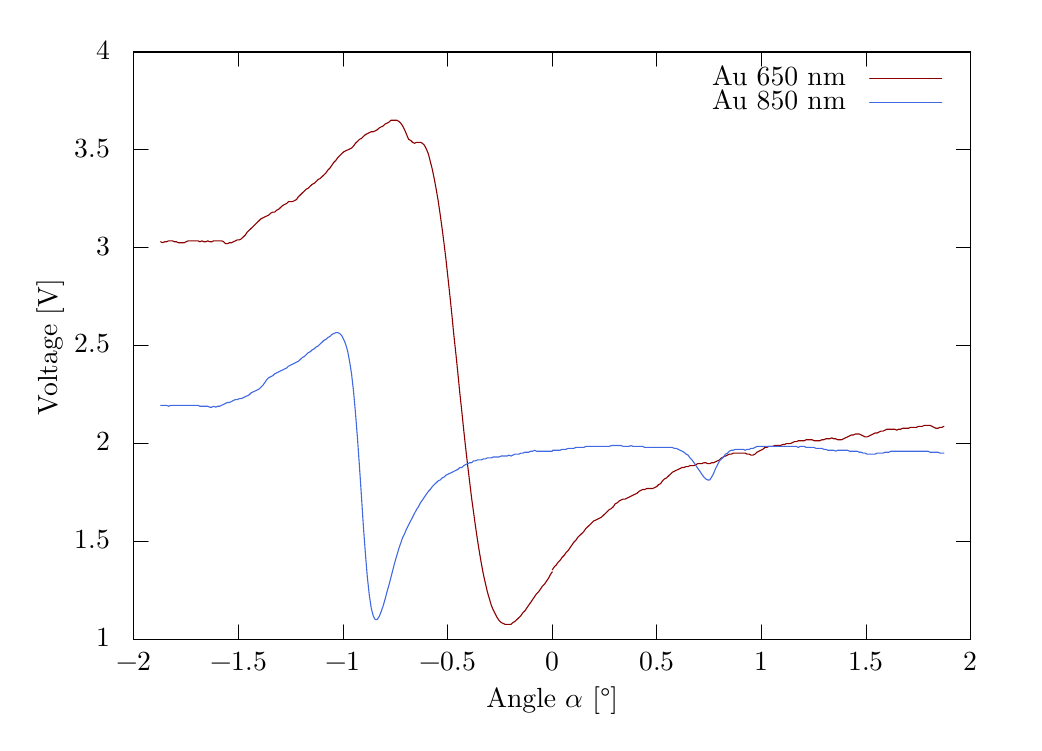
\begin{tikzpicture}[gnuplot]
%% generated with GNUPLOT 5.2p5a (Gentoo revision r0) (Lua 5.1; terminal rev. 99 , script rev. 107)
%% Mi 01 Mai 2019 12:56:06 CEST
\path (0.000,0.000) rectangle (12.500,8.750);
\gpcolor{color=gp lt color border}
\gpsetlinetype{gp lt border}
\gpsetdashtype{gp dt solid}
\gpsetlinewidth{1.00}
\draw[gp path] (1.320,0.985)--(1.500,0.985);
\draw[gp path] (11.947,0.985)--(11.767,0.985);
\node[gp node right] at (1.136,0.985) {$1$};
\draw[gp path] (1.320,2.228)--(1.500,2.228);
\draw[gp path] (11.947,2.228)--(11.767,2.228);
\node[gp node right] at (1.136,2.228) {$1.5$};
\draw[gp path] (1.320,3.470)--(1.500,3.470);
\draw[gp path] (11.947,3.470)--(11.767,3.470);
\node[gp node right] at (1.136,3.470) {$2$};
\draw[gp path] (1.320,4.713)--(1.500,4.713);
\draw[gp path] (11.947,4.713)--(11.767,4.713);
\node[gp node right] at (1.136,4.713) {$2.5$};
\draw[gp path] (1.320,5.956)--(1.500,5.956);
\draw[gp path] (11.947,5.956)--(11.767,5.956);
\node[gp node right] at (1.136,5.956) {$3$};
\draw[gp path] (1.320,7.198)--(1.500,7.198);
\draw[gp path] (11.947,7.198)--(11.767,7.198);
\node[gp node right] at (1.136,7.198) {$3.5$};
\draw[gp path] (1.320,8.441)--(1.500,8.441);
\draw[gp path] (11.947,8.441)--(11.767,8.441);
\node[gp node right] at (1.136,8.441) {$4$};
\draw[gp path] (1.320,0.985)--(1.320,1.165);
\draw[gp path] (1.320,8.441)--(1.320,8.261);
\node[gp node center] at (1.320,0.677) {$-2$};
\draw[gp path] (2.648,0.985)--(2.648,1.165);
\draw[gp path] (2.648,8.441)--(2.648,8.261);
\node[gp node center] at (2.648,0.677) {$-1.5$};
\draw[gp path] (3.977,0.985)--(3.977,1.165);
\draw[gp path] (3.977,8.441)--(3.977,8.261);
\node[gp node center] at (3.977,0.677) {$-1$};
\draw[gp path] (5.305,0.985)--(5.305,1.165);
\draw[gp path] (5.305,8.441)--(5.305,8.261);
\node[gp node center] at (5.305,0.677) {$-0.5$};
\draw[gp path] (6.634,0.985)--(6.634,1.165);
\draw[gp path] (6.634,8.441)--(6.634,8.261);
\node[gp node center] at (6.634,0.677) {$0$};
\draw[gp path] (7.962,0.985)--(7.962,1.165);
\draw[gp path] (7.962,8.441)--(7.962,8.261);
\node[gp node center] at (7.962,0.677) {$0.5$};
\draw[gp path] (9.290,0.985)--(9.290,1.165);
\draw[gp path] (9.290,8.441)--(9.290,8.261);
\node[gp node center] at (9.290,0.677) {$1$};
\draw[gp path] (10.619,0.985)--(10.619,1.165);
\draw[gp path] (10.619,8.441)--(10.619,8.261);
\node[gp node center] at (10.619,0.677) {$1.5$};
\draw[gp path] (11.947,0.985)--(11.947,1.165);
\draw[gp path] (11.947,8.441)--(11.947,8.261);
\node[gp node center] at (11.947,0.677) {$2$};
\draw[gp path] (1.320,8.441)--(1.320,0.985)--(11.947,0.985)--(11.947,8.441)--cycle;
\node[gp node center,rotate=-270] at (0.276,4.713) {Voltage [V]};
\node[gp node center] at (6.633,0.215) {Angle $\alpha$ [°]};
\node[gp node right] at (10.479,8.107) {Au 650 nm};
\gpcolor{rgb color={0.545,0.000,0.000}}
\draw[gp path] (10.663,8.107)--(11.579,8.107);
\draw[gp path] (6.634,1.865)--(6.658,1.901)--(6.683,1.925)--(6.708,1.962)--(6.733,1.986)%
  --(6.758,2.022)--(6.783,2.047)--(6.808,2.083)--(6.833,2.107)--(6.858,2.144)--(6.883,2.180)%
  --(6.908,2.217)--(6.933,2.241)--(6.958,2.277)--(6.983,2.302)--(7.008,2.326)--(7.033,2.350)%
  --(7.058,2.387)--(7.083,2.411)--(7.108,2.435)--(7.133,2.460)--(7.158,2.484)--(7.183,2.496)%
  --(7.208,2.508)--(7.233,2.520)--(7.258,2.533)--(7.283,2.557)--(7.308,2.581)--(7.333,2.605)%
  --(7.358,2.630)--(7.383,2.642)--(7.408,2.666)--(7.433,2.703)--(7.458,2.715)--(7.483,2.739)%
  --(7.508,2.751)--(7.533,2.763)--(7.558,2.763)--(7.583,2.775)--(7.608,2.788)--(7.633,2.800)%
  --(7.658,2.812)--(7.683,2.824)--(7.708,2.836)--(7.733,2.860)--(7.758,2.873)--(7.783,2.885)%
  --(7.808,2.885)--(7.833,2.897)--(7.858,2.897)--(7.883,2.897)--(7.908,2.897)--(7.933,2.909)%
  --(7.958,2.921)--(7.983,2.946)--(8.008,2.958)--(8.033,2.994)--(8.058,3.018)--(8.083,3.031)%
  --(8.108,3.055)--(8.133,3.079)--(8.158,3.103)--(8.183,3.116)--(8.208,3.128)--(8.233,3.140)%
  --(8.258,3.152)--(8.283,3.164)--(8.308,3.164)--(8.333,3.176)--(8.358,3.176)--(8.383,3.188)%
  --(8.408,3.188)--(8.433,3.188)--(8.458,3.201)--(8.483,3.213)--(8.508,3.213)--(8.533,3.213)%
  --(8.558,3.225)--(8.583,3.225)--(8.608,3.213)--(8.633,3.213)--(8.658,3.225)--(8.683,3.225)%
  --(8.708,3.237)--(8.733,3.249)--(8.758,3.261)--(8.783,3.286)--(8.808,3.298)--(8.833,3.310)%
  --(8.858,3.322)--(8.883,3.334)--(8.908,3.334)--(8.933,3.346)--(8.958,3.346)--(8.983,3.346)%
  --(9.008,3.346)--(9.033,3.346)--(9.058,3.346)--(9.083,3.346)--(9.108,3.334)--(9.133,3.334)%
  --(9.158,3.322)--(9.183,3.322)--(9.208,3.334)--(9.233,3.358)--(9.258,3.371)--(9.283,3.383)%
  --(9.308,3.395)--(9.333,3.419)--(9.358,3.419)--(9.383,3.432)--(9.408,3.432)--(9.433,3.432)%
  --(9.458,3.443)--(9.483,3.443)--(9.508,3.443)--(9.533,3.443)--(9.558,3.456)--(9.583,3.456)%
  --(9.608,3.468)--(9.633,3.468)--(9.658,3.468)--(9.683,3.480)--(9.708,3.492)--(9.733,3.492)%
  --(9.758,3.504)--(9.783,3.504)--(9.808,3.504)--(9.833,3.504)--(9.858,3.517)--(9.883,3.517)%
  --(9.908,3.517)--(9.933,3.517)--(9.958,3.504)--(9.983,3.504)--(10.008,3.504)--(10.033,3.504)%
  --(10.058,3.517)--(10.083,3.517)--(10.108,3.529)--(10.133,3.529)--(10.158,3.529)--(10.183,3.541)%
  --(10.208,3.529)--(10.233,3.529)--(10.258,3.517)--(10.283,3.517)--(10.308,3.517)--(10.333,3.529)%
  --(10.358,3.541)--(10.383,3.553)--(10.408,3.565)--(10.433,3.577)--(10.458,3.577)--(10.483,3.589)%
  --(10.508,3.589)--(10.533,3.589)--(10.558,3.577)--(10.583,3.565)--(10.608,3.553)--(10.633,3.553)%
  --(10.658,3.565)--(10.683,3.577)--(10.708,3.589)--(10.733,3.602)--(10.758,3.602)--(10.783,3.614)%
  --(10.808,3.626)--(10.833,3.626)--(10.858,3.638)--(10.883,3.650)--(10.908,3.650)--(10.933,3.650)%
  --(10.958,3.650)--(10.983,3.650)--(11.008,3.638)--(11.033,3.650)--(11.058,3.650)--(11.083,3.662)%
  --(11.108,3.662)--(11.133,3.662)--(11.158,3.662)--(11.183,3.674)--(11.208,3.674)--(11.233,3.674)%
  --(11.258,3.674)--(11.283,3.687)--(11.308,3.687)--(11.333,3.687)--(11.357,3.699)--(11.382,3.699)%
  --(11.407,3.699)--(11.432,3.699)--(11.457,3.687)--(11.482,3.674)--(11.507,3.662)--(11.532,3.662)%
  --(11.557,3.674)--(11.582,3.674)--(11.607,3.687);
\draw[gp path] (6.634,1.840)--(6.609,1.804)--(6.584,1.755)--(6.559,1.719)--(6.534,1.682)%
  --(6.509,1.658)--(6.484,1.621)--(6.459,1.585)--(6.434,1.561)--(6.409,1.524)--(6.384,1.488)%
  --(6.359,1.451)--(6.334,1.415)--(6.309,1.379)--(6.284,1.342)--(6.259,1.318)--(6.234,1.282)%
  --(6.209,1.257)--(6.184,1.233)--(6.159,1.208)--(6.134,1.196)--(6.109,1.172)--(6.084,1.172)%
  --(6.059,1.172)--(6.034,1.172)--(6.009,1.184)--(5.984,1.196)--(5.959,1.221)--(5.934,1.257)%
  --(5.909,1.306)--(5.884,1.354)--(5.859,1.415)--(5.834,1.500)--(5.809,1.585)--(5.784,1.694)%
  --(5.759,1.804)--(5.734,1.937)--(5.709,2.083)--(5.684,2.241)--(5.659,2.411)--(5.634,2.593)%
  --(5.609,2.775)--(5.584,2.982)--(5.559,3.188)--(5.534,3.407)--(5.509,3.638)--(5.484,3.881)%
  --(5.459,4.112)--(5.434,4.367)--(5.409,4.610)--(5.384,4.840)--(5.359,5.096)--(5.334,5.339)%
  --(5.309,5.569)--(5.284,5.800)--(5.259,6.007)--(5.234,6.201)--(5.209,6.383)--(5.184,6.553)%
  --(5.159,6.699)--(5.134,6.833)--(5.109,6.954)--(5.084,7.051)--(5.059,7.149)--(5.034,7.209)%
  --(5.009,7.258)--(4.984,7.282)--(4.959,7.294)--(4.934,7.294)--(4.909,7.294)--(4.884,7.282)%
  --(4.859,7.294)--(4.834,7.319)--(4.809,7.331)--(4.784,7.391)--(4.759,7.452)--(4.734,7.501)%
  --(4.709,7.537)--(4.684,7.561)--(4.659,7.574)--(4.634,7.574)--(4.609,7.574)--(4.584,7.574)%
  --(4.559,7.550)--(4.534,7.537)--(4.509,7.525)--(4.484,7.501)--(4.459,7.489)--(4.434,7.476)%
  --(4.409,7.452)--(4.384,7.440)--(4.359,7.428)--(4.334,7.428)--(4.309,7.416)--(4.284,7.404)%
  --(4.259,7.391)--(4.234,7.367)--(4.209,7.343)--(4.184,7.331)--(4.159,7.306)--(4.134,7.282)%
  --(4.109,7.246)--(4.084,7.221)--(4.059,7.209)--(4.034,7.197)--(4.009,7.185)--(3.984,7.173)%
  --(3.959,7.149)--(3.934,7.124)--(3.909,7.100)--(3.884,7.063)--(3.859,7.039)--(3.834,7.003)%
  --(3.809,6.966)--(3.784,6.942)--(3.759,6.906)--(3.734,6.881)--(3.709,6.857)--(3.684,6.833)%
  --(3.659,6.821)--(3.634,6.796)--(3.609,6.772)--(3.584,6.760)--(3.559,6.736)--(3.534,6.711)%
  --(3.509,6.699)--(3.484,6.675)--(3.459,6.651)--(3.434,6.626)--(3.409,6.602)--(3.384,6.566)%
  --(3.359,6.553)--(3.334,6.541)--(3.309,6.541)--(3.284,6.541)--(3.259,6.517)--(3.234,6.505)%
  --(3.209,6.492)--(3.184,6.468)--(3.159,6.444)--(3.134,6.432)--(3.109,6.408)--(3.084,6.408)%
  --(3.059,6.395)--(3.034,6.371)--(3.009,6.359)--(2.984,6.347)--(2.959,6.335)--(2.934,6.323)%
  --(2.909,6.298)--(2.884,6.274)--(2.859,6.250)--(2.834,6.225)--(2.809,6.201)--(2.784,6.177)%
  --(2.759,6.153)--(2.734,6.116)--(2.709,6.092)--(2.684,6.068)--(2.659,6.055)--(2.634,6.055)%
  --(2.609,6.043)--(2.584,6.031)--(2.559,6.019)--(2.534,6.019)--(2.509,6.007)--(2.484,6.007)%
  --(2.459,6.031)--(2.434,6.043)--(2.409,6.043)--(2.384,6.043)--(2.359,6.043)--(2.334,6.043)%
  --(2.309,6.031)--(2.284,6.031)--(2.259,6.043)--(2.234,6.031)--(2.209,6.031)--(2.184,6.043)%
  --(2.159,6.031)--(2.134,6.043)--(2.109,6.043)--(2.084,6.043)--(2.059,6.043)--(2.034,6.043)%
  --(2.009,6.043)--(1.984,6.031)--(1.959,6.019)--(1.934,6.019)--(1.910,6.019)--(1.885,6.019)%
  --(1.860,6.031)--(1.835,6.031)--(1.810,6.043)--(1.785,6.043)--(1.760,6.043)--(1.735,6.031)%
  --(1.710,6.031)--(1.685,6.019)--(1.660,6.031);
\gpcolor{color=gp lt color border}
\node[gp node right] at (10.479,7.799) {Au 850 nm};
\gpcolor{rgb color={0.255,0.412,0.882}}
\draw[gp path] (10.663,7.799)--(11.579,7.799);
\draw[gp path] (6.634,3.371)--(6.609,3.371)--(6.584,3.371)--(6.559,3.371)--(6.534,3.371)%
  --(6.509,3.371)--(6.484,3.371)--(6.459,3.371)--(6.434,3.371)--(6.409,3.383)--(6.384,3.371)%
  --(6.359,3.371)--(6.334,3.358)--(6.309,3.358)--(6.284,3.358)--(6.259,3.346)--(6.234,3.346)%
  --(6.209,3.334)--(6.184,3.334)--(6.159,3.334)--(6.134,3.322)--(6.109,3.310)--(6.084,3.322)%
  --(6.059,3.310)--(6.034,3.310)--(6.009,3.310)--(5.984,3.310)--(5.959,3.298)--(5.934,3.298)%
  --(5.909,3.298)--(5.884,3.298)--(5.859,3.286)--(5.834,3.286)--(5.809,3.286)--(5.784,3.273)%
  --(5.759,3.273)--(5.734,3.261)--(5.709,3.261)--(5.684,3.261)--(5.659,3.249)--(5.634,3.249)%
  --(5.609,3.225)--(5.584,3.225)--(5.559,3.213)--(5.534,3.201)--(5.509,3.188)--(5.484,3.164)%
  --(5.459,3.164)--(5.434,3.140)--(5.409,3.128)--(5.384,3.116)--(5.359,3.103)--(5.334,3.091)%
  --(5.309,3.079)--(5.284,3.067)--(5.259,3.043)--(5.234,3.031)--(5.209,3.006)--(5.184,2.994)%
  --(5.159,2.970)--(5.134,2.946)--(5.109,2.921)--(5.084,2.885)--(5.059,2.860)--(5.034,2.824)%
  --(5.009,2.788)--(4.984,2.751)--(4.959,2.715)--(4.934,2.666)--(4.909,2.630)--(4.884,2.581)%
  --(4.859,2.533)--(4.834,2.484)--(4.809,2.435)--(4.784,2.387)--(4.759,2.326)--(4.734,2.277)%
  --(4.709,2.205)--(4.684,2.132)--(4.659,2.047)--(4.634,1.962)--(4.609,1.865)--(4.584,1.767)%
  --(4.559,1.670)--(4.534,1.585)--(4.509,1.488)--(4.484,1.403)--(4.459,1.330)--(4.434,1.269)%
  --(4.409,1.233)--(4.384,1.233)--(4.359,1.282)--(4.334,1.379)--(4.309,1.549)--(4.284,1.779)%
  --(4.259,2.083)--(4.234,2.423)--(4.209,2.812)--(4.184,3.188)--(4.159,3.541)--(4.134,3.857)%
  --(4.109,4.136)--(4.084,4.355)--(4.059,4.513)--(4.034,4.646)--(4.009,4.731)--(3.984,4.792)%
  --(3.959,4.840)--(3.934,4.865)--(3.909,4.877)--(3.884,4.877)--(3.859,4.865)--(3.834,4.853)%
  --(3.809,4.828)--(3.784,4.816)--(3.759,4.792)--(3.734,4.780)--(3.709,4.755)--(3.684,4.731)%
  --(3.659,4.707)--(3.634,4.695)--(3.609,4.671)--(3.584,4.658)--(3.559,4.634)--(3.534,4.622)%
  --(3.509,4.598)--(3.484,4.573)--(3.459,4.561)--(3.434,4.537)--(3.409,4.513)--(3.384,4.501)%
  --(3.359,4.488)--(3.334,4.476)--(3.309,4.464)--(3.284,4.452)--(3.259,4.427)--(3.234,4.416)%
  --(3.209,4.403)--(3.184,4.391)--(3.159,4.379)--(3.134,4.367)--(3.109,4.355)--(3.084,4.330)%
  --(3.059,4.318)--(3.034,4.306)--(3.009,4.282)--(2.984,4.245)--(2.959,4.209)--(2.934,4.185)%
  --(2.909,4.160)--(2.884,4.148)--(2.859,4.136)--(2.834,4.124)--(2.809,4.112)--(2.784,4.087)%
  --(2.759,4.075)--(2.734,4.063)--(2.709,4.051)--(2.684,4.039)--(2.659,4.039)--(2.634,4.027)%
  --(2.609,4.027)--(2.584,4.015)--(2.559,4.002)--(2.534,3.990)--(2.509,3.990)--(2.484,3.978)%
  --(2.459,3.966)--(2.434,3.954)--(2.409,3.942)--(2.384,3.942)--(2.359,3.930)--(2.334,3.942)%
  --(2.309,3.930)--(2.284,3.930)--(2.259,3.942)--(2.234,3.942)--(2.209,3.942)--(2.184,3.942)%
  --(2.159,3.942)--(2.134,3.954)--(2.109,3.954)--(2.084,3.954)--(2.059,3.954)--(2.034,3.954)%
  --(2.009,3.954)--(1.984,3.954)--(1.959,3.954)--(1.934,3.954)--(1.910,3.954)--(1.885,3.954)%
  --(1.860,3.954)--(1.835,3.954)--(1.810,3.954)--(1.785,3.954)--(1.760,3.942)--(1.735,3.954)%
  --(1.710,3.954)--(1.685,3.954)--(1.660,3.954);
\draw[gp path] (6.634,3.383)--(6.658,3.383)--(6.683,3.383)--(6.708,3.383)--(6.733,3.383)%
  --(6.758,3.395)--(6.783,3.395)--(6.808,3.395)--(6.833,3.407)--(6.858,3.407)--(6.883,3.407)%
  --(6.908,3.407)--(6.933,3.419)--(6.958,3.419)--(6.983,3.419)--(7.008,3.419)--(7.033,3.419)%
  --(7.058,3.432)--(7.083,3.432)--(7.108,3.432)--(7.133,3.432)--(7.158,3.432)--(7.183,3.432)%
  --(7.208,3.432)--(7.233,3.432)--(7.258,3.432)--(7.283,3.432)--(7.308,3.432)--(7.333,3.432)%
  --(7.358,3.432)--(7.383,3.443)--(7.408,3.443)--(7.433,3.443)--(7.458,3.443)--(7.483,3.443)%
  --(7.508,3.443)--(7.533,3.432)--(7.558,3.432)--(7.583,3.432)--(7.608,3.432)--(7.633,3.443)%
  --(7.658,3.432)--(7.683,3.432)--(7.708,3.432)--(7.733,3.432)--(7.758,3.432)--(7.783,3.432)%
  --(7.808,3.419)--(7.833,3.419)--(7.858,3.419)--(7.883,3.419)--(7.908,3.419)--(7.933,3.419)%
  --(7.958,3.419)--(7.983,3.419)--(8.008,3.419)--(8.033,3.419)--(8.058,3.419)--(8.083,3.419)%
  --(8.108,3.419)--(8.133,3.419)--(8.158,3.419)--(8.183,3.407)--(8.208,3.407)--(8.233,3.395)%
  --(8.258,3.383)--(8.283,3.371)--(8.308,3.358)--(8.333,3.334)--(8.358,3.322)--(8.383,3.286)%
  --(8.408,3.261)--(8.433,3.225)--(8.458,3.188)--(8.483,3.152)--(8.508,3.116)--(8.533,3.079)%
  --(8.558,3.043)--(8.583,3.018)--(8.608,3.006)--(8.633,3.006)--(8.658,3.043)--(8.683,3.091)%
  --(8.708,3.152)--(8.733,3.201)--(8.758,3.249)--(8.783,3.273)--(8.808,3.298)--(8.833,3.334)%
  --(8.858,3.346)--(8.883,3.371)--(8.908,3.383)--(8.933,3.383)--(8.958,3.395)--(8.983,3.395)%
  --(9.008,3.395)--(9.033,3.395)--(9.058,3.395)--(9.083,3.383)--(9.108,3.395)--(9.133,3.395)%
  --(9.158,3.407)--(9.183,3.407)--(9.208,3.419)--(9.233,3.432)--(9.258,3.432)--(9.283,3.432)%
  --(9.308,3.432)--(9.333,3.432)--(9.358,3.432)--(9.383,3.432)--(9.408,3.432)--(9.433,3.432)%
  --(9.458,3.432)--(9.483,3.432)--(9.508,3.432)--(9.533,3.432)--(9.558,3.432)--(9.583,3.432)%
  --(9.608,3.432)--(9.633,3.432)--(9.658,3.432)--(9.683,3.432)--(9.708,3.432)--(9.733,3.432)%
  --(9.758,3.419)--(9.783,3.432)--(9.808,3.432)--(9.833,3.432)--(9.858,3.419)--(9.883,3.419)%
  --(9.908,3.419)--(9.933,3.419)--(9.958,3.419)--(9.983,3.407)--(10.008,3.407)--(10.033,3.407)%
  --(10.058,3.407)--(10.083,3.395)--(10.108,3.395)--(10.133,3.383)--(10.158,3.383)--(10.183,3.383)%
  --(10.208,3.383)--(10.233,3.371)--(10.258,3.383)--(10.283,3.383)--(10.308,3.383)--(10.333,3.383)%
  --(10.358,3.383)--(10.383,3.383)--(10.408,3.371)--(10.433,3.371)--(10.458,3.371)--(10.483,3.371)%
  --(10.508,3.371)--(10.533,3.358)--(10.558,3.358)--(10.583,3.346)--(10.608,3.346)--(10.633,3.334)%
  --(10.658,3.334)--(10.683,3.334)--(10.708,3.334)--(10.733,3.334)--(10.758,3.346)--(10.783,3.346)%
  --(10.808,3.346)--(10.833,3.346)--(10.858,3.358)--(10.883,3.358)--(10.908,3.358)--(10.933,3.371)%
  --(10.958,3.371)--(10.983,3.371)--(11.008,3.371)--(11.033,3.371)--(11.058,3.371)--(11.083,3.371)%
  --(11.108,3.371)--(11.133,3.371)--(11.158,3.371)--(11.183,3.371)--(11.208,3.371)--(11.233,3.371)%
  --(11.258,3.371)--(11.283,3.371)--(11.308,3.371)--(11.333,3.371)--(11.357,3.371)--(11.382,3.371)%
  --(11.407,3.371)--(11.432,3.358)--(11.457,3.358)--(11.482,3.358)--(11.507,3.358)--(11.532,3.358)%
  --(11.557,3.346)--(11.582,3.346)--(11.607,3.346);
\gpcolor{color=gp lt color border}
\draw[gp path] (1.320,8.441)--(1.320,0.985)--(11.947,0.985)--(11.947,8.441)--cycle;
%% coordinates of the plot area
\gpdefrectangularnode{gp plot 1}{\pgfpoint{1.320cm}{0.985cm}}{\pgfpoint{11.947cm}{8.441cm}}
\end{tikzpicture}
%% gnuplot variables

	\caption{The gold coating at the two wavelengths of 650 nm and 850 nm}
\end{figure}
\begin{figure}
	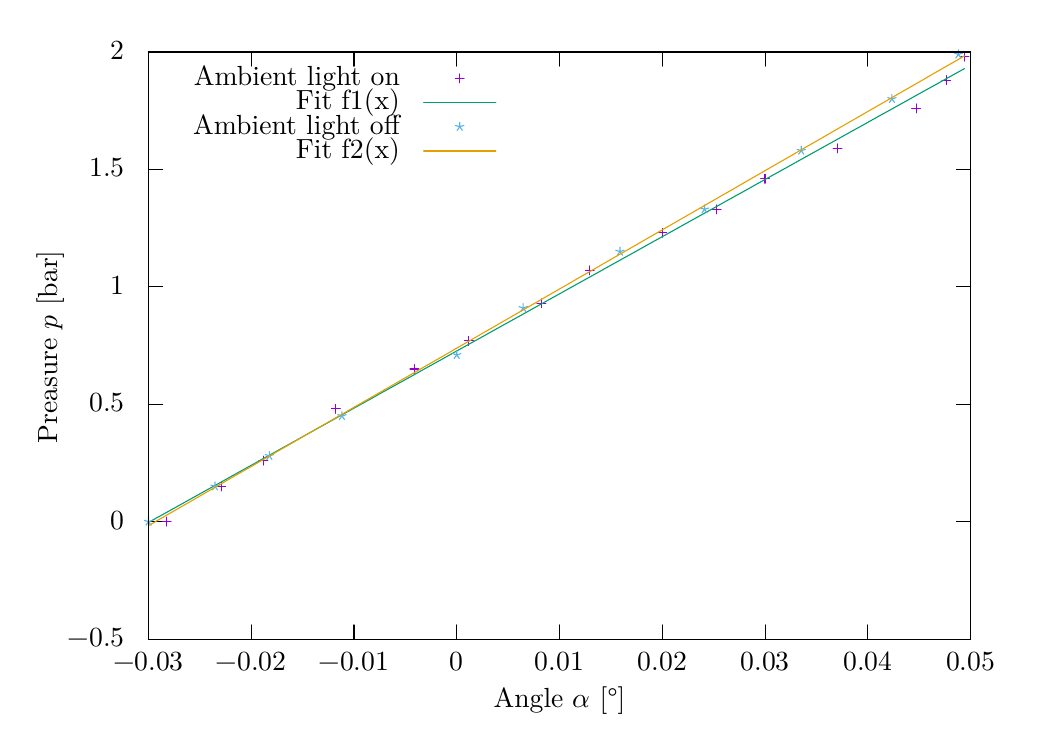
\begin{tikzpicture}[gnuplot]
%% generated with GNUPLOT 5.2p5a (Gentoo revision r0) (Lua 5.1; terminal rev. 99 , script rev. 107)
%% So 12 Mai 2019 19:50:21 CEST
\path (0.000,0.000) rectangle (12.500,8.750);
\gpcolor{color=gp lt color border}
\gpsetlinetype{gp lt border}
\gpsetdashtype{gp dt solid}
\gpsetlinewidth{1.00}
\draw[gp path] (1.504,0.985)--(1.684,0.985);
\draw[gp path] (11.947,0.985)--(11.767,0.985);
\node[gp node right] at (1.320,0.985) {$-0.5$};
\draw[gp path] (1.504,2.476)--(1.684,2.476);
\draw[gp path] (11.947,2.476)--(11.767,2.476);
\node[gp node right] at (1.320,2.476) {$0$};
\draw[gp path] (1.504,3.967)--(1.684,3.967);
\draw[gp path] (11.947,3.967)--(11.767,3.967);
\node[gp node right] at (1.320,3.967) {$0.5$};
\draw[gp path] (1.504,5.459)--(1.684,5.459);
\draw[gp path] (11.947,5.459)--(11.767,5.459);
\node[gp node right] at (1.320,5.459) {$1$};
\draw[gp path] (1.504,6.950)--(1.684,6.950);
\draw[gp path] (11.947,6.950)--(11.767,6.950);
\node[gp node right] at (1.320,6.950) {$1.5$};
\draw[gp path] (1.504,8.441)--(1.684,8.441);
\draw[gp path] (11.947,8.441)--(11.767,8.441);
\node[gp node right] at (1.320,8.441) {$2$};
\draw[gp path] (1.504,0.985)--(1.504,1.165);
\draw[gp path] (1.504,8.441)--(1.504,8.261);
\node[gp node center] at (1.504,0.677) {$-0.03$};
\draw[gp path] (2.809,0.985)--(2.809,1.165);
\draw[gp path] (2.809,8.441)--(2.809,8.261);
\node[gp node center] at (2.809,0.677) {$-0.02$};
\draw[gp path] (4.115,0.985)--(4.115,1.165);
\draw[gp path] (4.115,8.441)--(4.115,8.261);
\node[gp node center] at (4.115,0.677) {$-0.01$};
\draw[gp path] (5.420,0.985)--(5.420,1.165);
\draw[gp path] (5.420,8.441)--(5.420,8.261);
\node[gp node center] at (5.420,0.677) {$0$};
\draw[gp path] (6.726,0.985)--(6.726,1.165);
\draw[gp path] (6.726,8.441)--(6.726,8.261);
\node[gp node center] at (6.726,0.677) {$0.01$};
\draw[gp path] (8.031,0.985)--(8.031,1.165);
\draw[gp path] (8.031,8.441)--(8.031,8.261);
\node[gp node center] at (8.031,0.677) {$0.02$};
\draw[gp path] (9.336,0.985)--(9.336,1.165);
\draw[gp path] (9.336,8.441)--(9.336,8.261);
\node[gp node center] at (9.336,0.677) {$0.03$};
\draw[gp path] (10.642,0.985)--(10.642,1.165);
\draw[gp path] (10.642,8.441)--(10.642,8.261);
\node[gp node center] at (10.642,0.677) {$0.04$};
\draw[gp path] (11.947,0.985)--(11.947,1.165);
\draw[gp path] (11.947,8.441)--(11.947,8.261);
\node[gp node center] at (11.947,0.677) {$0.05$};
\draw[gp path] (1.504,8.441)--(1.504,0.985)--(11.947,0.985)--(11.947,8.441)--cycle;
\node[gp node center,rotate=-270] at (0.276,4.713) {Preasure $p$ [bar]};
\node[gp node center] at (6.725,0.215) {Angle $\alpha$ [°]};
\node[gp node right] at (4.816,8.107) {Ambient light on};
\gpcolor{rgb color={0.580,0.000,0.827}}
\gpsetpointsize{4.00}
\gppoint{gp mark 1}{(11.868,8.381)}
\gppoint{gp mark 1}{(11.637,8.083)}
\gppoint{gp mark 1}{(11.254,7.725)}
\gppoint{gp mark 1}{(10.256,7.218)}
\gppoint{gp mark 1}{(9.335,6.831)}
\gppoint{gp mark 1}{(8.721,6.443)}
\gppoint{gp mark 1}{(8.030,6.145)}
\gppoint{gp mark 1}{(7.109,5.667)}
\gppoint{gp mark 1}{(6.495,5.250)}
\gppoint{gp mark 1}{(5.574,4.773)}
\gppoint{gp mark 1}{(4.883,4.415)}
\gppoint{gp mark 1}{(3.885,3.908)}
\gppoint{gp mark 1}{(2.964,3.252)}
\gppoint{gp mark 1}{(2.427,2.924)}
\gppoint{gp mark 1}{(1.736,2.476)}
\gppoint{gp mark 1}{(5.458,8.107)}
\gpcolor{color=gp lt color border}
\node[gp node right] at (4.816,7.799) {Fit f1(x)};
\gpcolor{rgb color={0.000,0.620,0.451}}
\draw[gp path] (5.000,7.799)--(5.916,7.799);
\draw[gp path] (1.506,2.467)--(1.610,2.525)--(1.715,2.583)--(1.820,2.641)--(1.924,2.699)%
  --(2.029,2.758)--(2.134,2.816)--(2.238,2.874)--(2.343,2.932)--(2.448,2.990)--(2.552,3.049)%
  --(2.657,3.107)--(2.762,3.165)--(2.866,3.223)--(2.971,3.282)--(3.076,3.340)--(3.180,3.398)%
  --(3.285,3.456)--(3.390,3.514)--(3.494,3.573)--(3.599,3.631)--(3.704,3.689)--(3.808,3.747)%
  --(3.913,3.806)--(4.018,3.864)--(4.122,3.922)--(4.227,3.980)--(4.332,4.038)--(4.436,4.097)%
  --(4.541,4.155)--(4.646,4.213)--(4.750,4.271)--(4.855,4.329)--(4.960,4.388)--(5.064,4.446)%
  --(5.169,4.504)--(5.274,4.562)--(5.378,4.621)--(5.483,4.679)--(5.588,4.737)--(5.692,4.795)%
  --(5.797,4.853)--(5.902,4.912)--(6.006,4.970)--(6.111,5.028)--(6.216,5.086)--(6.320,5.144)%
  --(6.425,5.203)--(6.530,5.261)--(6.634,5.319)--(6.739,5.377)--(6.844,5.436)--(6.948,5.494)%
  --(7.053,5.552)--(7.158,5.610)--(7.262,5.668)--(7.367,5.727)--(7.472,5.785)--(7.576,5.843)%
  --(7.681,5.901)--(7.786,5.960)--(7.890,6.018)--(7.995,6.076)--(8.100,6.134)--(8.204,6.192)%
  --(8.309,6.251)--(8.414,6.309)--(8.518,6.367)--(8.623,6.425)--(8.728,6.483)--(8.832,6.542)%
  --(8.937,6.600)--(9.042,6.658)--(9.146,6.716)--(9.251,6.775)--(9.356,6.833)--(9.460,6.891)%
  --(9.565,6.949)--(9.670,7.007)--(9.774,7.066)--(9.879,7.124)--(9.984,7.182)--(10.088,7.240)%
  --(10.193,7.298)--(10.298,7.357)--(10.402,7.415)--(10.507,7.473)--(10.612,7.531)--(10.716,7.590)%
  --(10.821,7.648)--(10.926,7.706)--(11.030,7.764)--(11.135,7.822)--(11.240,7.881)--(11.344,7.939)%
  --(11.449,7.997)--(11.554,8.055)--(11.658,8.114)--(11.763,8.172)--(11.868,8.230);
\gpcolor{color=gp lt color border}
\node[gp node right] at (4.816,7.491) {Ambient light off};
\gpcolor{rgb color={0.337,0.706,0.914}}
\gppoint{gp mark 3}{(11.791,8.411)}
\gppoint{gp mark 3}{(10.947,7.845)}
\gppoint{gp mark 3}{(9.795,7.188)}
\gppoint{gp mark 3}{(8.567,6.443)}
\gppoint{gp mark 3}{(7.493,5.906)}
\gppoint{gp mark 3}{(6.264,5.190)}
\gppoint{gp mark 3}{(5.420,4.594)}
\gppoint{gp mark 3}{(3.962,3.818)}
\gppoint{gp mark 3}{(3.041,3.311)}
\gppoint{gp mark 3}{(2.350,2.924)}
\gppoint{gp mark 3}{(1.506,2.476)}
\gppoint{gp mark 3}{(5.458,7.491)}
\gpcolor{color=gp lt color border}
\node[gp node right] at (4.816,7.183) {Fit f2(x)};
\gpcolor{rgb color={0.902,0.624,0.000}}
\draw[gp path] (5.000,7.183)--(5.916,7.183);
\draw[gp path] (1.506,2.426)--(1.610,2.486)--(1.715,2.547)--(1.820,2.607)--(1.924,2.667)%
  --(2.029,2.727)--(2.134,2.788)--(2.238,2.848)--(2.343,2.908)--(2.448,2.968)--(2.552,3.029)%
  --(2.657,3.089)--(2.762,3.149)--(2.866,3.209)--(2.971,3.270)--(3.076,3.330)--(3.180,3.390)%
  --(3.285,3.450)--(3.390,3.511)--(3.494,3.571)--(3.599,3.631)--(3.704,3.692)--(3.808,3.752)%
  --(3.913,3.812)--(4.018,3.872)--(4.122,3.933)--(4.227,3.993)--(4.332,4.053)--(4.436,4.113)%
  --(4.541,4.174)--(4.646,4.234)--(4.750,4.294)--(4.855,4.354)--(4.960,4.415)--(5.064,4.475)%
  --(5.169,4.535)--(5.274,4.595)--(5.378,4.656)--(5.483,4.716)--(5.588,4.776)--(5.692,4.836)%
  --(5.797,4.897)--(5.902,4.957)--(6.006,5.017)--(6.111,5.077)--(6.216,5.138)--(6.320,5.198)%
  --(6.425,5.258)--(6.530,5.319)--(6.634,5.379)--(6.739,5.439)--(6.844,5.499)--(6.948,5.560)%
  --(7.053,5.620)--(7.158,5.680)--(7.262,5.740)--(7.367,5.801)--(7.472,5.861)--(7.576,5.921)%
  --(7.681,5.981)--(7.786,6.042)--(7.890,6.102)--(7.995,6.162)--(8.100,6.222)--(8.204,6.283)%
  --(8.309,6.343)--(8.414,6.403)--(8.518,6.463)--(8.623,6.524)--(8.728,6.584)--(8.832,6.644)%
  --(8.937,6.704)--(9.042,6.765)--(9.146,6.825)--(9.251,6.885)--(9.356,6.946)--(9.460,7.006)%
  --(9.565,7.066)--(9.670,7.126)--(9.774,7.187)--(9.879,7.247)--(9.984,7.307)--(10.088,7.367)%
  --(10.193,7.428)--(10.298,7.488)--(10.402,7.548)--(10.507,7.608)--(10.612,7.669)--(10.716,7.729)%
  --(10.821,7.789)--(10.926,7.849)--(11.030,7.910)--(11.135,7.970)--(11.240,8.030)--(11.344,8.090)%
  --(11.449,8.151)--(11.554,8.211)--(11.658,8.271)--(11.763,8.331)--(11.868,8.392);
\gpcolor{color=gp lt color border}
\draw[gp path] (1.504,8.441)--(1.504,0.985)--(11.947,0.985)--(11.947,8.441)--cycle;
%% coordinates of the plot area
\gpdefrectangularnode{gp plot 1}{\pgfpoint{1.504cm}{0.985cm}}{\pgfpoint{11.947cm}{8.441cm}}
\end{tikzpicture}
%% gnuplot variables

	\caption{Manual messurements of the pressure cell}
\end{figure}
\printbibliography
\end{document} 

